\documentclass{article}

\usepackage{graphicx} % Required for inserting images
\usepackage{kotex}
\usepackage{amssymb}
\usepackage{amsthm}
\usepackage[affil-it]{authblk}
\usepackage{fancyhdr}
\usepackage{braket}
\usepackage{dsfont}
\usepackage{bbold}
\usepackage{xcolor}
\usepackage{cite}
\usepackage{mathtools}
\usepackage{cancel}
\usepackage{esint}
\usepackage{subcaption}
\usepackage{enumitem}
\usepackage{geometry}
\usepackage{multicol}
\usepackage{color}
%\usepackage{times}
\usepackage{physics}
\usepackage{hyperref}

\newcommand{\vp}{\varphi}

\newtheorem{theorem}{Theorem}
\newtheorem{definition}[theorem]{Definition}
\newtheorem{example}[theorem]{Example}
\newtheorem{lemma}[theorem]{Lemma}
\newtheorem{axiom}[theorem]{Axiom}
\newtheorem{remark}[theorem]{Remark}
\newtheorem{problem}[theorem]{Problem}
\newtheorem{exercise}[theorem]{Exercise}

\counterwithin{equation}{section}
\counterwithin{theorem}{section}


\geometry{a4paper,left=2cm,right=2cm,top=2.4cm,bottom=2.4cm}

\linespread{1.3}

\title{\textsf{Mathematical Physics 2}}
\author[1]{Lectured by Stefano Scopel\thanks{email: scopel@sogang.ac.kr}}
\author[1]{Scribed by Eun Taek Kang\thanks{email: etkang03@gmail.com}}
\affil[1]{Department of Physics, Sogang University, Seoul 04107, Korea}

\date{Fall 2024, Sogang University}

\begin{document}

\pagestyle{fancy}
    %... then configure it.
    \fancyhf{}
    % Set the header and footer for Even
    % pages but omit the zone (L, C or R)
    \fancyhead[R]{\textsf{Prof. Stefano Scopel}}
    \fancyhead[L]{\textsc{Mathematical Physics 2}}
    \fancyfoot[C]{\thepage}
    \fancyfoot[L]{\textbf{Sogang University}}
    \fancyfoot[R]{\textit{Department of Physics}}

\maketitle

\begin{abstract}
    These are lecture notes that I typed up for Professor Stefano Scopel’s course and handout (PHY2006) on Mathematical Physics 2 in Fall 2024. The lecture was based on George B. Arfken's book, "Mathematical Methods for Physicists", 7th edition. I should note that these notes are not polished and hence might be riddled with errors. If you notice any typos or errors, please do contact me at etkang03@gmail.com
\end{abstract}

\newpage

\section{Handout 01}

\large
\begin{center}
    \textbf{Ordinary Differential Equations (ODE)}
\end{center}

\normalsize
\noindent
Many problems in Physics are formulated in terms of differential equations.
\begin{itemize}
    \item $x, y ,z, t, \cdots$ independent variables
    \item $f(x, y, \cdots), g(x, y, \cdots), \cdots$ dependent variables
\end{itemize}

\noindent
-- A differential equation with more than one independent variables is a partial differential equation (PDE).

\noindent
-- One indenepdent variable : ordinary differential equation (ODE).

\vspace{2mm}
\noindent
\textbf{Important feature}

\noindent
The derivative operator is \underline{linear}:
\begin{equation}
    \frac{d}{dx} [af(x) + bg(x)] = a \frac{df}{dx} + b \frac{dg}{dx}
\end{equation}
so it can be seen as a linear operator:
\begin{equation}
    \mathcal{L} \equiv \frac{d}{dx} \quad \Rightarrow \quad \mathcal{L} (af + bg) = a \mathcal{L} (f) + b \mathcal{L} (g)
\end{equation}
also higher derivatives are linear:
\begin{equation}
    \frac{d^n}{dx^n} [af(x) + bg(x)] = a \frac{d^n f}{dx^n} + b\frac{d^n g}{dx^n}
\end{equation}

\vspace{2mm}\noindent
\textbf{N.B.}

\noindent
If we define
\begin{equation}
    \mathcal{L} = p(x) \frac{d}{dx} + q(x)
\end{equation}
$\mathcal{L}$ is linear because it is still true that:
\begin{equation}
    \mathcal{L} (af + bg) = a \mathcal{L} (f) + b \mathcal{L} (g)
\end{equation}
even if $p(x)$ and $q(x)$ are not linear. \color{red}So, the general form of a linear differential operator is:
\color{black}
\begin{equation}
    \mathcal{L} = \sum_{n=0}^{N} p_n (x) \frac{d^n}{dx^n}
 \end{equation}
with $p_n(x)$ arbitrary functions.

\vspace{2mm}\noindent
An ODE is homogeneous if the dependent variables occurs to the same power in all terms. Otherwise in inhomogeneous -- A linear ODE has the form:
\begin{equation}
    \mathcal{L} \varphi(x) = F(x)
\end{equation}
with $\mathcal{L}$ a linear operator and $F(x)$ a function.

\vspace{2mm}\noindent
\textbf{N.B.} In $\mathcal{L} \varphi(x) = F(x)$, the term $F(x)$ does not contain $\varphi$ so the equation is inhomogeneous.

\noindent
Particular class of ODE's: both linear and homogeneous: $\mathcal{L} \varphi(x) = 0$

\noindent
In general the solution of an ODE is not unique. If there are many solution it is useful to identify those that are linear independent, i.e.
\begin{equation}
    \text{If} \ \ af_1 (x) + b f_2 (x) = 0 \ \text{for all }x \quad \Rightarrow \quad a, b = 0  
\end{equation}
with $a$, $b$ constants and $f_1$, $f_2$ two linear independent functions.

\newpage

\noindent
Homogeneous linear ODE's have the property that any linear combination of solutions is also a solution:
\begin{equation}
    \begin{cases}
        \mathcal{L} \varphi_1 (x) = 0 \\ \mathcal{L} \varphi_2 (x) = 0
    \end{cases} \quad \Rightarrow \quad \mathcal{L} (a \varphi_1 + b\varphi_2 ) = 0 \quad \text{with $a, b$ arbitrary constants}
\end{equation}
this is at the base of the \color{blue} Superposition principle \color{black} (the wave equation $\Delta \psi = \frac{1}{c^2} \frac{\partial^2 \psi}{\partial t^2}$ is linear!)

$\Rightarrow$ interference, refraction, etc in optics, quantum mechanics, etc ...

\noindent
Of course, many physical problems are nonlinear. (much more difficult, usually require numerical approaches)

\vspace{2mm}\noindent
Other definitions:
\begin{enumerate}
    \item order: highest derivative appearing in the ODE
    \item degree: power of the highest derivative after rationalization
\end{enumerate}

\noindent
\textbf{N.B.} only defined if the ODE is a polynomial in derivatives (transcendental functions of derivatives not allowed)

\begin{enumerate}
    \item $\left( \dfrac{d^2 y}{dx^2} \right)^3 + 2y \dfrac{d^4 y}{dx^4} = 0 \quad $ Order 4, Degree 1
    \item $y'' - \log y = (y'')^2 \quad $ Order 2, Degree 2.
    \item $\dfrac{d^2 s}{dt^2} + \left( \dfrac{ds}{dt} \right)^2 + \tan \left( \dfrac{ds}{dt} \right) + 1 = 0 \quad $ Order 2, Degree NOT DEFINED (by tan of derivative)
    \item $\sqrt{1 + \left( \dfrac{dy}{dx} \right)^2} = y \dfrac{d^3 y}{dx^3} \quad $ Not a polynomial but can be transformed into one by \color{red} Rationalization. \color{black}

    $ \Rightarrow 1 + \left( \dfrac{dy}{dx} \right)^2 = y^2 \left( \dfrac{d^3 y}{dx^3} \right)^2 \quad $ Order 3, Degree 2.
\end{enumerate}

\vspace{2mm}\noindent
\textbf{First order equations}

\noindent General form
\begin{equation}
    \frac{dy}{dx} = f(x, y) = -\frac{P(x, y)}{Q(x, y)}
\end{equation}
No systematic way to solve more general ones. Let's see some examples that can be solved.

\vspace{2mm}\noindent
\textbf{Seperable first order differential equations}

\noindent
Special form (NOT guaranteed!)
\begin{equation}
    \frac{dy}{dx} = - \frac{P(x)}{Q(y)}
\end{equation}
can rearrange it as
\begin{equation}
    P(x) dx + Q(y)dy = 0 \quad \Rightarrow \quad P(x)dx - -Q(y)dy
\end{equation}
can integrate both sides
\begin{equation}
    \int P(x)dx = - \int Q(y)dy
\end{equation}

\vspace{2mm}\noindent
\textbf{Example of parachute fall in air}
\begin{equation}
    m \dot{v} = mg - bv^2 \quad \text{(Newton's second law)} 
\end{equation}
as $t\rightarrow 0$ the right-hand side get to zero $\rightarrow$ No accelaration $\rightarrow$ Terminal velocity
\begin{equation}
    mg-bv^2 = 0 \quad \Rightarrow \quad v_t = \sqrt{\frac{mg}{b}}
\end{equation}

\newpage

\noindent
rewrite equation in terms of $v_0$:
\begin{equation}
    \frac{m}{b} \dot{v} = v_t ^ 2 - v^2 \ \ \Rightarrow \ \ \frac{m}{b} \frac{dv}{dt} = v_t ^ 2 - v^2 \ \ \Rightarrow \ \ \boxed{ \frac{dv}{v_t ^ 2 - v^2} = \frac{b}{m} dt } \ \ \text{(Separable)}
\end{equation}
so, integrate both sides
\begin{equation}
    \int_{v_0}^{v} \frac{dv}{v_t ^ 2 - v^2} = \frac{b}{m} \int_{v_0}^{v} dt \quad (v(t_0) = v_0 )
\end{equation}
setting $v_0 = 0$, $t_0 = 0$
\begin{equation}
    \int_{v_0}^{v} \frac{1}{2v_t} \left( \frac{1}{v + v_t} + \frac{1}{v - v_t} \right) dv = \frac{1}{2v_t} \ln \frac{v_t + v}{v_t - v}  = \frac{b}{m} t
\end{equation}
Done! but just need to solve for $v$.
\begin{equation}
    v = \frac{\exp{(2t/T)} - 1}{\exp{(2t/T)} + 1} v_0 = v_0 \tanh{(t/T)} \quad \left( T \equiv \sqrt{\frac{m}{gb}} \right)
\end{equation}

\vspace{2mm}\noindent
\textbf{Exact differential}

\noindent
The equation:
\begin{equation}
    P(x,y)dx + Q(x, y) dy = 0
\end{equation}
is \textbf{exact} if
\begin{equation}
    P(x, y)\,dx + Q(x, y)\,dy = d\varphi = \frac{\partial \varphi}{\partial x}\,dx + \frac{\partial \varphi}{\partial y}\,dy
\end{equation}
is the differential of a function $\varphi(x, y)$. $\varphi$ exists if
\begin{equation}
    P(x, y) = \frac{\partial \varphi}{\partial x}, \quad 
Q(x, y) = \frac{\partial \varphi}{\partial y} \ \ 
\Rightarrow \ \
\frac{\partial P}{\partial y} = \frac{\partial Q}{\partial x} 
= \frac{\partial^2 \varphi}{\partial x \partial y}
\end{equation}
So,
\begin{equation}
   \boxed{ \frac{\partial P(x, y)}{\partial y} = \frac{\partial Q(x, y)}{\partial x} }
\end{equation}

\noindent
\textbf{N.B.} If the equation is separable,
\begin{equation}
    P(x, y) = P(x) \Rightarrow \frac{\partial P}{\partial y} = 0 \ \  / \ \  Q(x, y) = Q(y) \Rightarrow \frac{\partial Q}{\partial x} = 0 \quad \Rightarrow \quad \frac{\partial P}{\partial y} = \frac{\partial Q}{\partial x} = 0 
\end{equation}
Separable equations are exact (the opposite is not necessarily true).

\vspace{2mm}\noindent
\textbf{Solution of exact equation}
\begin{equation}
    d\varphi = 0 \ \ \Rightarrow \ \  
\varphi = \int_{x_0}^{x} P(x, y)\,dx + \int_{y_0}^{y} Q(x, y)\,dy = \text{const.}
\end{equation}
\textbf{N.B.} the solutions are ``equipotential lines'' of the ``force'' $\vec{F} = (-P, -Q) \text{ with } \vec{F} = -\vec{\nabla} \varphi$.
\begin{figure}[h]
    \centering
    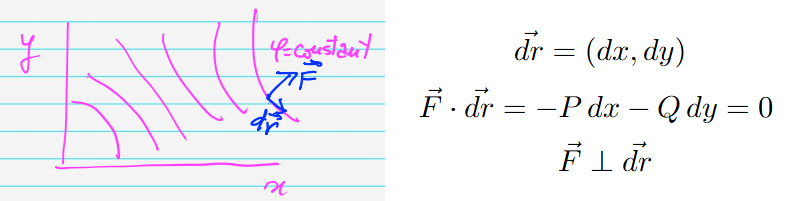
\includegraphics[width=0.75\linewidth]{fig1.png}
\end{figure}

\newpage

\noindent
\textbf{Example}
\begin{equation}
    y' + \left( 1 + \frac{y}{x} \right) = 0
\end{equation}
\begin{align*}
    &\Rightarrow \quad (x + y)\,dx + x\,dy = 0 \quad \textcolor{blue}{\text{(non separable)}}\\
    &\Rightarrow \quad P(x, y)\,dx + Q(x, y)\,dy = 0 \\
    &\Rightarrow \quad P(x, y) = x + y \ \ / \ \ Q(x,y) = x\\
    &\Rightarrow \quad \frac{\partial P}{\partial y} = 1, \quad 
\frac{\partial Q}{\partial x} = 1 \ \ \Rightarrow \ \ \boxed{\frac{\partial P}{\partial y} = \frac{\partial Q}{\partial x}} \quad \textcolor{red}{\text{(exact)}}
\end{align*}
then,
\begin{align*}
    & \quad \quad \varphi = Pdx + Qdy = 0\\
    &\Rightarrow \quad \varphi = \int_{x_0}^{x} (x + y)\,dy + \int_{y_0}^{y} x_0\,dy = \text{const.} \\
    &\Rightarrow \quad \frac{1}{2}(x^2 - x_0^2) + y(x - x_0) + x_0(y - y_0) = \text{const.}\\
    &\Rightarrow \quad \frac{x^2}{2} + xy + x_0 y - x_0 y = \text{const.}\\
    &\Rightarrow \quad \frac{x^2}{2} + xy = C
\end{align*}

\noindent
\textbf{N.B.} If the equation is not exact can find function $\alpha(x, y)$ so that: $\alpha P\,dx + \alpha Q\,dy = 0$ is exact (equivalent to solving it!)

\vspace{2mm}\noindent
\textbf{Equations homogeneous in $x$ and $y$}

\noindent
an ODE is homogeneous of order $n$ if in:
\begin{equation}
    P(x, y) dx + Q(x, y) dy = 0
\end{equation}
the combined powers of $x$ and $y$ add to $n$ in all the terms of $P$ and $Q$.

\noindent
\textbf{Example}
\begin{equation}
    (2x+ y)dx + xdy = 0 \quad (n=2)
\end{equation}
Make it separable with the substitution (change of variable).
\begin{align*}
    y = xv \ \  &\Rightarrow \quad dy = xdv + vdx\\
    &\Rightarrow \ \ \begin{cases}
        (2x+y) dx + xdy = 0 \\ y = xv \\ dy = xdv + vdx
    \end{cases}\\
    &\Rightarrow \quad (2x+xv)dx  + x(xdv + vdx) = 0\\
    &\Rightarrow \quad 2xdx + 2xvdx + x^2dv = 0
\end{align*}
Can simplify $x$ everywhere!
\begin{align*}
    & \quad \quad 2dx + 2vdx + xdv \ \ \Rightarrow \ \ 2(1+v)dx + xdv = 0 \\
    &\Rightarrow \ \  \frac{dx}{x} + \frac12 \frac{dv}{1+v} = 0 \ \ \Rightarrow \ \ \ln{x} + \frac12 \ln{(l+v)} = C \\
    &\Rightarrow \ \ \ln \left( x \sqrt{1 + v} \right) = C \ \ \Rightarrow \ \ x^2 (1 + v) = C \\
    &\Rightarrow \ \ x^2 \left(1 + \frac{y}{x} \right) = x^2 + xy = C
\end{align*}

\newpage

\noindent
Can generalize the definition of homogeneity by assigning different weight to $x$ and $y$ (same of $dx$ and $dy$). If assigning the weight 1 to $x$ and $m$ to $y$ makes the equation homogeneous (all terms same weight) one make the equation separable with the substitution:
\begin{equation}
    y = x^m v
\end{equation}
need to find $m$, if it exists.

\noindent
\textbf{Example}
\begin{equation}
    (x^2 - y)dx + xdy = 0 \quad \text{(not homogeneous)}
\end{equation}
assigning $x$ (weight 1), $y$ (weight $m$), then $x^2dx$ (weight 3), $ydx$ (weight $m+1$), $xdy$ (weight $m+1$). So, we solve following equation $3=m+1$ then $m=2$, $y = x^2v$.
\begin{equation}
    y = x^2 v \quad \Rightarrow \quad dy = 2xvdx + x^2 dv
\end{equation}
So, rewrite equation
\begin{align*}
    &\quad \quad (x^2 - y)dx + xdy = 0 \\ &\Rightarrow \ \ (x^2 - x^2 v)dx + x(2xvdx + x^2dv) = 0\\
    &\Rightarrow \ \  x^2dx - x^2 vdx + 2x^2 v dx + x^3 dv = 0\\
    &\Rightarrow \ \ dx-vdx +2vdx +xdv = 0\\ 
    &\Rightarrow \ \ (1+v)dx + xdv = 0 \quad (\text{Separable!)}\\
    &\Rightarrow \ \ \frac{dx}{x} = - \frac{dv}{1+v} \ \ \Rightarrow \ \ \ln{x} = - \ln{(1+v)} + C\\
    &\Rightarrow \ \  \ln{x}(1+v) = C \ \ \Rightarrow \ \ x(1+v) = C\\
    &\Rightarrow \ \  x\left( 1+\frac{y}{x^2} \right) = x+ \frac{y}{x} = C\\
    &\Rightarrow \ \ x^2 + y = cx \ \ \Rightarrow \ \ y = cx-x^2
\end{align*}

\vspace{2mm}\noindent
\textbf{Linear first order ODEs}
\begin{equation}
    \frac{dy}{dx} + P(x)y = Q(x)
\end{equation}
general solution exists, find function $\alpha(x)$ so that:
\begin{align*}
    &\quad \quad \alpha(x) \frac{dy}{dx} + \alpha(x) P(x) y = \frac{d}{dx} \left[ \alpha(x) y \right] \\
    &\Rightarrow \ \ \alpha(x) \frac{dy}{dx} + \alpha(x) P(x) y = y \frac{d\alpha}{dx} + \alpha(x) \frac{dy}{dx}\\
    &\Rightarrow \ \ \alpha(x) P(x) = \frac{d\alpha}{dx} \ \ \Rightarrow \ \ \frac{d\alpha}{\alpha} = P\,dx\\
    &\Rightarrow \ \ \ln \alpha = \int P\,dx + C\\
    &\Rightarrow \ \ \alpha(x) = C \exp\left( \int_{x_0}^{x} P(x)\,dx \right)
\end{align*}
Once $\alpha(x)$ is known directly solve:
\begin{align*}
    &\quad \quad \frac{d}{dx} \left[ \alpha(x)y \right] = \alpha(x)Q(x) \ \ \Rightarrow \ \ \alpha(x)y = \int \alpha(x)Q(x)\,dx \\
    &\Rightarrow \ \ y = \frac{1}{\alpha} \left[ \int \alpha(x) Q(x)\, dx + \text{const} \right] 
= \frac{C}{\alpha} + \frac{1}{\alpha} \int \alpha Q\, dx = y_1 + y_2
\end{align*}

\newpage

\noindent
\textbf{N.B.} If we set $Q(x)=0$ the equation becomes homogeneous with solution:
\begin{equation}
    \frac{dy}{dx} = P(x) y = 0 \ \ \Rightarrow \ \ \frac{dy}{y} + P(x)dx = 0 \ \ \Rightarrow \ \ \ln{y} + \int Pdx = \text{const}
\end{equation}
Using $\alpha = \exp \int Pdx$, then $\int Pdx = \ln \alpha$. Hence,
\begin{equation}
    \ln y + \ln \alpha = \text{const} \ \ \Rightarrow \ \ \alpha y = C \ \ \Rightarrow \ \ y = \frac{C}{\alpha} = y_1
\end{equation}
So, in
\begin{equation}
    y = \frac{C}{\alpha} + \frac{1}{\alpha} \int \alpha\, q\, dx
\end{equation}
$C/\alpha$ is solution of homogeneous equation where $Q(x) = 0$.

\noindent
On the other hand, $\frac{1}{\alpha} \int \alpha\, Q\, dx
$ is a particular solution of the equation (obtained setting the constant $c=0$)

\vspace{2mm}\noindent
\textbf{General Theorem}

\noindent
the solution of an inhomogeneous first order linear ode is the sum of a particular solution + an arbitrary multiple of a solution of the homogeneous equation obtained setting $Q=0$.

\noindent
In fact, if $y_1$ and $y_2$ are two solutions of the full equation:
\begin{equation}
    \frac{dy_1}{dx} + P(x)y_1 = Q(x) \ \ / \ \ \frac{dy_2}{dx} + P(x)y_2 = Q(x) \ \ \Rightarrow \ \ \frac{d}{dx}(y_1 - y_2) + P(x)(y_1 - y_2) = 0
\end{equation}
i.e. $cy = y_1 - y_2$ is a solution of the homogeneous equation $\Rightarrow \  y_1 = y_2 + cy$ when $y_2$ is particular solution of full ODE, $cy$ is solution of homogeneous ODE times arbitrary constant

\vspace{2mm}\noindent
\textbf{N.B. 2} A first order linear homogeneous ode has only one linearly independent solution. (linearly independent means: if $\alpha y_1 + \beta y_2 = 0 \Rightarrow \alpha = \beta = 0$.) Let’s assume two linearly independent solutions exist. then:
\begin{align*}
    &\quad \quad y_1' = -P y_1 \ \ / \ \ y_2' = -P y_2 \ \ \Rightarrow \ \  \frac{y_1'}{y_1} = -P = \frac{y_2'}{y_2} \\
    &\Rightarrow \ \ln y_1 = \ln y_2 + C  \ \ \Rightarrow y_1 = C y_2
\end{align*}
So, $y_1$ is proportional to $y_2$, $y_1$ and $y_2$ are not linearly independent.

\vspace{2mm}\noindent
\textbf{RL circuit}

\begin{figure}[h]
    \centering
    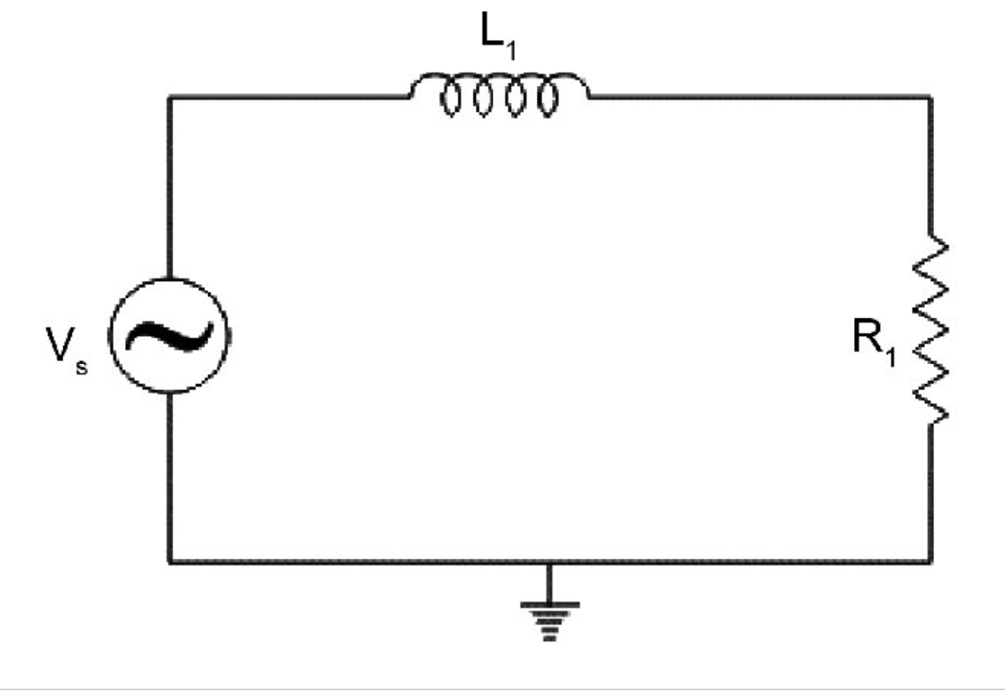
\includegraphics[width=0.3\linewidth]{fig2.png}
\end{figure}
\begin{equation}
    L \frac{dI(t)}{dt} + R I(t) = V(t)
\end{equation}
Solve homogeneous equation:
\begin{align*}
    & \quad \quad L\frac{dI}{dt} + RI = V(t) \quad \color{red}{(\text{separable!)}}\\
    &\Rightarrow \ \ \frac{dI}{I} = \frac{dt}{\tau}, \quad \tau \equiv \frac{L}{R} \Rightarrow I = C \exp\left( \frac{t}{\tau} \right)
\end{align*}
Look for one particular solution of the full equation (any is fine):

\newpage
\begin{equation}
    I= \frac{V_0}{R} \quad \text{(when the current is constant $V=V_0$  and the impedance resistivity is zero)}
\end{equation}
Full solution: sum of particular solution + homogeneous solution times arbitrary constant
\begin{equation}
    I = \frac{V_0}{R} + Ce^{t/\tau}
\end{equation}
fix constant $C$ with boundary conditions. For instance, if $I=0$ for $t=0$:
\begin{equation}
    \frac{V_0}{R} + C = 0 \ \  \Rightarrow \ \  C = -\frac{V_0}{R} \ \ \Rightarrow \ \  I = \frac{V_0}{R} ( 1 - e^{t/\tau} )
\end{equation}
\begin{figure}[h]
    \centering
    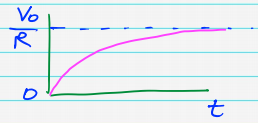
\includegraphics[width=0.3\linewidth]{fig3.png}
\end{figure}

\section{Handout 02}

\vspace{2mm}\noindent
\textbf{Homogeneous ODEs with constant coefficients}
\begin{equation}
    \frac{d^n y}{dx^n} + a_{n-1} \frac{d^{n-1} y}{dx^{n-1}} + \cdots + a_1 \frac{dy}{dx} + a_0 y = F(x)
\end{equation}
the homogeneous equation (with $F=0$) has solutions of the type:
\begin{equation}
    y=e^{mx}
\end{equation}
substituting, $m$ is solution of the algebraic equation:
\begin{equation}
    m^n + a_{n-1} m^{n-1} + \cdots + a_1 m + a_0 = 0
\end{equation}
which has $n$ solutions in the complex domain $m_1, m_2, \cdots , m_n$. Then the general solution is their linear combination:
\begin{equation}
    y = C_1 e^{m_1 x} + C_2 e^{m_2 x} + \cdots + C_n e^{m_n x}
\end{equation}

\noindent
\textbf{N.B.} if the algebraic equation has multiple solutions one does not get $n$ values for $m$. The missing solutions are of the type:
\begin{equation}
    e^{mx}, \quad x e^{mx}, \quad x^2 e^{mx}, \quad \ldots, \quad x^k e^{mx}
\end{equation}
if $m$ is a solution of multiplicity $k$. In this way one gets $n$ linearly independent solutions. 

\vspace{2mm}\noindent
\textbf{Second-order linear ODEs}
\begin{equation}
    y'' + P(x)y' + Q(x)y = 0 \quad (\text{homogeneous})
\end{equation}
\begin{itemize}
    \item A singular point $x_0$ is \textbf{regular} if either $P(x)$ or $Q(x)$ diverges there, but $(x - x_0) P(x)$ and $(x - x_0)^2 Q(x)$ remain finite.
    \item A singular point $x_0$ is \textbf{irregular} if $P(x)$ diverges faster than $1/(x - x_0)$ so that $(x - x_0) P(x)$ goes to infinity as $x \to x_0$, or if $Q(x)$ diverges faster than $1/(x - x_0)^2$ so that $(x - x_0)^2 Q(x)$ goes to infinity as $x \to x_0$.
\end{itemize}
\newpage

\noindent
Expand solution close to a regular point:
\begin{equation}
    y(x) = \sum_{j=0}^{\infty} a_j (x - x_0)^{s + j}, \quad a_0 \ne 0
\end{equation}
\textbf{N.B. } $a_0$ and $a_1$ are arbitrary, and must be fixed with boundary conditions. By substitution one gets a recursive relation that allows to obtain $a_2$, $a_3$, $\cdots$ as a function of $a_0$ and $a_1$.

\noindent
Find $s$. Substitute expansion and take $x \rightarrow x_0$
\begin{align*}
    y = \sum_k a_k (x - x_0)^{k + s} \ \ / \ \  
y' = \sum_k (k + s) a_k (x - x_0)^{k + s - 1} \ \ / \ \ 
y'' = \sum_k (k + s)(k + s - 1) a_k (x - x_0)^{k + s - 2} \\
\Rightarrow \sum_k (k + s)(k + s - 1) a_k (x - x_0)^{k + s} 
+ P(x) \sum_k (k + s) a_k (x - x_0)^{k + s} 
+ Q(x) \sum_k a_k (x - x_0)^{k + s} = 0
\end{align*}
set $k=0$:
\begin{equation}
    a_0 \left[ s(s-1)(x - x_0)^{s-2} + P(x)\, s(x - x_0)^{s-1} + Q(x)(x - x_0)^s \right] = 0
\end{equation}
take limit $x \rightarrow x_0$:
\begin{equation}
    a_0 (x - x_0)^{s - 2} \left[s(s - 1) + \lim_{x \to x_0} P(x)(x - x_0)s + \lim_{x \to x_0} Q(x)(x - x_0)^2 \right] = 0
\end{equation}
\textbf{N.B.} If the limits:
\begin{equation}
    \left\{
\begin{aligned}
&\lim_{x \to x_0} P(x)(x - x_0) = p_0 \\
&\lim_{x \to x_0} Q(x)(x - x_0)^2 = q_0
\end{aligned}
\right.
\end{equation}
exist then $x_0$ is regular, as $s$ is a solution of the Fuchs or indicial equation:
\begin{equation}
    s(s - 1) + p_0 s + q_0 = 0
\end{equation}
the equation is quadratic, so it has two solutions $s_1$ and $s_2$. However, in general, only if $s1-s2\neq$ integer the two power expansions for $s_1$ and $s_2$ correspond to two linearly independent solutions of the ODE.

\noindent
One we know $s$ the coefficients $a_k$ are found explicitly (use $x_0=0$ for simplicity):
\begin{equation}
    y = \sum_{k=0}^{\infty} a_k x^{k+s}  \ \ / \ \ y' = \sum_{k=0}^{\infty} a_k (k+s) x^{k+s-1} \ \ / \ \ y'' = \sum_{k=0}^{\infty} a_k (k+s)(k+s-1) x^{k+s-2}
\end{equation}
substitute and rename $k \rightarrow k+1$ in $y'$ and $k \rightarrow k+2$ in $y''$:
\begin{align*}
    &\quad \quad \sum_k a_{k+2} (k+s+2)(k+s+1)\, x^{k+s} + P(x) \sum_k a_{k+1} (k+s+1)\, x^{k+s} + Q(x) \sum_k a_k\, x^{k+s} = 0\\
    &\Rightarrow \ \ \sum_k \left[ a_{k+2}(k+s+2)(k+s+1) + P\, a_{k+1}(k+s+1) + Q\, a_k \right] x^{k+s} = 0
\end{align*}
Recursive relation:
\begin{equation}
    a_{k+2}(k+s+2)(k+s+1) + P\, a_{k+1}(k+s+1) + Q\, a_k = 0
\end{equation}
knowing $a_0$ and $a_1$ can calculate $a_2$, then knowing $a_1$ and $a_2$ can get $a_3$, etc...

\vspace{2mm}\noindent
\textbf{N.B.} For two values of $s = s_1,\, s_1 - n$ one solution is:
\begin{equation}
    a_{k+2} (k + s_1 + 2)(k + s_1 + 1) + P\, a_{k+1} (k + s_1 + 1) + Q\, a_k = 0
\end{equation}
For $k=0$:
\begin{equation}
    a_2 (s_1 + 2)(s_1 + 1) + P\, a_1 (s_1 + 1) + Q\, a_0 = 0
\end{equation}

\newpage
\noindent
while the other is:
\begin{equation}
    a_{k+2} (k + s_1 - n + 2)(k + s_1 - n + 1) 
+ P\, a_{k+1} (k + s_1 - n + 1) 
+ Q\, a_k = 0
\end{equation}
for $k=n$,
\begin{equation}
    a_{k+2} (k + s_1 - n + 2)(k + s_1 - n + 1) + P\, a_{k+1} (k + s_1 - n + 1) + Q\, a_k = 0
\end{equation}
\begin{equation}
    a_{n+2} (s_1 + 2)(s_1 + 1) + P\, a_{n+1} (s_1 + 1) + Q\, a_n = 0
\end{equation}

\vspace{3mm}\noindent
\textbf{Fuchs' Theorem}

\noindent We can only obtain one power-series solution provided that we are expanding about a point which is 
an ordinary point, or at worst a regular singular point. 

\vspace{3mm}\noindent
In particular the indicial equation allows to find at least one solution. To find a second linearly independent solution one has to be careful. Let’s see step by step.

\noindent
Linearly independent solutions are such that if:
\begin{equation}
    \sum_{\lambda} k_{\lambda} \varphi_{\lambda}(x) = 0
\end{equation}
then $k_\lambda=0$. For a set of n solutions one can generate the following $n$ equations:
\begin{equation}
    \sum_{\lambda} k_{\lambda} \varphi_{\lambda}'(x) = 0 \ , \quad 
\sum_{\lambda} k_{\lambda} \varphi_{\lambda}''(x) = 0
\end{equation}
then can be seen as n linear equations in the variables $k_1$, $k_2$, $\cdots$, $k_n$. Such system has only one solution (the trivial one, $k_\lambda=0$, corresponding to the case of linear independence) only if its determinant is different from zero (for any $x$, i.e. the zero is the zero function):
\begin{equation}
    W \equiv \left|
\begin{array}{cccc}
\varphi_1 & \varphi_2 & \cdots & \varphi_n \\
\varphi_1' & \varphi_2' & \cdots & \varphi_n' \\
\vdots & \vdots & \ddots & \vdots \\
\varphi_1^{(n-1)} & \varphi_2^{(n-1)} & \cdots & \varphi_n^{(n-1)}
\end{array}
\right| \neq 0 \quad \color{red}{\text{(Wronskian)}} \color{black}
\end{equation}

\begin{theorem}
    A second-order homogeneous ODE has two linearly independent solutions.
\end{theorem}

\noindent
Can be proven by showing that if we assume a third solution their Wronskian is necessarily zero.

\noindent
Take three solutions: $y_1$, $y_2$, $y_3$.

\noindent
Wronskian of any pair: 
\begin{equation}
    W_{jk} = y_j y_k' - y_k y_j'
\end{equation}
take derivatives:
\begin{equation}
    W_{jk}' = y_j' y_k' + y_j y_k'' - y_k' y_j' - y_k y_j'' =  y_j y_k'' - y_k y_j''
\end{equation}
divide ODE by y and move Q to the right:
\begin{equation}
    \frac{y''}{y} + P \frac{y'}{y} = -Q 
\Rightarrow 
\frac{y_j''}{y_j} + P(x) \frac{y_j'}{y_j} = \frac{y_k''}{y_k} + P(x) \frac{y_k'}{y_k} = -Q(x)
\end{equation}
then:
\begin{equation}
    y_k \left( y_j'' - P y_j' \right) = y_j \left( y_k'' + P y_k' \right)
\end{equation}
\newpage
\noindent
By expression of Wronskian:
\begin{equation}
    W_{kj}' + P(x) W_{kj} = 0 \quad \Rightarrow \quad W_{kj}' = -P(x) W_{kj}
\end{equation}
calculate now the Wronskian of the three solutions:
\begin{equation}
W = 
\begin{vmatrix}
y_1 & y_2 & y_3 \\
y_1' & y_2' & y_3' \\
y_1'' & y_2'' & y_3''
\end{vmatrix}
= -y_1' W_{23}' + y_2' W_{13}' - y_3' W_{12}'
\end{equation}
Using:
\begin{equation}
    W_{23}' = -P W_{23}, \quad W_{13}' = -P W_{13}, \quad W_{12}' = -P W_{12}.
\end{equation}
\begin{equation}
    W' = P(x) \left( y_1' W_{23} + y_2' W_{13} + y_3' W_{12} \right)
= -P(x)
\begin{vmatrix}
y_1 & y_2 & y_3 \\
y_1' & y_2' & y_3' \\
y_1' & y_2' & y_3'
\end{vmatrix}
= 0
\end{equation}
So the Wronskian of three solutions necessarily vanishes $\rightarrow$ there are only two. \color{red}can be generalized to $n$-order homogenous ODEs. \color{black}

\vspace{2mm}\noindent
\textbf{Finding a second solution of a second-order ODE}

\noindent
Suppose you already know one solution $y_1$ (for instance, obtained as a power series or by guessing) You want to find a second solution $y_2$ such that the Wronskian $W = y_1 y_2' - y_1' y_2 \neq 0$.

\noindent
Use the already known relation:
\begin{equation}
    W' = -P(x) W
\end{equation}
(which implies that $W$ is constant when $P=0$)

\noindent
This is a separable first-order differential equation for $W$, with solution:
\begin{equation}
    \int_{W(a)}^{W(x)} \frac{dW}{W} = -\int_{a}^{x} P(x)\,dx 
\quad \Rightarrow \quad 
W(x) = W(a) \, e^{- \int_{a}^{x} P(x)\,dx}
\end{equation}
Combine with the identity
\begin{equation}
    W(x) = y_1 y_2' - y_1' y_2 
= y_1^2 \left[ \frac{y_2'}{y_1} - y_2 \cdot \frac{y_1'}{y_1 ^2} \right] 
= y_1^2 \left[ \frac{y_2'}{y_1} + y_2 \cdot \left(\frac{1}{y_1} \right)' \right] 
= y_1^2 \frac{d}{dx} \left( \frac{y_2}{y_1} \right)
\end{equation}
So that
\begin{equation}
y_1^2 \frac{d}{dx} \left( \frac{y_2}{y_1} \right) = W(a) \exp\left( -\int_a^x P(x') \, dx' \right)
\end{equation}
divide $y_1 ^2$,
\begin{equation}
    \frac{d}{dx} \left( \frac{y_2}{y_1} \right) = \frac{W(a)}{y_1 ^2} \exp\left( -\int_a^x P(x') \, dx' \right)
\end{equation}
then, 
\begin{equation}
    y_2(x) = y_1(x) \, W(a) \int_b^x \frac{1}{y_1^2(x')} \exp\left( -\int_a^{x'} P(x'') \, dx'' \right) dx'
\end{equation}
integrating from $x' = b$ to $x' = x$, can omit the lower bounds (that contribute a constant times $y_1$) and write:
\begin{equation}
y_2(x) = y_1(x) \int^x \frac{e^{ -\int^{x'} P(x'')\,dx'' }}{ \left[ y_1(x') \right]^2 } \, dx'
\end{equation}
\textbf{N.B.} In the case P=0 this simplifies to:
\begin{equation}
    y_2(x) = y_1(x) \int^x \frac{dx'}{[y_1(x')]^2}
\end{equation}
\newpage
\noindent
\textbf{Example:}
\begin{equation}
    \frac{d^2 y}{dx^2} + y = 0
\end{equation}
suppose we know one solution $y_1 = \sin{x}$. Then the second solution is ($P=0$):
\begin{equation}
    y_2(x) = \sin x \int^x \frac{dx'}{\sin^2(x')} 
= \sin x \left( -\int^x - \left[ \frac{\cos x'}{\sin x'} \right] dx' \right)
= -\sin x \cdot \frac{\cos x}{\sin x} = -\cos x
\end{equation}
\textbf{N.B.}
\begin{equation}
    W = \sin x \cdot \cos x' - \sin x' \cdot \cos x 
= \cos^2 x + \sin^2 x = 1 \quad \text{(constant)} \quad (P = 0)
\end{equation}
Now we are ready to look for a second solution of a second-order differential equation in series form around $x=x_0$. Let’s set for simplicity $x_0=0$.

\noindent
Write $P(x)$ and $Q(x)$ as:
\begin{equation}
    P(x) = \sum_{i=-1}^{\infty} p_i x^i \qquad 
Q(x) = \sum_{i=-2}^{\infty} q_i x^i
\end{equation}
\noindent
$i=-1$, $i=-2$ are allow for Fuchsian singularity. and:
\begin{equation}
    y = \sum_{k=0}^{\infty} a_k x^{s+k}
\end{equation}
We know that $s$ is solution of the indicial equation $s(s+1) + p_{-1} s + q_{-2} = 0$. Suppose that the two roots are $s_1 = a$ and $s_2 = a - n$ If $n$ is not an integer the two functions $y_1 \sim x^a$ and $y_2 \sim x^{a-n}$ have non vanishing Wronskian in $x = x_0$ and so also for $x \neq x_0 $ using
\begin{equation}
    W(x) = W(x_0) \, e^{-\int_{x_0}^{x} P(x')\,dx'}
\end{equation}
So if the difference of the two solutions of the indicial equation is not an integer they correspond to the two linearly independent solutions. However if $s_1 - s_2 = n \in \mathbb{Z}$ one can see that the second solution requires an additional logarithmic term. Let’s see why. The indicial equation with solutions $s_1$ and $s_2$ can be written as:
\begin{align*}
    & \quad \quad (s - s_1)(s- s_2) = 0 \ \ \Rightarrow \ \ (s - \alpha)(s-\alpha + n) = 0 \\
    & \Rightarrow \ \ s^2 + (n-2\alpha)s+\alpha(\alpha-n)=0 \ \ \Rightarrow \ \ p_{-1} - 1 = n - 2\alpha \ \ \Rightarrow \ \ \boxed{p_{-1} + 2\alpha = n+1}
\end{align*}
comparing with:
\begin{equation}
    s^2 + (p_{-1} - 1)s + q_{-2} = 0
\end{equation}
substitute the power expansion in the expression for the second solution (keep only dominant terms)
\begin{equation}
    y_2(x) = y_1(x) \left( \int^x \frac{\exp\left[ -\int^{{x}''} p(x')\,dx' \right]}{\left[y_1({x}'')\right]^2} \, d{x}'' \right)
= y_1(x) \int^x \frac{N({x}'')}{D({x}'')} \, d{x}''
\end{equation}
\textbf{N.B. }can always normalize the two solutions, that are known up to arbitrary multiplicative constants, in such a way that the Wronskian is 1.

\noindent
numerator $N(x'')$:
\begin{align*}
    N(x'') &= \exp\left\{ 
  - \int_a^{x''} \left[ \frac{p_{-1}}{x'} + p_0 + p_1 x' + \dots \right] dx' 
\right\}
= \exp\left[ 
  - \left( p_{-1} \ln x'' + p_0 x'' + \frac{1}{2} p_1 x''^2 + \dots + f(a) \right)
\right]\\
&= (x'')^{-p_{-1}} e^{-f(a)} 
\exp\left( \sum_{k=0}^{\infty} d_{k+1} (x'')^{k+1} \right)
= \exp\left[ -f(a) \right] (x'')^{-p_{-1}} 
\sum_{k=0}^{\infty} e_k (x'')^k
\end{align*}
where $f(a)$ is constant that can depend on $a$, $\sum_{k=0}^{\infty} e_k (x'')^k$ is series starting from 0 power.


\newpage

\noindent
denominator $1/D(x'')$:
\begin{equation}
    \frac{1}{D(x'')} = \frac{1}{\left[ (x'')^{\alpha} \sum_{k=0}^{\infty} d_k (x'')^k \right]^2} = (x'')^{-2\alpha} \left( \sum_k d_k (x'')^k \right)^{-2}
= (x'')^{-2\alpha} \sum_k b_k (x'')^k
\end{equation}
where $\sum_k b_k (x'')^k$ is series starting from 0 power. Combining numerator and denominator in the integral:
\begin{equation}
    y_2(x) = y_1(x) \int^x \frac{N(x'')}{D(x'')} \, dx''
= y_1(x) \int^x (x'')^{\overbrace{-p_{-1} - 2\alpha}^{-n-1}}
\underbrace{\left( \sum_{k=0}^{\infty} C_k (x'')^k \right)}_{\text{starting from 0 power}} dx''
\end{equation}
Now use:
\begin{equation}
    \color{blue} p_{-1} + 2\alpha = n+1 \color{black}
\end{equation}
\begin{align*}
    &\Rightarrow \ \ y_2(x) = y_1(x) \int^x \left[
C_0 (x'')^{-n-1} + C_1 (x'')^{-n} + C_2 (x'')^{-n+1}
+ \cdots + C_n (x'')^{-1} + \cdots
\right] dx'' \\ 
 &\Rightarrow \ \ y_2(x) = y_1(x) \left[
\frac{C_0 x^{-n}}{-n} + \frac{C_1 x^{-n+1}}{-n+1} + \cdots + C_{n-1} \left(-\frac{1}{x}\right)
+ C_n \ln x + C_{n+1} x + \cdots
\right]\\
&\Rightarrow \ \ y_2 (x) =  y_1 \ln x + y_1 \sum_{k=-n}^\infty y_k x^k 
= y_1 \ln x + x^\alpha \sum_{k=0}^\infty a_k x^k \sum_{k=-n}^\infty y_k x^k\\
&\Rightarrow \ \ y_2(x) = y_1(x) \ln x + x^{\alpha - n} \sum_{k=0}^\infty r_k x^k = y_1(x) \ln x + \sum_{k=0}^\infty r_k x^{k + s_2}
\end{align*}
$s_2$ is smaller solution to indicial equation.

\vspace{2mm}\noindent
\textbf{Summarizing:}
\begin{itemize}
    \item solving the indicial equation one finds two solutions $s_1$ and $s_2$ with $s_1>s_2$.
    \item the first solution is a series with index $s_1$ (larger solution):
    \begin{equation}
        f_1(x) = x^{s_1} \sum_{k=0}^{\infty} a_k x^k
    \end{equation}
    \item if $s_1-s_2$ is a real number the second solution is simply a series with index $s_2$:
    \begin{equation}
        f_2(x) = x^{s_2} \sum_{k=0}^{\infty} b_k x^k
    \end{equation}
    \item However, if $s_1-s_2=n\in \mathbb{Z}$ the second solution is the SUM of a series with index $s_2$ PLUS $y_1 \ln{x}$:
    \begin{equation}
        f_2(x) = \underbrace{y_1(x) \ln(x)}_{\color{red}{\text{additional piece}}} + x^{s_2} \sum_{k=0}^{\infty} b_k x^k
    \end{equation}
\end{itemize}
\noindent
Finally:
The solution to the inhomogeneous linear second-order equation is obtained by adding a particular solution of the complete inhomogeneous equation to the \textbf{general} solution of the homogeneous equation:
\begin{equation}
    f'' + P(x) f' + Q(x) f = F(x)
\end{equation}
\color{red} If, $C_1$ and $C_2$ are integration constants, (to be fixed with boundary conditions)
\color{black}
\begin{equation}
    f = f_p(x) + C_1 f_1(x) + C_2 f_2(x)
\end{equation}
\newpage
\noindent
with:
\begin{align}
    & f_p'' + P(x) f_p' + Q(x) f_p = F(x) \quad \color{blue}\text{(particular solution)}\\
    & f_i'' + P(x) f_i' + Q(x) f_i = 0 \quad (i = 1, 2) \ \ \color{blue}\text{($f_1$, $f_2$ solutions of homogeneous equation)}
\end{align}

\vspace{3mm}\noindent
\textbf{Find a particular solution of inhomogeneous equation using the variation of parameters method}
\begin{equation}
    y'' + P(x) y' + Q(x) y = F(x)
\end{equation}
assume that we know two linearly independent solutions $y_1$ and $y_2$ of the homogeneous equation:
\begin{equation}
    y_1'' + P(x)\, y_1' + Q(x)\, y_1 = 0 \ \ / \ \ y_2'' + P(x)\, y_2' + Q(x)\, y_2 = 0 \ \ \text{with }\ W(x) = 
\begin{vmatrix}
y_1 & y_2 \\
y_1' & y_2'
\end{vmatrix}
\neq 0
\end{equation}
without loss of generality write the solution in terms of a combination of $y_1$ and $y_2$ with two unknown functions $u_1$ and $u_2$ . Finding $u_1$ and $u_2$ is equivalent to finding a solution of the inhomogenous equation:
\begin{equation}
    y(x) = u_1(x) f_1(x) + u_2(x) f_2(x)
\end{equation}
substitute this parameterization in the differential equation:
\begin{equation}
    y' = u_1' y_1 + u_1 y_1' + u_2' y_2 + u_2 y_2' 
= u_1 y_1' + u_2 y_2' + \left( y_1 u_1' + y_2 u_2' \right)
\end{equation}
there is some redundancy in the definition of $u_1$ and $u_2$. Let’s assume that it is possible to define them so that the last term vanishes. We will see a posteriori that this is consistent to the existence of $u_1$ and $u_2$ (i.e. to the possibility of finding them and so the particular solution we are looking for).
\begin{equation}
    y_1 u_1' + y_2 u_2' = 0
\end{equation}
Let’s calculate explicitly also the second derivative $y''$:
\begin{equation}
    y'' = u_1' y_1' + u_1 y_1'' + u_2' y_2' + u_2 y_2''
\end{equation}
substitute $y'$ and $y''$ in the inhomogeneous differential equation:
\begin{align}
    &y'' + P y' + Q y = F \\ &u_1' y_1' + u_1 y_1'' + u_2' y_2' + u_2 y_2'' + P \left(u_1 y_1' + u_2 y_2'\right) + Q \left(u_1 y_1 + u_2 y_2\right) = F
\end{align}
since $y_1$ and $y_2$ are solutions of the homogeneous equations all terms proportional to $u_1$ and $u_2$ vanish. Then the equation simplifies to:
\begin{equation}
    u_1' y_1' + u_2' y_2' = F
\end{equation}
then the two functions $u_1$ and $u_2$ are simultaneously solutions of the two equations:
\begin{equation}
    \begin{cases}
        y_1 u_1' + y_2 u_2' = 0 \\ y_1' u_1' + y_2' u_2' = F(x)
    \end{cases}
\end{equation}
can invert the linear system for every x if its determinant is not vanishing:
\begin{equation}
    \begin{vmatrix}
y_1 & y_2 \\
y_1' & y_2'
\end{vmatrix}
\neq 0
\end{equation}
Wronskian of $y_1$ and $y_2$ , is non zero because $y_1$ and $y_2$ are linearly independent $\rightarrow$ can find $u_1'$ and $u_2'$!
\newpage
\noindent
once $u_1'$ and $u_2'$ are found can directly integrate them to find $u_1$ and $u_2$:
\begin{equation}
    u_1 = \int u_1'\, dx \quad u_2 = \int u_2'\, dx
\end{equation}
and finally the particular solution is given by:
\begin{equation}
    f_p = u_1(x) f_1(x) + u_2(x) f_2(x)
\end{equation}
\noindent
\textbf{Example:}
\begin{equation}
    (1 - x) y'' + x y' - y = (1 - x)^2
\end{equation}
standard form:
\begin{equation}
    y'' + \frac{x}{1 - x} y' - \frac{1}{1 - x} y = (1 - x)
\end{equation}
homogeneous form:
\begin{equation}
    (1 - x) y'' + x y' - y = 0
\end{equation}
By (2.70), coefficient function are:
\begin{equation}
    P(x) = \frac{x}{1 - x}, \quad Q(x) = -\frac{1}{1 - x}, \quad F(x) = 1 - x.
\end{equation}
$y_1 = e^x$ is a solution to it:
\begin{equation}
    y = y' = y'' = e^x \quad \Rightarrow \quad \left[(1 - x) + x - 1\right] e^x = 0
\end{equation}
second solution:
\begin{equation}
    y_2(x) = y_1(x) \int^x \frac{e^{-\int^x P(x'')\,dx''}}{\left[y_1(x')\right]^2} \, dx'
\end{equation}
\begin{equation*}
    \int P(x)\, dx = \int \frac{x}{1 - x} \, dx 
= \int \frac{(x - 1) + 1}{1 - x} \, dx 
= \int \left( -1 - \frac{1}{x - 1} \right) dx 
= -x - \ln(x - 1)
\end{equation*}
\begin{equation*}
    y_2 = e^x \int^x \frac{e^{x + \ln(x - 1)}}{e^{2x}} \, dx
= e^x \int^x (x - 1) e^{-x} \, dx
= e^x \left[ -x e^{-x} - e^{-x} + e^{-x} \right] = -x
\end{equation*}
So:
\begin{align*}
    &\begin{cases}
        y_1 = e^x \\ y_2 = x
    \end{cases} \Rightarrow \ \  \begin{cases}
        y_1' = e^x \\ y_2' = 1 
    \end{cases} \Rightarrow  \ \ \begin{cases}
         x u_1' + e^x u_2' = 0 \\ \underbrace{u_1' + e^x u_2' = 1 - x}_{\text{solve for $u_1'$ and $u_2 '$}}
    \end{cases} \Rightarrow \ \ \begin{cases}
        x u_1' + e^x u_2' &= 0 \\
x u_1' + x e^x u_2' &= x(1 - x)
    \end{cases} \\
    &\Rightarrow (1 - x) e^x u_2' = x(1 - x) \Rightarrow u_2' = x e^{-x}
\end{align*}
\begin{equation}
    u_2 = \int u_2'\, dx = \int x e^{-x}\, dx = - (x+1) e^{-x} \Rightarrow u_2 = (x + 1)e^{-x}
\end{equation}
\begin{equation}
    x u_1' + e^x u_2' = 0 
\quad \Rightarrow \quad 
u_1' = -\frac{e^x}{x} u_2' = -\frac{e^x}{x} \cdot x e^{-x} = -1
\end{equation}
\begin{equation}
    u_1 = \int u_1'\,dx = -\int dx = -x
\quad \Rightarrow \quad u_1 = x
\end{equation}
can now make a particular solution of the inhomogeneous equation:
\begin{equation}
    y_p(x) = u_1 y_1 + u_2 y_2 = \left[ (x+1)e^{-x} \right] e^x + x \cdot x = x+1 + x^2 = x^2 + x + 1
\end{equation}
\newpage
\noindent
\textbf{N.B. }$x$ is a solution of the homogeneous equation, so can remove it from $y_p$ to obtain a more compact form:
\begin{equation}
    y_p = 1 + x + x^2 \quad \Rightarrow \quad y_p = 1 + x^2
\end{equation}
So the MOST general solution is given by:
\begin{equation}
    y = y_p + C_1 y_1 + C_2 y_2 = 1 + x^2 + C_1 x + C_2 e^x
\end{equation}
Given any set of boundary conditions for $y$ and $y'$ it is possible to obtain $C_1$ and $C_2$.

\vspace{3mm}\noindent
\textbf{Non-linear differential equations}

\noindent
Both more complex and less developed. Most results can be obtained with numerical methods. Just two examples: Bernoulli and Riccati equations.

\noindent
\textbf{Bernoulli}
\begin{equation}
    y'(x) = p(x) y(x) + q(x) \left[y(x)\right]^n \quad \left(n \neq 0, 1\right)
\end{equation}
substitution:
\begin{equation}
    u(x) = \left[ y(x) \right]^{1 - n}\ \  \Rightarrow  \ \ \color{red}\text{equation becomes first order!} \color{black}
\end{equation}
\begin{equation}
        u' = (1 - n) \left[ y(x) \right]^{-n} y' 
= (1 - n) y^{-n} \left( P y + Q y^n \right) 
= (1 - n) \left( P y^{1 - n} + Q \right) 
= (1 - n) \left( P u + Q \right)
\end{equation}
solve using integrating factor method:
\begin{equation}
\frac{du}{dx} = (1 - n) \left[ P(x)\, u(x) + Q(x) \right]
\end{equation}
standard form:
\begin{equation}
    \frac{du}{dx} + A(x)\, y = B(x)
\end{equation}
when:
\begin{equation}
    A(x) = (n - 1) P(x) \ \ / \ \ B(x) = (n - 1) Q(x)
\end{equation}
hence,
\begin{equation}
    y(x) = \frac{1}{\alpha(x)} \left[ \int^x \alpha(x) B(x) \, dx + C \right]
= \frac{1}{\alpha(x)} \left[ \int^x \alpha(x)(n-1) Q(x) \, dx + C \right]
\end{equation}
with:
\begin{equation}
    \alpha(x) = \exp\left( \int^x A(x)\, dx \right)
= \exp\left[ (n - 1) \int^x P(x)\, dx \right]
\end{equation}
\textbf{Riccati}
\begin{equation}
    y' = P(x) y^2 + Q(x) y + r(x) \quad \color{blue}\text{(quadratic in $y$, $P \neq 0$)} \color{black}
\end{equation}
general solution not known. However, if a particular solution $y_0$ is known the general solution has the form:
\begin{equation}
    y = y_0 + u
\end{equation}
In fact, substituting $y$ in Riccati equation $r(x)$ cancels:
\begin{equation}
    y' = y_0' + u' = \cancel{P y_0^2} + 2P y_0 u + P u^2 + \cancel{Q y_0} + Q u + \cancel{r}
\end{equation}
Then,
\begin{equation}
    u' = P u^2 + \left( 2 P y_0 + Q \right) u
\end{equation}
It is particular Bernoulli equation.

\newpage
\section{Handout 03}
\large
\begin{center}
    \textbf{Sturm-Liouville Theory}
\end{center}

\normalsize
\noindent
Study linear ODE using the formalism of vector spaces:
\begin{itemize}
    \item the boundary conditions and the continuity and differentiability conditions define a Hilbert space (vector space of functions with continuous dimension)
    \item within the Hilbert space the ODE is seen as an eigenvalue equation
\end{itemize}
\noindent
Example: standing waves on a string
\begin{equation}
    \frac{d^2 \psi}{dx^2} + k^2 \psi = 0
\end{equation}
\begin{enumerate}
    \item the boundary conditions $\psi(x) = 0$ at the boundaries of the string define the Hilbert space (i.e. space of differentiable functions that vanish at the boundary values)
    \item the ODE itself can be written as the eigenvalue equation:
    \begin{equation}
        \mathcal{L} \psi = k^2 \psi \quad \text{with} \quad \mathcal{L} = -\frac{d^2}{dx^2} \quad (k \text{ is eigenvalue)}
    \end{equation}
\end{enumerate}
Important issue: is the $\mathcal{L}$ operator Hermitian? if so, it would be diagonalizable, its eigenvalue would be real and the eigenfunctions would be a complete orthonormal base in the Hilbert space. However, to define Hermiticity we first need to define an inner product in the Hilbert space.

\vspace{2mm} \noindent
\textbf{Hermitial operators}
\begin{equation}
    \mathcal{L} \psi(x) = \lambda \psi(x)
\end{equation}
\begin{equation}
    \mathcal{L} = p_0(x) \frac{d^2}{dx^2} + p_1(x) \frac{d}{dx} + p_2(x) \quad \text{(linear second-order differential operator)}
\end{equation}
under which conditions is $\mathcal{L}$ self-adjoint?

\noindent
Define the states $\ket{u}$ and $\ket{v}$ and the orthonormal base with $\Braket{x|x'} = \delta(x - x')$ (completeness)
\begin{equation}
    \Braket{x|u} = u(x), \quad \Braket{x|v} = v(x), \quad \int dx\, \ket{x}\bra{x} = \mathds{1}
\end{equation}
Continuous linear spaces (recap from Mathematical Physics 1)

\vspace{2mm}\noindent
\textbf{General properties of the inner product:}
\begin{enumerate}
    \item $\Braket{v | w} = \Braket{w | v}^*$ (Skew symmetry)
    \item $\braket{v} \geq 0, \quad \braket{v} = 0 \Rightarrow \ket{v} = \ket{0}
$ (Positive definiteness)
    \item $\bra{v}  (a \ket{w} + b \ket{z}) = a \Braket{v | w} + b \Braket{v | z}
$ (Linearity in ket)
\end{enumerate}

\noindent
\textbf{N.B.} Split the bracket $\Braket{v|w}$ into a ``bra'' $\bra{v}$ and ``ket'' $\ket{w}$.

\begin{definition}
    A vector space with an inner product is called an inner product space.
\end{definition}

\noindent
\textbf{Antilinearity of the inner product}
\begin{align*}
    \Braket{a w + b z | v}
&= \Braket{v | a w + b z}^*
= \left( a \Braket{v | w} + b \Braket{v | z} \right)^*\\
&= a^* \Braket{w | v} + b^* \Braket{z | v}
= ( a^* \bra{w} + b^* \bra{z} ) \ket{v} 
\end{align*}
So: \color{red}$\boxed{\bra{aw + bz} = a^* \bra{w} + b^* \bra{z}}$

\color{black}\newpage

\noindent
\textbf{Projector operator} (given the orthonormal base $\ket{i}$)
\begin{equation}
    \Ket{v} = \sum_i v_i \Ket{i} = \sum_i \Braket{i | v} \Ket{i}  = \sum_i \Ket{i} \Braket{i | v} = \mathds{1} \Ket{v}
\end{equation}
formally:
\begin{equation}
    \sum_i \ket{i} \bra{i} = \mathds{1}
\end{equation}
(completeness relation - extremely useful expression!)

\noindent
Setting:
\begin{equation}
    P_i \equiv \ket{i} \bra{i} \ \ \Rightarrow \ \ \sum_{i} P_i  = \mathds{1}
\end{equation}

\noindent
\textbf{Operator product in components}
\begin{equation}
    (A \cdot B)_{ij} = \bra{i} AB \ket{j} = \bra{i} A \cdot \sum_k \ket{k} \bra{k} B \ket{j} = \sum_{k} \bra{i} A \ket{k} \bra{k} B \ket{j} = \sum_k A_{ik} B_{kj}
\end{equation}
(usual lines times columns product)

\vspace{2mm}\noindent
\textbf{Critical point:} We have seen that vector spaces can also have infinite and even continuous dimensions. In particular, a function $f(x)$ (defined in a given interval) can be thought of as a vector with a continuous number of components:
\begin{figure}[h]
    \centering
    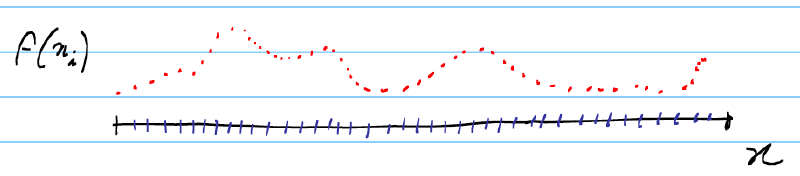
\includegraphics[width=0.6\linewidth]{fig4.png}
\end{figure}
\begin{equation}
    \Braket{i | v} = v_i, \quad \Braket{x|f} = f(x) \quad \text{($x$ is equivalent to the index of the component)}
\end{equation}
For ``well-behaved'' functions(``square-integrable'') can define an inner product:
\begin{equation}
    \Braket{f|g} = \int dx f^* (x) g(x)
\end{equation}
In particular $f(x)$ can be seen as the ``component'' od $\ket{f}$ along the base vector $\ket{x}$:
\begin{equation}
    f(x) = \Braket{x|f} \quad \text{where }\Braket{x|x'} = \delta(x-x')
\end{equation}
It is said ``delta function normalization''.

\noindent
Completeness relation in continuous dimensions: given the ket $\ket{f}$
\begin{equation}
    \Braket{x|f} = f(x) = \int dx' f(x') \delta{(x-x')} = \int dx' \Braket{x'|f}\Braket{x|x'} = \bra{x} \int dx' \ket{x'} \Braket{x' |f} = \bra{x} \mathds{1} \ket{f}
\end{equation}
Then,
\begin{equation}
    \boxed{\int dx \ket{x}\bra{x} = \mathds{1}}
\end{equation}
Define the dot product:
\begin{equation}
    \Braket{v|u} = \bra{v} \int dx \ket{x} \Braket{x|u} = \int dx \Braket{v|x} \Braket{x|u} = \int dx \Braket{x|v}^* \Braket{x|u} = \int dx v^* (x) u(x)
\end{equation}
\newpage

\noindent
then Hermiticity of $\mathcal{L}$ means:
\begin{equation}
    \bra{v} \mathcal{L} \ket{u} = \Braket{v|\mathcal{L}u} = \Braket{\mathcal{L}^{\dagger} v|u} = \Braket{\mathcal{L} v|u} = \Braket{u|\mathcal{L}v}^* = \bra{u} \mathcal{L} \ket{v}^*
\end{equation}
in other words:
\begin{equation}
    \mathcal{L}^\dagger = \mathcal{L}
\end{equation}
the operator $\mathcal{L}$ is local, i.e.:
\begin{equation}
    \bra{x'}\mathcal{L} \ket{x}  = \mathcal{L}(x) \delta{(x-x')}
\end{equation}
so, explicitly, the matrix elements of $\mathcal{L}$ are given by
\begin{equation}
    \Braket{v | \mathcal{L} | u}
= \bra{v} \underbrace{ \int \Ket{x'} \Bra{x'} }_{\text{completeness}} \mathcal{L} \underbrace{\int \Ket{x} \Bra{x} }_{\text{completeness}}  \ket{u}
\end{equation}
\begin{equation}
    = \int \! dx' \, dx \, v^*(x') \, \mathcal{L}(x) \, \delta(x - x') \, u(x)
= \int \! dx \, v^*(x) \, \mathcal{L}(x) \, u(x)
\end{equation}
so Hermiticity of $\mathcal{L}$ means:
\begin{equation}
    \Braket{v|\mathcal{L} u} = \Braket{\mathcal{L}v|u} \ \Rightarrow \ \int dxv^*(x) \mathcal{L}(x) u(x) = \int dx (\mathcal{L}v)^* udx
\end{equation}
Digression: on how the equivalence between some differential equations and an eigenvalue problem can be directly tested with a computer...)

\noindent
Need to discretize differential operators. For instance:
\begin{equation}
    \frac{d^2 \psi}{dx^2}
\end{equation}
discretize the space interval:
\begin{equation}
    \Psi_i \equiv \Psi (x_i) \quad \epsilon = x_{i+1}-x_i
\end{equation}
\begin{figure}[h]
    \centering
    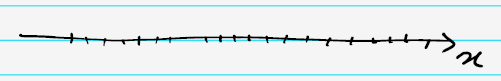
\includegraphics[width=0.7\linewidth]{fig5.png}
\end{figure}
\begin{equation}
    x_1, x_2, \cdots , x_N, \quad N \rightarrow \infty
\end{equation}
The trick is $N$ sufficiently large. But today a simple laptop can handle thousands of dimensions!

\vspace{3mm} \noindent
Approximate derivative with incremental ratio:
\begin{equation}
    \textcolor{red}{
\frac{d\psi}{dx}(x_i) \rightarrow \frac{\Psi_i - \Psi_{i-1}}{\epsilon}
\qquad\qquad
\frac{d\psi}{dx}(x_{i+1}) \rightarrow \frac{\Psi_{i+1} - \Psi_i}{\epsilon}
}
\end{equation}
the second derivative is just the incremental ratio of the incremental ratio:
\begin{equation}
    \textcolor{red}{
\frac{d^2 \psi}{dx^2}(x_i) 
\rightarrow \frac{\dfrac{d\Psi}{dx}(x_{i+1}) - \dfrac{d\Psi}{dx}(x_i)}{\epsilon}
= \frac{\dfrac{\Psi_{i+1} - \Psi_i}{\epsilon} - \dfrac{\Psi_i - \Psi_{i-1}}{\epsilon}}{\epsilon}
= \frac{\Psi_{i+1} - 2\Psi_i + \Psi_{i-1}}{\epsilon^2}
}
\end{equation}
Such operator can be written in matricial form:
\begin{equation}
    \textcolor{olive}{\frac{\Psi_{i+1} - 2\Psi_i + \Psi_{i-1}}{\epsilon^2}
= \sum_k \left[ \delta_{k,i+1} - 2\delta_{k,i} + \delta_{k,i-1} \right] \Psi_k
= \sum_k D_{i,k} \Psi_k }
\end{equation}

\newpage

\noindent
the matrix corresponding to the Kronecker delta is just the identity:
\begin{equation}
\textcolor{blue}{\delta_{i,k} =
\begin{bmatrix}
1 & 0 & 0 & \cdots & 0 \\
0 & 1 & 0 & \cdots & 0 \\
0 & 0 & 1 & \cdots & 0 \\
\vdots & \vdots & \vdots & \ddots & \vdots \\
0 & 0 & 0 & \cdots & 1
\end{bmatrix}}
\end{equation}
while in the other two matrices the diagonal with ones is ``shifted up or down'' one position:
\begin{equation}
    \textcolor{blue}{
\delta_{i-1,k} =
\begin{bmatrix}
0 & 0 & 0 & \cdots & 0 & 0 \\
1 & 0 & 0 & \cdots & 0 & 0 \\
0 & 1 & 0 & \cdots & 0 & 0 \\
0 & 0 & 1 & \cdots & 0 & 0 \\
\vdots & \vdots & \vdots & \ddots & \vdots & \vdots \\
0 & 0 & 0 & \cdots & 1 & 0
\end{bmatrix}
\quad
\delta_{i+1,k} =
\begin{bmatrix}
0 & 1 & 0 & \cdots & 0 & 0 \\
0 & 0 & 1 & \cdots & 0 & 0 \\
\vdots & \vdots & \vdots & \ddots & \vdots & \vdots \\
0 & 0 & 0 & \cdots & 1 & 0 \\
0 & 0 & 0 & \cdots & 0 & 1 \\
0 & 0 & 0 & \cdots & 0 & 0
\end{bmatrix}
}
\end{equation}
So the second derivative can be written as:
\begin{equation}
    \textcolor{blue}{
D = \frac{1}{\epsilon^2}
\left\{
\begin{bmatrix}
0 & 0 & 0 & \cdots & 0 & 0 \\
1 & 0 & 0 & \cdots & 0 & 0 \\
0 & 1 & 0 & \cdots & 0 & 0 \\
\vdots & \vdots & \vdots & \ddots & \vdots & \vdots \\
0 & 0 & 0 & \cdots & 1 & 0
\end{bmatrix}
- 2
\begin{bmatrix}
1 & 0 & 0 & \cdots & 0 \\
0 & 1 & 0 & \cdots & 0 \\
\vdots & \vdots & \ddots & \ddots & \vdots \\
0 & 0 & \cdots & 1 & 0 \\
0 & 0 & \cdots & 0 & 1
\end{bmatrix}
+
\begin{bmatrix}
0 & 1 & 0 & \cdots & 0 & 0 \\
0 & 0 & 1 & \cdots & 0 & 0 \\
\vdots & \vdots & \vdots & \ddots & \vdots & \vdots \\
0 & 0 & 0 & \cdots & 0 & 1 \\
0 & 0 & 0 & \cdots & 0 & 0
\end{bmatrix}
\right\}
}
\end{equation}
example: stationary Schrodinger equation:
\begin{equation}
    \textcolor{orange}{
\left[
-\frac{\hbar^2}{2m} \frac{d^2}{dx^2} + V(x)
\right] \Psi = E \Psi
}
\qquad
V(x) = \frac{1}{2} \omega^2 x^2
\end{equation}
In python just a few lines of code...
\begin{figure}[h]
    \centering
    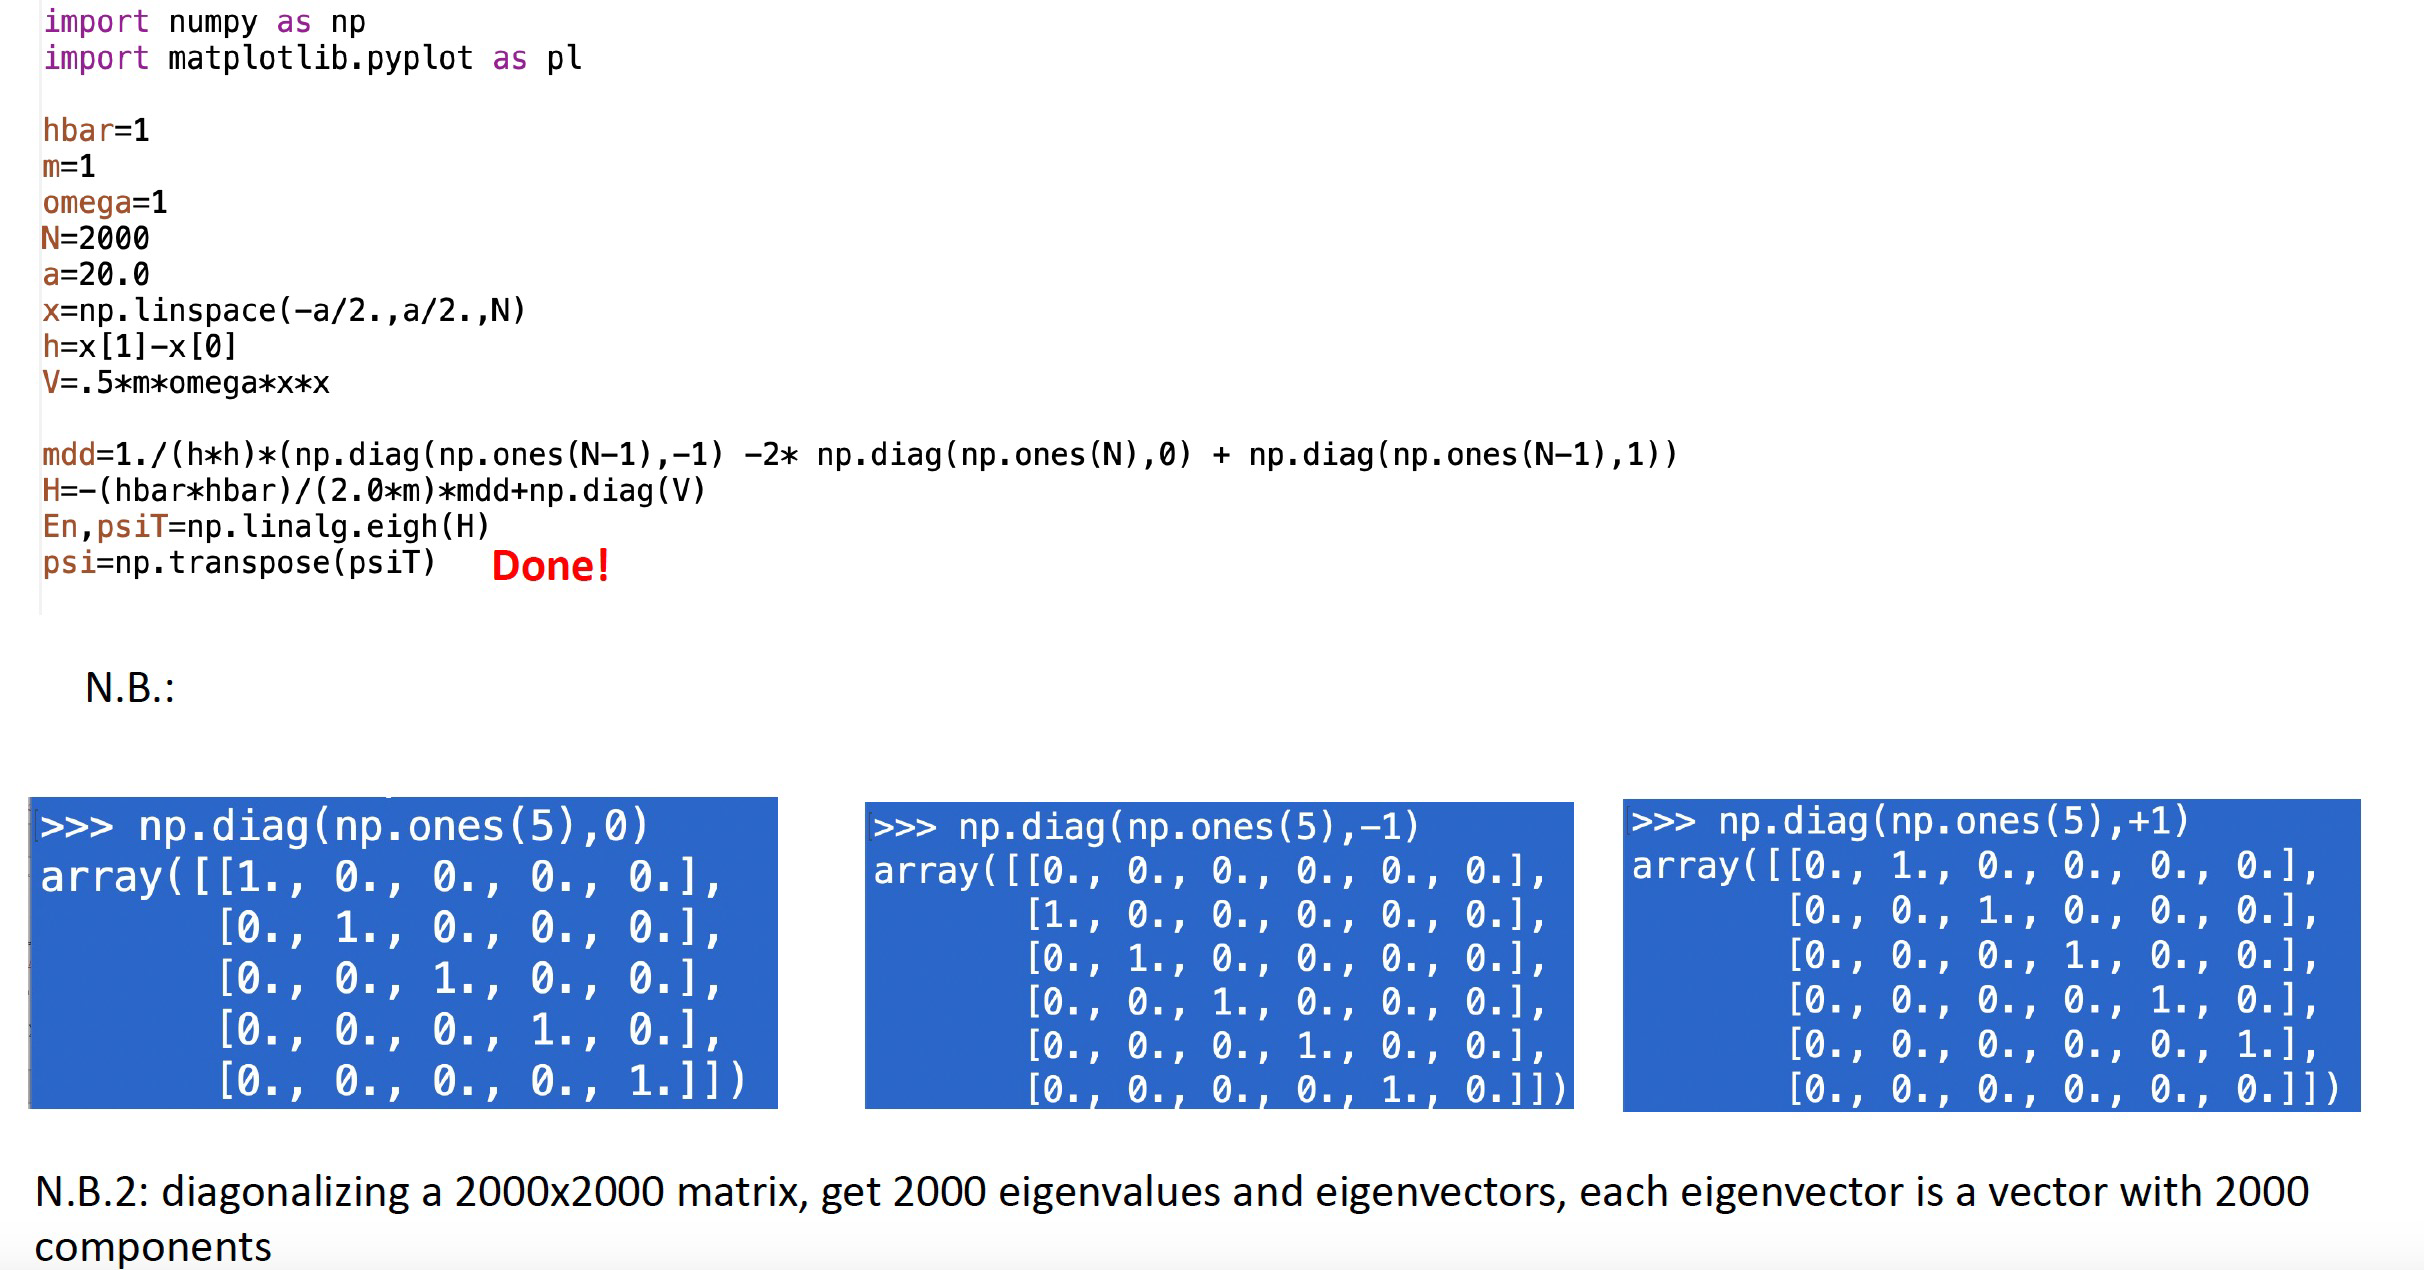
\includegraphics[width=1\linewidth]{fig6.png}
\end{figure}
\newpage

\noindent
A huge amount of energy levels (2000!):
\begin{equation}
    \textcolor{purple}{
E_n = \hbar \omega \left(n + \frac{1}{2} \right)
\rightarrow 
\frac{1}{2} \hbar \omega, \quad \frac{3}{2} \hbar \omega, \quad \ldots, \quad \frac{2000}{2} \hbar \omega
}
\end{equation}
it works!
\begin{figure}[h]
    \centering
    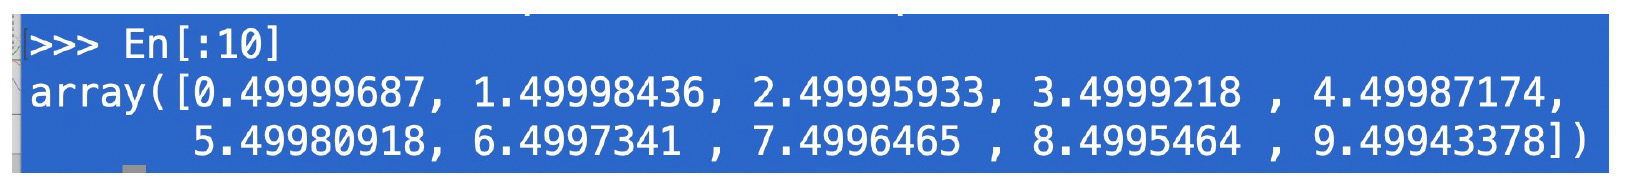
\includegraphics[width=0.8\linewidth]{fig7.png}
\end{figure}

\noindent
The Hermiticity condition for the differential operator:
\begin{equation}
    \mathcal{L} = p_0(x) \frac{d^2}{dx^2} + p_1(x) \frac{d}{dx} + p_2(x)
\end{equation}
is that:
\begin{equation}
    p_0' (x) = p_1 (x)
\end{equation}
in this way the operator simplifies:
\begin{equation}
    \mathcal{L} = p_0(x) \frac{d^2}{dx^2} + p_1(x) \frac{d}{dx} + p_2(x) = \frac{d}{dx}\left( p_0 (x) \frac{d}{dx} \right) + p_2 (x) \quad \color{olive} (\text{then } \mathcal{L}u = (p_0 u')' + p_2u) \color{black}
\end{equation}
check that is true: Hermiticity of $\mathcal{L}$ (assume $p_0 = p_0 ^*$)
\begin{equation}
    \int_a^b v^*(x)\, \mathcal{L}u(x)\, dx
= \int_a^b \left[ (\rho_0 v^*)' u + v^* \rho_2 u \right] dx
\end{equation}
\textbf{N.B. }The Hilbert space is defined in the $[a,b]$ interval. The boundary conditions in $x=a$ and $x=b$ will be fundamental for the Hermiticity!

\noindent
Integrate by parts twice:
\begin{align*}
    \int_a^b v^* \mathcal{L}u\, dx 
&= \left[ v^* p_0 u' \right]_a^b 
+ \int_a^b \left[ -(v^*)' p_0 u' + v^* p_2 u \right] dx \\
&= \left[ v^* p_0 u' - (v^*)' p_0 u \right]_a^b 
+ \int_a^b \left[ \left( p_0 (v^*)' \right)' u + v^* p_2 u \right] dx \\
&= \left[ v^* p_0 u' - (v^*)' p_0 u \right]_a^b 
+ \int_a^b \left[ \left( p_0 v' \right)'^* + p_2 v^* \right] u\, dx \\
&= \left[ v^* p_0 u' - (v^*)' p_0 u \right]_a^b 
+ \int_a^b \left( \mathcal{L}^* v \right)^* u\, dx \quad (\text{where } \ \mathcal{L}^* v = \left( p_0 v' \right)' + p_2 v)
\end{align*}
So, indeed, the condition $p_0’(x)=p_1(x)$ in the linear operator:
\begin{equation}
    \mathcal{L}(x) = p_0(x) \frac{d^2}{dx^2} + p_1(x) \frac{d}{dx} + p_2(x)
\end{equation}
guarantees that $\mathcal{L}$ is Hermitian provided that:
\begin{equation}
    \left[ v^* \rho_0 u' - (v^*)' \rho_0 u \right]_a^b = 0
\end{equation}
which implies vanishing boundary conditions for $u,v,u’$ and $v’$:
\begin{equation}
    u(a) = u(b) = u'(a) = u'(b) = v(a) = v(b) = v'(a) = v'(b) = 0
\end{equation}
\newpage
\noindent
In particular, if $u$ and $v$ are eigenfunctions of $\mathcal{L}$ with (real) eigenvalues $\lambda_u$ and $\lambda_v$:
\begin{align}
        &\quad \ \ \left[ p_0 \left( v^{*} u' - (v^{*})' u \right) \right]_a^b = 
\Braket{v | \mathcal{L} | u} - \Braket{\mathcal{L} v | u} 
= \lambda_u \Braket{v | u} - \lambda_v \Braket{v | u}\\
&\Rightarrow \left( \lambda_u - \lambda_v \right)
\int_a^b v^*(x) u(x)\, dx
= \left[ p_0 \left( v^* u' - (v^*)' u \right) \right]_a^b = 0
\end{align}
so if the boundary conditions are verified and $\lambda_u \neq \lambda_v$ one has $\Braket{v|u} = 0$, i.e. eigenvectors corresponding to different eigenvalues are orthogonal.

\noindent
In many physical problems the operator is self-adjoint by construction (think about QM). In some other cases it is not, but there is a way to find a function $w(x)$ so that $w(x)\mathcal{L}$ is Hermitian!

\noindent
Then the Sturm-Liouville eigenvalue problem becomes:
\begin{equation}
    w(x)\, \mathcal{L}(x)\, \psi(x) = w(x)\, \lambda\, \psi(x)
\end{equation}
where $\lambda$ and $\psi$ are the same of the original problem. The correct choice for $w(x)$ is:
\begin{equation}
    w(x) = \frac{1}{p_0(x)} \exp\left( \int^x \frac{p_1(x')}{p_0(x')} \, dx' \right)
\end{equation}
direct substitution:
\begin{align*}
    w(x) \mathcal{L}(x) &= \frac{1}{p_0} e^{\int \frac{p_1}{p_0} \, dx}
\left[ 
p_0 \frac{d^2}{dx^2} + p_1 \frac{d}{dx} + p_2 
\right]\\
&= \left[
e^{\int \frac{p_1}{p_0} \, dx} \frac{d^2}{dx^2}
+ \frac{p_1}{p_0} e^{\int \frac{p_1}{p_0} \, dx} \frac{d}{dx}
+ \frac{p_2}{p_0} e^{\int \frac{p_1}{p_0} \, dx}
\right]\\
&= \bar{p}_0 \frac{d^2}{dx^2} + \bar{p}_1 \frac{d}{dx} + \bar{p}_2
\end{align*}
with
\begin{equation*}
    \bar{p}_0 = e^{\int \frac{p_1}{p_0} \, dx} \quad \bar{p}_1 = \frac{p_1}{p_0} e^{\int \frac{p_1}{p_0} \, dx} \quad \bar{p}_2 = \frac{p_2}{p_0}e^{\int \frac{p_1}{p_0} \, dx}
\end{equation*}
the new operator is Hermitian because:
\begin{equation}
    \color{red} \bar{p_0}' = \frac{p_1}{p_0}e^{\int \frac{p_1}{p_0} \, dx} = \bar{p_1} \color{black}
\end{equation}

\noindent
\textbf{Important}

\noindent
The Hermiticity condition for $w\mathcal{L}$ now reads (\textbf{N.B.}: $w(x)$ is real):
\begin{equation}
    \int_a^b v^*(x)\, w(x)\, \mathcal{L} u(x)\, dx
=
\left[
w \left(v^* \bar{p_0} u' - (v^*)' \bar{p_0} u \right)
\right]_a^b
+
\int_a^b w(x)\, (\mathcal{L} v)^*\, u\, dx
\end{equation}
if the boundary term vanishes the Hermiticity condition becomes:
\begin{equation}
    \int_a^b v^*(x)\, \mathcal{L} u(x)\, \underbrace{w(x)\, dx}
=
\int_a^b \left( \mathcal{L} v \right)^* u(x)\, \underbrace{w(x)\, dx}
\end{equation}
we can now generalize the definition of the scalar product (the new definition does not alter any of its required properties):
\begin{equation}
    \color{red} \Braket{v | u} \equiv \int_a^b v^*(x)\, u(x)\, w(x)\, dx \quad 
    \color{olive} w(x) = \text{weight function} \color{black}
\end{equation}
with the new definition of the scalar product the hermiticity condition implies:
\begin{equation}
    \int_a^b v^*(x)\, \mathcal{L} u(x)\, w(x)\, dx 
- \int_a^b \left(\mathcal{L} v\right)^* u(x)\, w(x)\, dx 
= (\lambda_u - \lambda_v) \int_a^b v^*(x)\, u(x)\, w(x)\, dx 
= \left[ w\, p_0 \left(v^* u' - (v^*)' u\right) \right]_a^b = 0
\end{equation}
so if $\lambda_u \neq \lambda_v$ the two eigenfunctions are orthogonal with the new definition of the scalar product.
\newpage

\noindent
\textbf{Summarizing:}
\begin{itemize}
    \item if the second-order differential operator $\mathcal{L}$ satisfies the condition $p_0’=p_1$ it is Hermitian under a scalar product with uniform weight ($w(x)=1$) and vanishing boundary conditions:
    \begin{equation}
        \left[ p_0 \left( v^* u' - (v^*)' u \right) \right]_a^b = 0
    \end{equation}
    \item If instead $p_0’\neq p_1$ introduce the weight function:
    \begin{equation}
        w(x) = \frac{1}{p_0(x)} \exp\left( \int \frac{p_1}{p_0} \, dx \right)
    \end{equation}
    \item and $\mathcal{L}$ is Hermitian under a new scalar product with weight $w(x)$, i.e.
    \begin{equation}
        \Braket{v|u} = \int v^* u\, w\, dx
    \end{equation}
    and boundary conditions:
    \begin{equation}
        \left[ w p_0 \left( v^* u' - (v^*)' u \right) \right]_a^b = 0
    \end{equation}
\end{itemize}

\noindent
\textbf{Example \#1 (Laguerre equation)}
\begin{equation}
    \mathcal{L} = x \frac{d^2}{dx^2} + (1 - x) \frac{d}{dx}
= p_0 \frac{d^2}{dx^2} + p_1 \frac{d}{dx} + p_2
\end{equation}
In this case, $p_0 = x$, $p_1 = 1-x$, $p_2 = 0$. Then,
\begin{equation}
    p_0' = 1 \neq p_1 \quad \Rightarrow \quad \color{red} \text{$\mathcal{L}$ is not hermitian!} \color{black}
\end{equation}
construct the weight function:
\begin{equation}
    w(x) = \frac{1}{p_0} \exp{\int\frac{p_1}{p_0}dx} = \frac{1}{x} \exp{\int \frac{1-x}{x}dx } = \frac{1}{x} e^{\ln x - x}
= \frac{1}{x} x e^{-x}= e^{-x}
\end{equation}
then the boundary conditions are:
\begin{equation}
    \left[ w_0 \left( v^{*} u' - (v^{*})' u \right) \right]_{a}^{b}
= \left[ x e^{-x} \left( v^{*} u' - (v^{*})' u \right) \right]_{0}^{\infty} = 0
\end{equation}
and the operator $\mathcal{L}$ is Hermitian under the scalar product:
\begin{equation}
    \Braket{v|u} = \int_0 ^\infty v^* (x) u(x) e^{-x} dx
\end{equation}
\noindent
\textbf{Example \#2 (Legendre equation)}
\begin{equation}
    \mathcal{L} y(x) = -(1-x^2) y''(x) + 2xy'(x) = \lambda y(x)
\end{equation}
In this case, $p_0 = x^2-1$, $p_1 = 2x$. Then,
\begin{equation}
    p_0' = 2x = p_1 \quad \Rightarrow \quad \color{red} \text{self-adjoint} \color{black}
\end{equation}
arises when the Laplacian operator $\Delta = \nabla^2$ is written in polar coordinates. Look for non-singular solutions in the interval $-1 \leq x \leq 1$ (\textbf{N.B.} at boundaries the ODE is singular!).

\noindent
use Frobenius procedure:
\begin{equation}
    y = \sum_{j=0}^\infty a_j x^{s+j} \quad \text{(expansion in $x=0$)}
\end{equation}

\newpage
\noindent
in standard form the equation is:
\begin{equation}
    \frac{d^2y}{dx^2} + P(x) \frac{dy}{dx} + Q(y) y = 0
\end{equation}
with
\begin{equation}
    P(x) = -\frac{2x}{1-x^2} \quad Q(x) = \frac{\lambda}{1-x^2}
\end{equation}
has indicial equation:
\begin{equation}
    s(s-1) + p_0 s + q_0 = 0
\end{equation}
with
\begin{equation}
    \begin{cases}
        \lim_{x \rightarrow x_0} P(x) (x-x_0) = p_0 = 0 \\
        \lim_{x \rightarrow x_0} Q(x) (x-x_0)^2 = q_0 = 0 
    \end{cases} \quad \Rightarrow \quad s(s-1) = 0 \quad \Rightarrow \quad \begin{cases}
        s=0 \\ s=1
    \end{cases}
\end{equation}
solutions with $s=0$

\noindent
plug series with $s=0$ in the differential equation to get a recursive relation for the coefficients $a_k$
\begin{equation}
    y = \sum_{k=0}^{\infty} a_k x^k \qquad y' = \sum_{k=0}^{\infty} k a_k x^{k-1} \qquad   y'' = \sum_{k=0}^{\infty} k(k-1) a_k x^{k-2} \\
\end{equation}
\begin{equation}
    -(1 - x^2) \sum_{k=0}^{\infty} k(k-1) a_k x^{k-2}
+ 2x \sum_{k=0}^{\infty} k a_k x^{k-1}
- \lambda \sum_{k=0}^{\infty} a_k x^k = 0
\end{equation}
set $k \rightarrow k+2$ here to get same power of $x$ everywhere
\begin{equation*}
    - \sum_k k(k-1) a_k x^{k-2}
+ \sum_k k(k-1) a_k x^k
+ 2 \sum_k k a_k x^k
- \lambda \sum_k a_k x^k
\end{equation*}
\begin{equation}
    \sum_k \left[ \underbrace{
-(k+2)(k+1) a_{k+2}
+ k(k-1) a_k
+ 2k a_k
- \lambda a_k}_{\color{red}\text{this term must vanish $\rightarrow$ get recursive relation between $a_k$ and $a_{k+2}$}}
\right] x^k = 0
\end{equation}
then:
\begin{equation}
    -(k+2)(k+1) a_{k+2}
+ k(k-1) a_k
+ 2k a_k
- \lambda a_k = 0
\end{equation}
\begin{equation}
    a_{k+2} = \frac{k(k+1) - \lambda}{(k+1)(k+2)} a_k
\end{equation}
can set $a_1=0$, so for $s=0$ only $k=$odd number appear. The series diverges unless it is truncated at some $k$ (i.e. instead of a series, the solutions must be polynomials).

\noindent
Set $\lambda = l(l+1)$ when $l =$ even integer. Then:
\begin{equation}
    a_{l+2} = \frac{l(l+1) - l(l+1)}{(l+1)(l+2)} a_l = 0
\end{equation}
and also $a_{l+4}, a_{l+6}, a_{l+8},$ etc will vanish.

\noindent
Eventually, the overall set of eigenfunctions will be polynomials of all integer degrees $l$ (Legendre polynomials). Since $\mathcal{L}$ is Hermitian Legendre polynomials are orthogonal with unit weight in the interval $(-1,1)$.

\noindent
\textbf{Example \#3 (Hermite equation)}
\begin{equation}
    \mathcal{L} y = -y'' +2xy' =\lambda y \quad 0 \leq x \leq \infty
\end{equation}
In this case, $p_0 = -1$, $p_1 = 2x $. Then,
\begin{equation}
    p_0 ' = 0 \neq p_1 \quad \Rightarrow \quad \mathcal{L}\text{ is not Hermitian}
\end{equation}
find weight equation:
\begin{equation}
    W(x) = \frac{1}{p_0} \exp{\int \frac{p_1}{p_0} \, dx}
= \frac{1}{-1} \exp{\int \frac{2x}{-1} \, dx} = - e^{-x^2} \Rightarrow W(x) = e^{-x^2}
\end{equation}
so $\mathcal{L}$ is Hermitian under the definition of the scalar product:
\begin{equation}
    \Braket{f | g} = \int_{-\infty}^{+\infty} f^*(x)\, g(x)\, e^{-x^2} \, dx
\end{equation}
use Frobenius method looking for a series of the form:
\begin{equation}
    y(x) = \sum_{k=0}^{\infty} a_k x^{s + k}
\end{equation}
indicial equation:
\begin{equation}
    \begin{cases}
        P(x) = -2x \\ Q(x) = \lambda
    \end{cases} \ \  \Rightarrow \ \ \begin{cases}
        p_0 = \lim_{x \rightarrow 0} xP(x) = 0 \\
        q_0 = \lim_{x \rightarrow 0} x^2 Q(x) = 0
    \end{cases} \ \ \Rightarrow \ \ s(s-1) = 0 \ \ \Rightarrow \ \ \begin{cases}
        s=0 \\ s=1
    \end{cases}
\end{equation}
solution with $s=0$
\begin{equation}
    y = \sum_{k=0}^{\infty} a_k x^k \qquad y' = \sum_{k=0}^{\infty} k a_k x^{k-1} \qquad   y'' = \sum_{k=0}^{\infty} k(k-1) a_k x^{k-2} \\
\end{equation}
plug in ODE
\begin{align*}
& \quad \ - \sum_k k(k-1) a_k x^{k-2}
+ 2x \sum_k k a_k x^{k-1}
- \lambda \sum_k a_k x^k = 0 \\
\\
& \Rightarrow - \sum_k k(k-1) a_k x^{k-2} + 2 \sum_k k a_k x^k
- \lambda \sum_k a_k x^k = 0\\
&\Rightarrow 
\sum_k \left[
-(k+2)(k+1) a_{k+2}
+ 2k a_k
- \lambda a_k
\right] x^k = 0\\
&\Rightarrow 
a_{k+2} = \frac{2k - \lambda}{(k+1)(k+2)} a_k
\end{align*}
the series converges for all $x$ but behaves as $\exp(x^2)$ for large $|x|$ so it has no finite norm (even with weigth $\exp(x^2)$) $\Rightarrow$ need to truncate the series setting $\lambda = 2k$ (even polynomial). For $s=1$ we obtain odd polynomials. $\Rightarrow$ \color{red} Hermite polynomials at all integer $\lambda$. \color{black}

\vspace{3mm}\noindent
\textbf{Summary of Sturm-Liouville theory}
\begin{itemize}
    \item A second-order differential operator is Hermitian if it is self-adjoint in the differential equation sense and the functions on which it operates are required to satisfy appropriate boundary conditions. In that event, the scalar product consistent with Hermiticity is an unweighted integral over the range between its boundaries.
    \item If a second-order differential operator is not self-adjoint in the differential-equation sense, it will nevertheless be Hermitian if it satisfies appropriate boundary conditions and if the scalar product includes the weight function that makes the original differential equation self-adjoint.
    \item A Hermitian operator on a Hilbert space has a complete set of eigenfunctions. Thus, they span the space and can be used as basis for an expansion.
    \item The eigenvalues of a Hermitian operator are real.
    \item The eigenfunctions of a Hermitian operator corresponding to different eigenvalues are orthogonal, using the appropriate scalar product.
    \item Degenerate eigenfunctions of a Hermitian operator can be orthogonalized using the Gram-Schmidt or any other orthogonalization process.
\end{itemize}

\newpage

\section{Handout 04}

\large
\begin{center}
    \textbf{Complex variable theory}
\end{center}

\normalsize
\noindent
\begin{itemize}
    \item Many physical problems are better solved using complex numbers.
    \item Some of them are intrinsically defined in the complex plane.(Schrodinger equation contains explicitly the imaginary unit!)
    \item Analytic continuation of functions of real variable to the complex plane allows to gain a grater insight on their properties
    \item Complex solutions allow to see the transition from exponential to oscillatory behaviors in systems that can have both.
    \item Some real integrals can be solved by extending them to the complex plane.
    \item Many physical quantities originally real become complex when the theory is extended. The mass of a particle acquires an imaginary part when the particle is unstable and has a finite lifetime. A real index of refraction becomes complexs when the effect of absorption is included.
\end{itemize}

\noindent
To do calculus in the complex plane we need first to extend the definition of derivative In this chapter we will be interested to analytic functions, i.e. single-valued functions which are differentiable in a region of the complex plane.


\vspace{2mm} \noindent
\textbf{Derivatives in the complex plane}

\noindent
A big difference between derivatives on the real axis and on the complex plane is that in the complex plane the same point $z_0$ can be approached along an infinite number of different paths:
\begin{figure}[h]
    \centering
    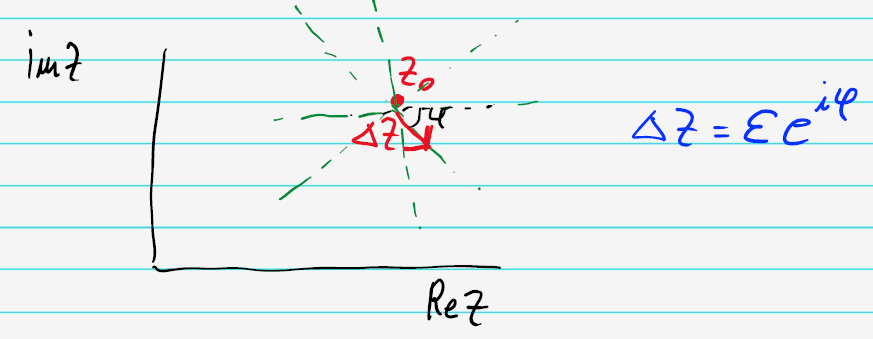
\includegraphics[width=0.6\linewidth]{fig8.png}
\end{figure}
in principle along each different path the derivative is different:
\begin{equation}
\left.     \frac{df}{dz} \right|_{z_0}
= \lim_{z \to z_0} \frac{f(z_0 + \Delta z) - f(z_0)}{\Delta z}
= \lim_{\varepsilon \to 0} \frac{f(z_0 + \varepsilon e^{i\varphi}) - f(z_0)}{\varepsilon e^{i\varphi}}
\end{equation}
does the result depend on the approaching angle $\phi$? If not, the function is \textbf{differentiable}.

\vspace{2mm} \noindent
\textbf{Cauchy-Riemann conditions}

\noindent
Let’s write explicitly a function $f(z)$ in components:
\begin{equation}
    z=x+iy, \quad dz = dx + idy, \quad f(z) = f(x+iy) = u(x,y)+iv(x,y)
\end{equation}
we can perform the derivative along the real axis:
\begin{equation}
    dz=dx \quad (dy=0)
\end{equation}

\newpage
\begin{figure}[h]
    \centering
    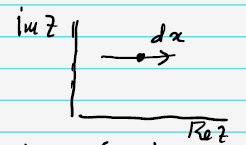
\includegraphics[width=0.25\linewidth]{fig9.png}
\end{figure}
\begin{equation}
    \frac{d f}{d z}
= \frac{u(x + dx, y) + i v(x + dx, y) - u(x, y) - i v(x, y)}{dx}
= \frac{\partial u}{\partial x} + i \frac{\partial v}{\partial x}
\end{equation}
or do the same along the imaginary axis:
\begin{equation}
    dz=idy \quad (dx=0)
\end{equation}
\begin{figure}[h]
    \centering
    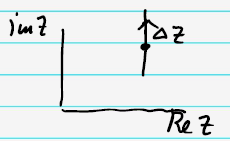
\includegraphics[width=0.25\linewidth]{fig10.png}
\end{figure}
\begin{equation}
    \frac{d f}{d z}
= \frac{u(x, y + dy) + i v(x, y + dy) - u(x, y) - i v(x, y)}{i \, dy}
= \frac{1}{i} \left( \frac{\partial u}{\partial y} + i \frac{\partial v}{\partial y} \right)
= \frac{\partial v}{\partial y} - i \frac{\partial u}{\partial y}
\end{equation}
So, along the two different paths we found two different results. the derivative is unique and the function is differentiable if the two expressions coincide:
\begin{equation}
    \frac{\partial u}{\partial x} + i \frac{\partial v}{\partial x}
= \frac{\partial v}{\partial y} - i \frac{\partial u}{\partial y} \quad \Rightarrow \quad \color{red} \boxed{\frac{\partial u}{\partial x} = \frac{\partial v}{\partial y} \ , \ \frac{\partial u}{\partial y} = -\frac{\partial v}{\partial x}} \quad \textbf{Cauchy-Riemann conditions} \color{black}
\end{equation}
Is this requirement a strong one? turns out it is not, i.e. most of the functions that we are familiar to comply to the Cauchy-Riemann conditions and are differentiable.

\noindent
take an integer power of $z$: ($n \in \mathbb{Z}$)
\begin{equation}
    f(z) = z^n , \quad dz = \varepsilon e^{i \varphi}
\end{equation}
\begin{figure}[h]
    \centering
    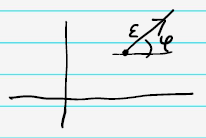
\includegraphics[width=0.25\linewidth]{fig11.png}
\end{figure}
\begin{equation}
    \frac{d f}{d z}
= \lim_{\varepsilon \to 0} \frac{(z + \varepsilon e^{i\varphi})^n - z^n}{\varepsilon e^{i\varphi}}
\end{equation}
we can extend the binomial in the usual way, keeping only the linear term in $\varepsilon$:
\begin{equation}
    \left( z + \varepsilon e^{i\varphi} \right)^n
= \sum_{k=0}^{n} \binom{n}{k} z^k \left( \varepsilon e^{i\varphi} \right)^{n - k}
= z^n + n z^{n-1} \varepsilon e^{i\varphi} + \mathcal{O}(\varepsilon^2)
\end{equation}
substituting in the limit, the dependence on the approaching angle $\phi$ cancels:
\begin{equation}
    \frac{d f}{d z}
= \lim_{\varepsilon \to 0} \frac{\cancel{z^n} + n z^{n-1} \varepsilon e^{i\varphi} \cancel{- z^n}}{\varepsilon e^{i\varphi}}
= \lim_{\varepsilon \to 0} \frac{n z^{n-1} \cancel{\varepsilon e^{i\varphi}}}{\cancel{\varepsilon e^{i\varphi}}}
= n z^{n-1} \quad (\text{familiar result})
\end{equation}
\newpage

\noindent
In the complex plane transcendental functions are defined by their power series:
\begin{align}
    \exp(z) &= \sum_{m=0}^{\infty} \frac{z^m}{m!}
= 1 + z + \frac{z^2}{2!} + \frac{z^3}{3!} + \cdots\\
\sin(z) &= \sum_{m=0}^{\infty} (-1)^m \frac{z^{2m+1}}{(2m+1)!}
= z - \frac{z^3}{3!} + \frac{z^5}{5!} - \cdots\\
\cos(z) &= \sum_{m=0}^{\infty} (-1)^m \frac{z^{2m}}{(2m)!}
= 1 - \frac{z^2}{2!} + \frac{z^4}{4!} - \cdots\\
\ln(1+z) &= \sum_{m=0}^{\infty} (-1)^m \frac{z^{m+1}}{m+1}
= z - \frac{z^2}{2} + \frac{z^3}{3} - \cdots
\end{align}
$\ln (1+z)$ is ``polydronic'' in $z=-1$.

\noindent
If a series converges its derivative is the sum of the derivatives of its terms, so all transcendental functions are differentiable (if single-valued) because they are sums of differentiable powers of $z$.

\noindent
Cauchy-Riemann conditions are not only necessary for differentiability, but also sufficient (i.e. if they are verified the derivative exists)
\begin{equation}
    \delta f 
= \left( \frac{\partial u}{\partial x} + i \frac{\partial v}{\partial x} \right) \delta x 
+ \left( \frac{\partial u}{\partial y} + i \frac{\partial v}{\partial y} \right) \delta y
\end{equation}
use Cauchy-Riemann in the second parenthesis:
\begin{align*}
    \delta f &= 
\left( \frac{\partial u}{\partial x} + i \frac{\partial v}{\partial x} \right) \delta x
+ \left( -\frac{\partial v}{\partial x} + i \frac{\partial u}{\partial x} \right) \delta y \\
&=
\left( \frac{\partial u}{\partial x} + i \frac{\partial v}{\partial x} \right) \delta x
+ \left( i \frac{\partial v}{\partial x} + \frac{\partial u}{\partial x} \right) i \delta y \\
&=
\left( \frac{\partial u}{\partial x} + i \frac{\partial v}{\partial x} \right)
\left( \delta x + i \delta y \right)
= \left( \frac{\partial u}{\partial x} + i \frac{\partial v}{\partial x} \right) \delta z \\
&\Rightarrow \frac{d f}{d z} = \frac{\partial u}{\partial x} + i \frac{\partial v}{\partial x} \quad \color{red} \text{does not depend on the direction of $dz$} \color{black}
\end{align*}

\vspace{3mm}
\begin{center}    
\noindent
\textbf{analytic functions}: differentiable and single-valued

\noindent
\textbf{entire functions}: analytic in all the complex plane

\noindent
\textbf{singular point}: a point where the derivative does not exist
\end{center}

\noindent
For real functions the derivative is a local property, i.e. it only provides information about the function in the neighborhood of a point. In the complex plane differentiability has more consequences. consider the Cauchy-Riemann conditions:
\begin{equation}
    \left\{
\begin{aligned}
\frac{\partial u}{\partial x} &= \frac{\partial v}{\partial y} \\
\frac{\partial u}{\partial y} &= -\frac{\partial v}{\partial x}
\end{aligned}
\right.
\quad
\textcolor{blue}{\text{differentiate}}
\quad
\left\{
\begin{aligned}
\frac{\partial^2 u}{\partial x^2} &= \frac{\partial^2 v}{\partial x \partial y} \\
\frac{\partial^2 u}{\partial y^2} &= -\frac{\partial^2 v}{\partial y \partial x}
\end{aligned}
\right.
\end{equation}
since:
\begin{equation}
    \frac{\partial^2 v}{\partial x \partial y} = \frac{\partial^2 v}{\partial y \partial x}
\Rightarrow
\frac{\partial^2 u}{\partial x^2} = -\frac{\partial^2 u}{\partial y^2}
\Rightarrow
\boxed{
\frac{\partial^2 u}{\partial x^2} + \frac{\partial^2 u}{\partial y^2} = 0
} \quad \color{red}\text{(Laplace's equation)} \color{black}
\end{equation}
In the same way:
\begin{align}
    \left\{
\begin{aligned}
\frac{\partial v}{\partial x} &= -\frac{\partial u}{\partial y} \\
\frac{\partial v}{\partial y} &= \phantom{-}\frac{\partial u}{\partial x}
\end{aligned}
\right.
\quad
\textcolor{blue}{\text{differentiate}}
\quad
\left\{
\begin{aligned}
\frac{\partial^2 v}{\partial x^2} &= -\frac{\partial^2 u}{\partial x \partial y} \\
\frac{\partial^2 v}{\partial y^2} &= \phantom{-}\frac{\partial^2 u}{\partial y \partial x}
\end{aligned}
\right. \quad
\Rightarrow \quad
\boxed{
\frac{\partial^2 v}{\partial x^2} + \frac{\partial^2 v}{\partial y^2} = 0
}
\end{align}
The two functions $u$ and $v$ are referred to as harmonic functions.

\newpage
\noindent
Laplace’s equation in two dimensions enters in the calculation of electric fields:
\begin{equation}
    \begin{cases}
        \vec{E} = -\vec{\nabla} \varphi \\ 
        \vec{\nabla} \cdot \vec{E} = \rho
    \end{cases} \Rightarrow
\vec{\nabla}  (-\vec{\nabla} \varphi) = \rho
\Rightarrow
\nabla^2 \varphi = \frac{\partial^2 \varphi}{\partial x^2} + \frac{\partial^2 \varphi}{\partial y^2} = -\rho
\end{equation}
$\Phi = $ electric potential
\begin{figure}[h]
    \centering
    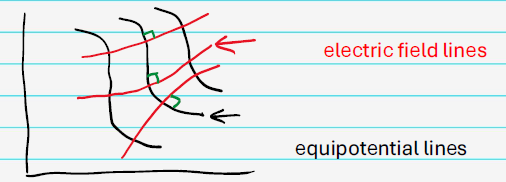
\includegraphics[width=0.5\linewidth]{fig12.png}
\end{figure}

\noindent
$\vec{E} = - \vec{\nabla} \varphi$ so $\vec{E}$ is perpendicular to the lines $\varphi (x,y) = $ constant

\noindent
Interestingly, if the function $f=u+iv$ is differentiable and $u$ and $v$ comply to Cauchy-Riemann conditions, also the lines $u(x,y)=$constant and $v(x,y)=$constant are perpendicular.

\noindent
If the point $x_0$,$y_0$ is on the curve $u(x,y)=c$ then also $x_0+\delta x$, $y_0+\delta y$ is on the curve if:
\begin{equation}
    \frac{\partial u}{\partial x} \, dx + \frac{\partial u}{\partial y} \, dy = 0
\Rightarrow
\left( \frac{dy}{dx} \right)_u = -\frac{\partial u / \partial x}{\partial u / \partial y} \quad \color{red}\text{slope of $u(x,y)=c$} \color{black}
\end{equation}
in the same way if the point $x_0$,$y_0$ is also on the curve $v(x,y)=k$ then also $x_0+\delta x$, $y_0+\delta y$ is on the curve if:
\begin{equation}
    \frac{\partial v}{\partial x} \, dx + \frac{\partial v}{\partial y} \, dy = 0
\Rightarrow
\left( \frac{dy}{dx} \right)_v = -\frac{\partial v / \partial x}{\partial v / \partial y}
= \frac{\partial u / \partial y}{\partial u / \partial x} \quad \text{(Cauchy-Riemann)}
\end{equation}
then:
\begin{equation}
    \left( \frac{\partial y}{\partial x} \right)_u
= -\frac{1}{\left( \frac{\partial y}{\partial x} \right)_v}D
\end{equation}
so the two slopes are orthogonal since:
\begin{equation}
    \frac{(dy)_u}{(dx)_u}
= -\frac{1}{\left( \frac{(dy)_v}{(dx)_u} \right)}
= -\frac{(dx)_u}{(dy)_v} \ \ \Rightarrow \ \ (dx)_u (dx)_v + (dy)_u (dy)_v = 0
\end{equation}
so, $(dx, dy)_u$ and $(dx, dy)_v$ are orthogonal. This means that if it is possible to identify the electric potential with the real part of an analytic function in the complex plane the imaginary part will automatically yield the electric field lines!

\vspace{2mm} \noindent
\textbf{Derivative of the logarithm}
\begin{equation}
    z = r e^{i(\varphi + 2n\pi)}
\quad \left(
r^2 = x^2 + y^2, \quad
\varphi + 2n\pi = \tan^{-1} \left( \frac{y}{x} \right)
\right)
\end{equation}
then:
\begin{equation}
    \ln z = \ln r + i(\varphi + 2n\pi) = u + iv
\Rightarrow
\left\{
\begin{aligned}
u &= \ln r \\
v &= \varphi + 2n\pi
\end{aligned}
\right.
\end{equation}
The logarithm is a polydromial function (infinite number of values). In order to make it single-valued one needs to impose additional conditions (cuts in the complex plane, more on that later). Anyway, let’s check if it complies with Cauchy-Riemann conditions:
\begin{equation}
    \frac{\partial u}{\partial x}
= \frac{1}{r} \frac{\partial r}{\partial x}
= \frac{1}{r} \cdot \frac{x}{r}
= \frac{x}{r^2}, \quad
\frac{\partial u}{\partial y}
= \frac{1}{r} \frac{\partial r}{\partial y}
= \frac{y}{r^2} \quad \frac{\partial v}{\partial x} = \frac{\partial \varphi}{\partial x} = -\frac{y}{r^2},
\quad
\frac{\partial v}{\partial y} = \frac{x}{r^2}
\end{equation}

\newpage
\noindent
so, indeed:
\begin{equation}
    \frac{\partial u}{\partial x} = \frac{\partial v}{\partial y},
\qquad
\frac{\partial u}{\partial y} = -\frac{\partial v}{\partial x}
\end{equation}
So with the exception of for $r=0$ where the function is not defined the logarithm is differentiable. Then:
\begin{equation}
    \frac{d \ln z}{d z}
= \frac{\partial u}{\partial x} + i \frac{\partial v}{\partial x}
= \frac{x}{r^2} - i \frac{y}{r^2}
= \frac{x - i y}{r^2}
= \frac{\cancel{z^*}}{z \cdot \cancel{z^*}}
= \frac{1}{z} \quad \text{(familiar rule of derivation)}
\end{equation} 
\textbf{Point at infinity}

\noindent
In complex variable theory, infinity is regarded as a single point, and behavior in its neighborhood is discussed after making a change of variable from $z$ to $w=1/z$. Not that integer functions such as $z$ or $\exp(z)$ have a singularity at infinity.

\vspace{3mm} \noindent
\textbf{Integration in the complex plane}
\begin{figure}[h]
    \centering
    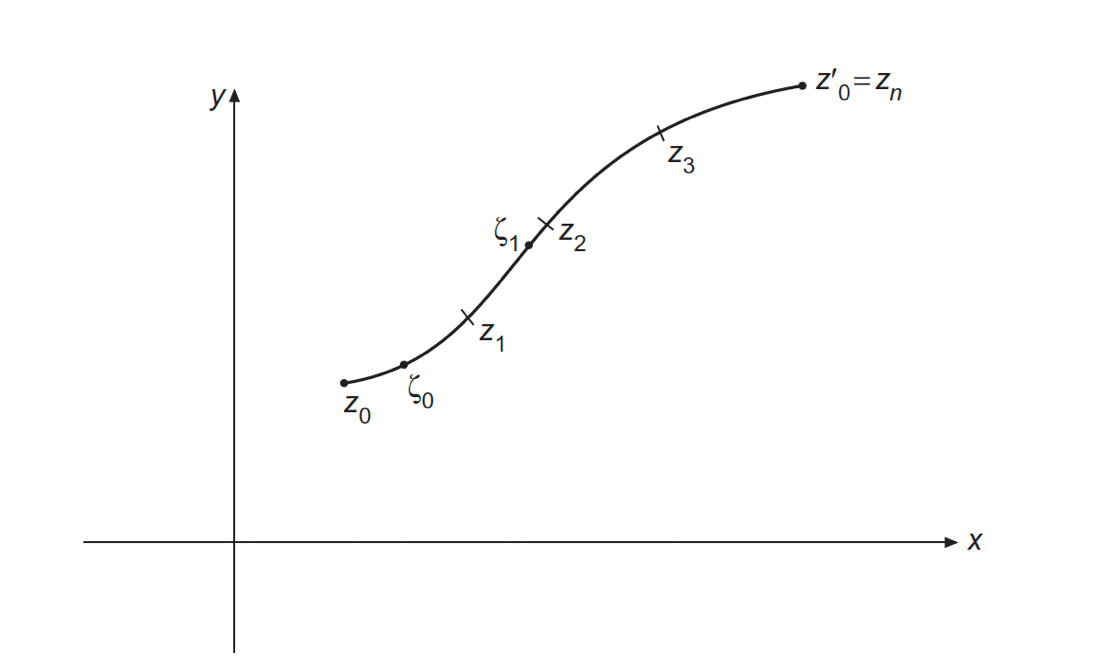
\includegraphics[width=0.5\linewidth]{fig13.png}
\end{figure}

\noindent
Integrals in the complex plane are defined in a way analogous to those in two dimensions
\begin{itemize}
    \item define a path of integration
    \item divide the path in $n$ steps and approximate the integral with a sum
\[
S_n = \sum_{j=1}^{n} f(\zeta_j)(z_j - z_{j-1})
\]
    \item take the limit for $n\rightarrow \infty$ (if it exists!)
\end{itemize}
\begin{equation}
    \lim_{n \to \infty} \sum_{j=1}^{n} f(z_j)(z_j - z_{j-1})
= \int_{z_0}^{z_0'} f(z) \, dz
= \int_{C} f(z) \, dz
\end{equation}
Explicitly:
\begin{equation}
    \int_{z_1}^{z_2} f(z) \, dz
= \int_{(x_1, y_1)}^{(x_2, y_2)} (u + iv)(dx + i dy)
= \int_{(x_1, y_1)}^{(x_2, y_2)} (u\, dx - v\, dy) + i \int_{(x_1, y_1)}^{(x_2, y_2)} (u\, dy + v\, dx)
\end{equation}
It means sum of real integrals in 2-dim plane.

\vspace{2mm} \noindent
\textbf{Integral along a closed path (Cauchy’s theorem)}
Let’s take a function analytic in a simply connected region $A$ of the complex plane and with $C$ its closed contour and calculate the integral along $C$
\begin{figure}[h]
    \centering
    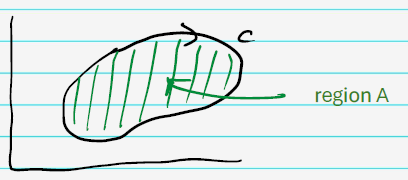
\includegraphics[width=0.3\linewidth]{fig14.png}
\end{figure}

\newpage
\begin{equation}
    \oint_{C} f(z) \, dz
= \oint_{C} \left[ u(x, y) \, dx - v(x, y) \, dy \right]
+ i \oint_{C} \left[ v(x, y) \, dx + u(x, y) \, dy \right]
\end{equation}
The two real integrals in the $$(x,y)$$ plane are the circuitations of two vector fields:
\begin{equation}
    \vec{V}(x, y) = \begin{bmatrix} u(x, y),\ -v(x, y) \end{bmatrix}, \quad
\vec{W}(x, y) = \begin{bmatrix} v(x, y),\ u(x, y) \end{bmatrix} \, \quad \text{when $d\vec{r} = (dx, dy)$}
\end{equation}
Then:
\begin{equation}
    \oint_C f(z)\,dz 
= \oint_C \vec{V} \cdot d\vec{r} 
+ i \oint_C \vec{W} \cdot d\vec{r}
\end{equation}
Can calculate the two integrals using Stokes theorem:
\begin{equation}
    \oint_C f(z) \, dz
= \iint_A \left( \frac{\partial V_y}{\partial x} - \frac{\partial V_x}{\partial y} \right) dx\,dy
+ i \iint_A \left( \frac{\partial W_y}{\partial x} - \frac{\partial W_x}{\partial y} \right) dx\,dy
\end{equation}
Substituting the components of $V$ and $W$:
\begin{equation}
    \oint_C f(z) \, dz =
\iint_A \left( \cancel{-\frac{\partial v}{\partial x} - \frac{\partial u}{\partial y}} \right) dx\,dy
+ i \iint_A \left( \cancel{\frac{\partial u}{\partial x} - \frac{\partial v}{\partial y}} \right) dx\,dy
\end{equation}
Due to Cauchy-Riemann conditions both $V$ and $W$ are irrotational!

\vspace{3mm} \noindent
\textbf{Cauchy’s integral theorem}
\begin{theorem}[Cauchy’s integral theorem]
    If $f(z)$ is an analytic function at all points of a simply connected region in the complex plane and if $C$ is a closed contour within that region, then
    \begin{equation}
        \oint_C f(z)dz = 0
    \end{equation}
\end{theorem}

\noindent
\textbf{N.B.} A region is simply connected if every closed curve within it can be shrunk continuously to a point that is within the region. Simply said, it has no holes, otherwise Stoke’s theorem is not valid (the curls of $V$ and $W$ cannot be integrated in the full region).

\noindent
Cauchy’s theorem is equivalent to saying that the integral does not depend on the path of integration, but only on the initial and final points, provided that the different paths are within the analycity region (i.e., can deform the path of integration without changing the result if the deformation never crosses a singularity)
\begin{figure}[h]
    \centering
    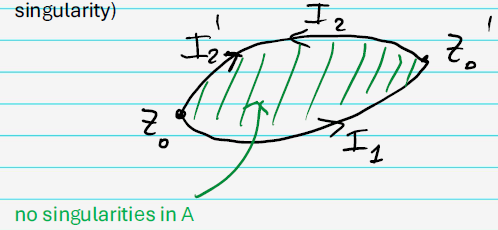
\includegraphics[width=0.5\linewidth]{fig15.png}
\end{figure}
\[
\oint f(z)\,dz = I_1 + I_2 \Rightarrow I_1 = -I_2
\]
\[
I_2' = -I_2 \Rightarrow I_1 = I_2'
\]

\newpage

\noindent
This is exactly what we need to apply to complex integrals the same rules of real integrals!

\noindent
\textbf{For example:}
\begin{equation}
    \int_{z_0}^{z_1} z^3 \, dz 
= \left[ \frac{z^4}{4} \right]_{z_0}^{z_1}
= \frac{1}{4} \left( z_1^4 - z_0^4 \right)
\end{equation}
the result depends only on the initial and final points, but not on the path joining them.
\begin{figure}[h]
    \centering
    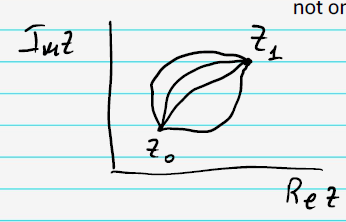
\includegraphics[width=0.3\linewidth]{fig16.png}
\end{figure}

\vspace{2mm}\noindent
\textbf{Cauchy’s integral formula}

\noindent
If the path contains a singularity Cauchy’s theorem is not valid. Let’s consider the integral:
\begin{equation}
    \oint_C \frac{f(z)}{z-z_0}dz
\end{equation}
on a closed path $C$ that is the boundary of a region $A$ that contains the point $z_0$, and where the function $f(z)$ is analytic. So:
\begin{equation}
    \lim_{z \rightarrow z_0} f(z) = f(z_0) \quad \color{blue}\text{``Well behaved''} \color{black}
\end{equation}
However, the $1/(z-z_0)$ factor is singular and if $z_0 \in A$ the integral does not obey Cauchy’s theorem. Nevertheless, we can always deform the path $C$ around $z_0$ if we do not cross other singularities to make it a circle $C(R)$ of radius $R$ without changing the result. Moreover, the result will not change taking the limit for $R \rightarrow 0$.
\begin{figure}[h]
    \centering
    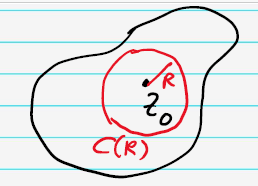
\includegraphics[width=0.3\linewidth]{fig17.png}
\end{figure}

\noindent
on the circle $C(R)$: $z-z_0 = Re^{i\varphi}$ and $dz = Re^{i \varphi} id\varphi$
\begin{align}
    \oint_{C(R)} \frac{f(z)}{(z - z_0)^n} \, dz
&= \lim_{R \to 0} \int_{0}^{2\pi}
\frac{f(z_0 + R e^{i\varphi}) R e^{i\varphi} \, i \, d\varphi}{R e^{i\varphi}}\\
&= \lim_{R \to 0} \int_{0}^{2\pi} i \, d\varphi \, f(z_0 + R e^{i\varphi})
= 2\pi i \, f(z_0)
\end{align}
For a real function, the existence of the $n$-th derivative does not guarantee that the $(n+1)$ the derivative exists. On the other hand, if a complex function $f(z)$ is differentiable, them it has all derivatives!

\noindent
they can be calculated using Cauchy’s integral formula:
\begin{align*}
    &f(z) = \frac{1}{2\pi i} \oint \frac{f(z')}{z' - z} \, dz' \quad  \frac{d f(z)}{d z} = \frac{1}{2\pi i} \oint \frac{f(z')}{(z' - z)^2} \, dz'\\
    &\frac{d^2 f(z)}{d z^2} = \frac{2}{2\pi i} \oint \frac{f(z')}{(z' - z)^3} \, dz' \quad \frac{d^n f(z)}{d z^n} = \frac{n!}{2\pi i} \oint \frac{f(z')}{(z' - z)^{n+1}} \, dz'
\end{align*}
exchange differentiation and integration
\newpage

\noindent
\textbf{Cauchy’s integral formula allows to prove Liouville’s theorem:}

\begin{center}
    \fbox{\color{red}If $f(z)$ is analytic and bounded in the entire complex plane it is a constant.\color{black}}
\end{center}

\noindent
write $f$ as a power expansion:
\begin{equation}
    f(z) = \sum_{n=0}^\infty a_n z^n
\end{equation}
then $|f(z)|<M$ on a circle of radius $r$ about the origin. In this case:
\begin{equation}
    a_n = \frac{1}{n!} \left. \frac{d^n f(z)}{d z^n} \right|_{z = 0}
= \frac{1}{2\pi i} \int_{|z| = r} \frac{f(z)}{z^{n+1}} \, dz
\end{equation}
and:
\begin{equation}
    |a_m| = \frac{1}{2\pi} \left|  \oint_{|z| = r} \frac{f(z)}{z^{m+1}} \, dz \right|
\leq \frac{M(r)}{2\pi} \cdot \frac{2\pi r}{r^{m+1}}  \  \ \Rightarrow \ \ 
|a_m| \leq \frac{M(r)}{r^m} \quad \color{red} \text{(Cauchy's inequality)} \color{black}
\end{equation}
then if $|f(z)|<M$ for all $z$ Cauchy’s inequality applied for $|z|=r$ gives:
\begin{equation}
    |a_n| < Mr^{-n}
\end{equation}
taking the limit $r \rightarrow \infty$ all the an go to zero with the exception of $a_0$. Then:
\begin{equation}
    f(z) = a_0  \quad \text{is a constant (Liouville’s theorem)}
\end{equation}

\begin{theorem}[Liouville's theorem]
    If $f(z)$ is analytic and bounded in the entire complex plane it is a constant.
\end{theorem}

\noindent
Liouville's theorem provides a straightforward proof of the Fundamental theorem of algebra.

\begin{theorem} [Fundamental theorem of algebra]
    Any polynomial $P(z) = \sum_{k=0}^n a_n z^n$ with $n>0$ and $a_n \neq 0$ has $n$ roots.
\end{theorem}

\noindent
Suppose $P(z)$ has no zeros. Then $1/P(z)$ is analytic and bounded in all the complex plane, including $|z| \to \infty$.
Then, according to Liouville's theorem, it should be a constant, which is not true.
Then we have to admit that $P(z)$ has at least one root $z_1$, and repeat the argument with the new polynomial $P_1 = P / (z - z_1)$.

\noindent
Also in this case, $P_1$ should be a constant, so we go on dividing by $(z - z_k)$ until $k = n$.
When we divide $P$ by exactly $n$ factors $(z - z_k)$, the polynomial $P_n$ reduces to degree zero and $1 / P_n$ is a constant,
in agreement with Liouville's theorem. As a consequence, $P(z)$ has exactly $n$ zeros.

\vspace{3mm} \noindent
\textbf{Taylor expansion}

\noindent
Suppose we want to expand the function $f(z)$ around the point $z=z_0$. Let’s express $f(z)$ using Cauchy’s integral formula on a radius $C(R)$ centered at $z=z_0$. $R$ must be less than the distance between $z_0$ and $z_1$, with $z_1$ the nearest singularity to $z_0$. In this way $f(z)$ is analytic on $C$.

\begin{figure}[h]
    \centering
    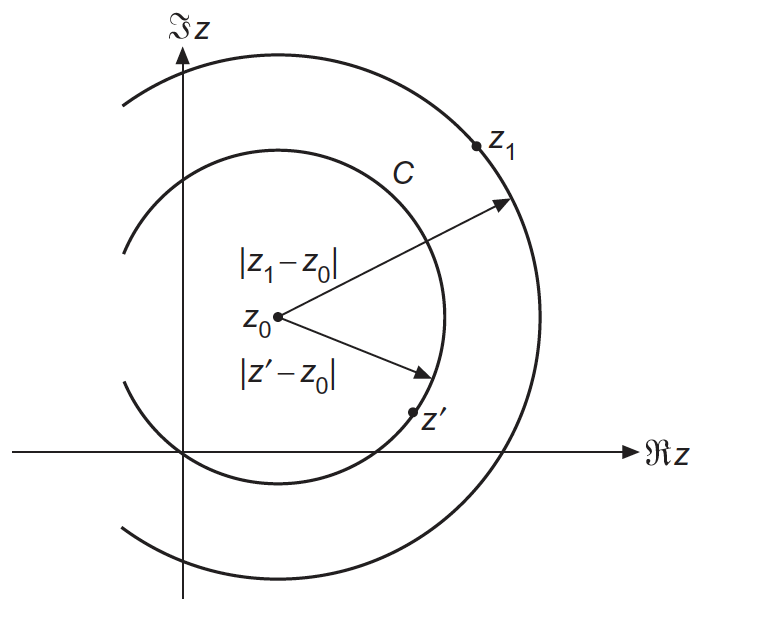
\includegraphics[width=0.35\linewidth]{fig18.png}
\end{figure}

\newpage
\begin{equation}
    f(z) = \frac{1}{2\pi i} \oint_C \frac{f(z')}{z' - z} \, dz'
\end{equation}
factor out a $1/(z’-z_0)$ term and express the rest using Cauchy’s integral formula for the derivatives
\begin{equation}
    f(z) = \frac{1}{2\pi i} \oint_C \frac{f(z')}{(z' - z_0) - (z - z_0)} \, dz' = \frac{1}{2\pi i} \oint_C \frac{f(z')}{(z' - z_0) \left(1 - \frac{z - z_0}{z' - z_0} \right)} \, dz'
\end{equation}
now use the identity:
\begin{equation}
    \frac{1}{1 - t} = 1 + t + t^2 + t^3 + \cdots
\end{equation}
that converges for $|t|<1$. In particular, for a point inside $C$:
\begin{equation}
    t = \frac{z - z_0}{z' - z_0}, \qquad |t| < 1
\end{equation}
so:
\begin{align}
    f(z) &= \frac{1}{2\pi i} \oint_C \frac{f(z')}{z' - z_0} 
\left[
1 + \frac{z - z_0}{z' - z_0}
+ \left(\frac{z - z_0}{z' - z_0}\right)^2
+ \left(\frac{z - z_0}{z' - z_0}\right)^3 + \cdots
\right] dz'\\
&= \frac{1}{2\pi i} \oint_C \sum_{n=0}^{\infty}
\frac{(z - z_0)^n f(z')}{(z' - z_0)^{n+1}} \, dz'
= \sum_{n=0}^{\infty} \frac{(z - z_0)^n}{2\pi i}
\oint_C \frac{f(z')}{(z' - z_0)^{n+1}} \, dz'
\end{align}
and using Cauchy integral formula for the derivatives:
\begin{equation}
    f(z) = \sum_{n=0}^{\infty} \frac{1}{n!} \left. \frac{d^n f}{dz^n} \right|_{z = z_0} (z - z_0)^n
\end{equation}
which is the Taylor expansion. The derivation shows that the expansion converges when:
\begin{equation}
    |z-z_0| < \underbrace{|z_1 - z_0|}_{\text{rad of conv.}}
\end{equation}
The Taylor series of a function $f(z)$ about any interior point $z_0$ of a region in which $f(z)$ is analytic is a unique expansion that will have a radius of convergence equal to the distance from $z_0$ to the singularity of f(z) closest to $z_0$, meaning that the Taylor series will converge within this circle of convergence. The Taylor series may or may not converge at individual points on the circle of convergence.

\vspace{3mm}\noindent
\textbf{Laurent expansion}

\noindent
Consider the function:
\begin{equation}
    f(z) = \frac{1}{z(z-1)} = \frac{1 - z + z}{z(z-1)} 
= \frac{1 - z}{z(z - 1)} + \frac{z}{z(z - 1)} 
= -\frac{1}{z} - \frac{1}{1 - z}
\end{equation}
the function is defined for $0<|z|<1$. Then:
\begin{equation}
    f(z) = -\frac{1}{z} - \sum_{n=0}^{\infty} z^n 
= -\frac{1}{z} - 1 - z - z^2 - z^3 
= -\sum_{n=-1}^{\infty} z^n = \sum_{n=-1}^{\infty} a_n z^n
\end{equation}
In Laurent series, $n$ can be negative.
\begin{equation}
    a_n =
\begin{cases}
-1 & \text{for } n \geq -1, \\
0 & \text{for } n < -1.
\end{cases}
\end{equation}

\newpage

\begin{figure}[h]
    \centering
    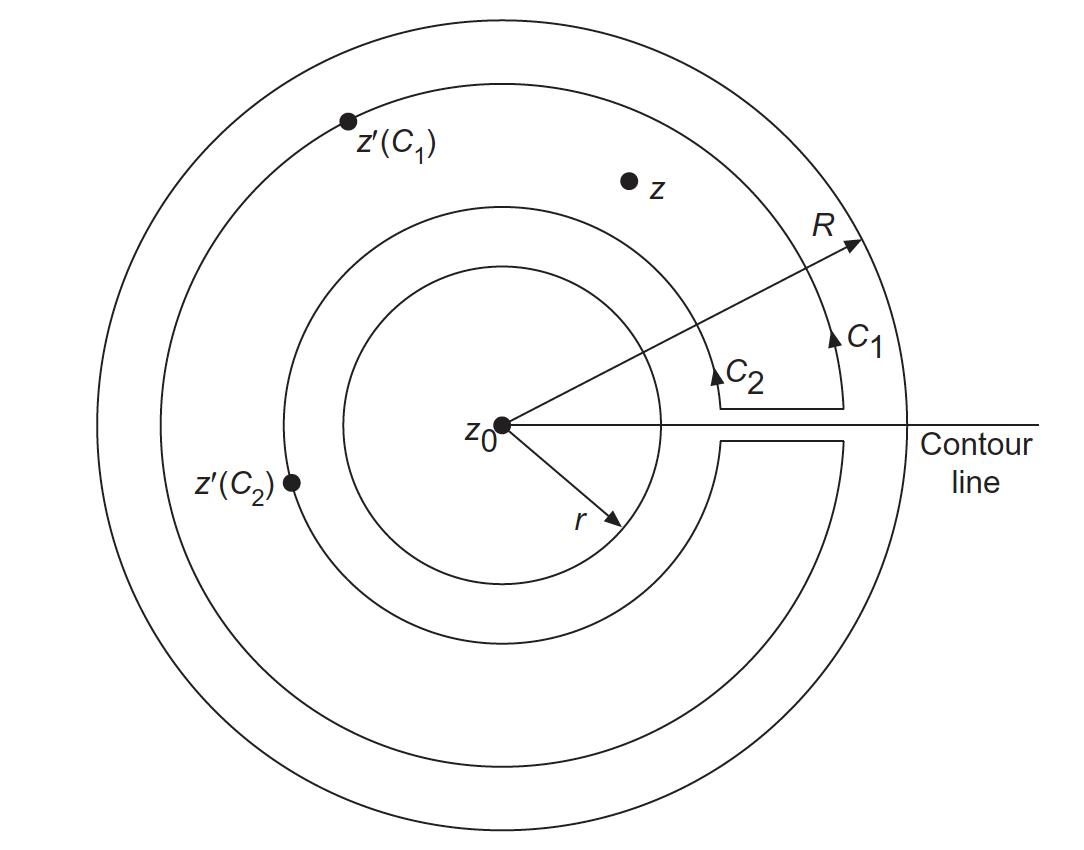
\includegraphics[width=0.5\linewidth]{fig19.png}
\end{figure}

\noindent
A Laurent series emerges when the function $f(z)$ is analytic on an annular region between circles of radius $r$ and $R$. Can convert the region in a simply connected one (i.e. with a single boundary) by drawing a barrier of infinitesimal thickness In this way the path $C$ (in red color) is simply connected. For $z$ inside it. Then:
\begin{equation}
    f(z) = \frac{1}{2\pi i} \oint_{C_1} \frac{f(z')}{z' - z} \, dz'
- \frac{1}{2\pi i} \oint_{C_2} \frac{f(z')}{z' - z} \, dz'
\end{equation}
\textbf{N.B.} $C_1$ is counterclockwise (positive), $C_2$ is clockwise (negative), and the contributions from $C_3$ and $C_4$ cancel. Now proceed as before writing both denominators as $(z’-z_0)-(z-z_0)$:
\begin{equation}
    f(z) = \frac{1}{2\pi i} \sum_{n=0}^{\infty} (z - z_0)^n 
\oint_{C_1} \frac{f(z')}{(z' - z_0)^{n+1}} \, dz' + S_2
\end{equation}
In the case of $S_2$ on the path $C_2$ we have $|z’-z_0|<|z-z_0|$ so:
\begin{align}
    S_2 &= -\frac{1}{2\pi i} \oint_{C_2} \frac{f(z')}{(z'-z_0) - (z-z_0)} \, dz'
= \frac{1}{2\pi i} \oint_{C_2} \frac{f(z')}{z'-z_0} 
\left[ \frac{1}{1 - \frac{z - z_0}{z' - z_0}} \right] dz'\\
&= \frac{1}{2\pi i} \oint_{C_2} \frac{f(z')}{z'-z_0} 
\sum_{n=0}^{\infty} \left( \frac{z - z_0}{z' - z_0} \right)^n dz'
= \frac{1}{2\pi i} \sum_{n < 0} (z - z_0)^n 
\oint_{C_2} \frac{f(z')}{(z' - z_0)^{n+1}} dz'\\
&= \frac{1}{2\pi i} \sum_{n=1}^{\infty} (z - z_0)^{-n} 
\oint_{C_2} (z' - z_0)^{n-1} f(z') \, dz'
\end{align}
So:
\begin{equation}
    f(z) = S_1 + S_2 \quad \text{$S_1$ converges inside $S_1$ while $S_2$ converges outside $S_2$}
\end{equation}
Combining the two terms we obtain the series:
\begin{equation}
    f(z) = \sum_{n=-\infty}^{+\infty} a_n (z - z_0)^n \quad \text{with} \quad a_n = \frac{1}{2\pi i} \oint_C \frac{f(z')}{(z' - z_0)^{n+1}}\, dz'
\end{equation}
$C$ can be any contour within the annular region that encircles $z_0$ in a counterclockwise sense.

\noindent
\textbf{N.B.} Laurent series contains negative powers of $(z-z_0)$.

\noindent
Going back to the function:
\begin{equation}
    f(z) = \frac{1}{z(z-1)}
\end{equation}
It is defined in an annular region because it diverges for $|z|=0$ and $|z|=1$. It's Laurent expansion around the origin is:
\begin{equation}
    f(z) = \sum_{n=-\infty}^{\infty} a_n z^n
\end{equation}

\newpage
\begin{equation}
    a_n = \frac{1}{2\pi i} \oint_C \frac{f(z')}{(z')^{n+1}} \, dz'
= \frac{1}{2\pi i} \oint_C \frac{1}{(z')^{n+2}(z'-1)} \, dz'
= -\frac{1}{2\pi i} \oint_C \sum_{k=0}^{\infty} (z')^{k - n - 2} \, dz'
\end{equation}
Using:
\begin{equation}
    \frac{1}{1-z'} = \sum_m (z')^m \qquad z' = r e^{i\varphi}, \qquad dz' = r e^{i\varphi} i\, d\varphi
\end{equation}
Then:
\begin{align}
    I =& \frac{1}{2\pi i} \oint z'^{ \ m - n - 1} \, dz' = \frac{1}{2\pi i} \int_0^{2\pi} r e^{i\varphi} \, i \, d\varphi \cdot r^{m - n - 1} e^{i(m - n - 1)\varphi} \\
=& \frac{1}{2\pi} \int_0^{2\pi} r^{m - n} e^{i(m - n)\varphi} \, d\varphi
\end{align}
Unless $m=n$ the integrand is periodic in the interval $0<\varphi<2\pi$ and the integral vanishes. For $m=n$:
\begin{equation}
    I = \frac{1}{2\pi} \int_0^{2\pi} d \varphi = 1
\end{equation}
So:
\begin{equation}
    I = \delta_{nm} = 
\begin{cases}
1 & \text{for } n = m \\
0 & \text{otherwise}
\end{cases}
\end{equation}
\begin{align}
    a_n &= \frac{1}{2\pi i} \oint_C \frac{f(z')\,dz'}{(z')^{n+1}} 
= -\frac{1}{2\pi i} \oint_C \sum_{m=0}^{\infty} (z')^{m - n - 2} \, dz'\\
&= -\sum_{m=0}^{\infty} \delta_{m, n+1}
= \begin{cases}
-1 & \text{if } n \geq -1 \\
0 & \text{if } n < -1
\end{cases}
\end{align}

\section{Handout 05}

\noindent
\textbf{Poles}

\noindent
Let’s consider an isolated singular point $z_0$, i.e. a point where the function $f(z)$ is not analytic, but is analytic at neighboring points. It is then possible to calculate a Laurent expansion around $z_0$.
\begin{itemize}
    \item If the most negative power of the expansion is a finite number $n$ the singularity is a \textbf{pole of order} $n$ ($n=1$ is also referred to as a simple pole)
    \item If the Laurent expansion continues to negative infinite powers the pole has infinite order and is called an \textbf{essential singularity}
\end{itemize}

\noindent
In alternative, the order of the pole is the smallest integer $n$ for which the limit:

\begin{equation}
    \lim_{z \rightarrow z_0} (z-z_0)^n f(z) \quad \text{ exists}
\end{equation}
\begin{itemize}
    \item A function that is analytic everywhere except for isolated poles is called \textbf{meromorphic}
    \item A function with no singularities in the finite complex plane is \textbf{entire}
    \item A function that has no singularities including infinity is \textbf{constant} (Liouville theorem)
\end{itemize}

\newpage

\noindent
\textbf{Branch points}

\noindent
Singularities associated to multi-values functions. Consider the function $f(z) = z^{1/2}$ setting: (when $k \in \mathbb{Z}$
\begin{equation}
    z = r e^{i(\varphi + 2k\pi)}
\quad \Rightarrow \quad f(z) = r^{1/2} e^{i\frac{\varphi}{2} + i k\pi}
\end{equation}
We can choose a specific value of $k$ (for instance, $k=0$) and move along a circular path in such a way that the function is continuous. (i.e., we keep the same value of $k$) However, after a complete revolution on a closed path around the origin the function does not return to the same value:
 \begin{figure}[h]
     \centering
     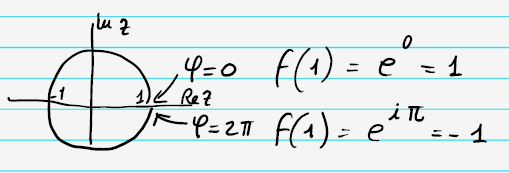
\includegraphics[width=0.5\linewidth]{fig20.png}
 \end{figure}

\noindent
After a second revolution the function eventually returns to its original value:
\begin{equation}
    f\left(e^{i 4\pi}\right) = \left(e^{i 4\pi}\right)^{1/2} = e^{i 2\pi} = 1
\end{equation}
We say that the function $f(z)=z^{1/2}$ has a branch point in $z=0$ with order 2.

\noindent
\textbf{Order}: minimal number of revolution required to return to the starting value of the function

\noindent
\textbf{N.B.} Note that if instead we calculate the function along a path that does not contain the origin after a complete path it returns to the original value:

\begin{figure}[h]
    \centering
    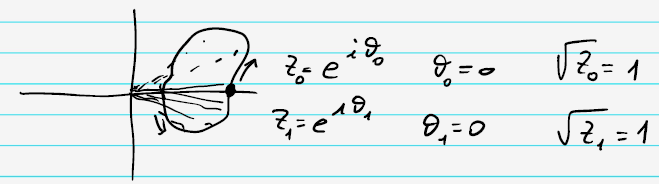
\includegraphics[width=0.5\linewidth]{fig21.png}
\end{figure}

\noindent
In other words, the function does not return to the original value only when the path encircles the branch point. A multivalued function can be restricted to single-valuedness on a portion of the complex plane by imposing a prescription that prevents to encircle a branch point.

\noindent
Branch cut:
\begin{figure}[h]
    \centering
    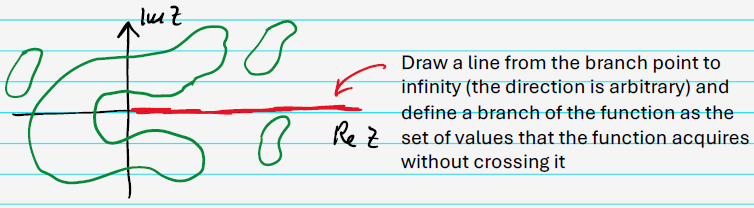
\includegraphics[width=0.7\linewidth]{fig22.png}
\end{figure}

\noindent
Each branch of a multi-valued function $f(z)$ is now single-valued. In each branch one has:
\begin{equation}
    z = re^{i \varphi + i 2n\pi}
\end{equation}
with fixed $n$. So $n=0$ is a branch (sometimes called principal branch) where in each point $f(z)$ acquires its principal value. $n=1$ is another branch, and so on.

\noindent
\textbf{N.B. }Across the branch $f(z)$ is discontinuous. However, within each branch Cauchy’s theorem is valid.

\newpage

\noindent
\textbf{Infinite number of branches}

\noindent
take the logarithm function:
\begin{equation}
    \ln z = \ln\left(r e^{i(\varphi + 2n\pi)}\right) = \ln r + i(\varphi + 2n\pi)
\end{equation}
in this case the order of the branch at $z=0$ is infinite.

\noindent
Power of $z$:
\begin{equation}
    f(z) = z^{\alpha} = e^{\alpha \ln z} = e^{\alpha [\ln r + i (\varphi + 2n\pi)]} = e^{\alpha \ln r} \cdot e^{i \alpha \varphi + i \alpha 2n\pi}
\end{equation}
If $\alpha$ = integer the function is single valued. If $\alpha = k/m$ (with $k,m$ integers) is a rational number:
\begin{equation}
    \alpha n = \frac{k}{m} n \quad \Rightarrow \text{for }n=m, \ \ \alpha n = k \quad \Rightarrow \quad \color{red} \text{$m$-valued function} \color{black}
\end{equation}
If $\alpha$ is real the function has infinite values.

\vspace{3mm} \noindent
\textbf{Multiple branch points}

\noindent
Consider the function:
\begin{equation}
    f(z) = \sqrt{z^2 - 1} = (z+1)^{1/2} (z-1)^{1/2}
\end{equation}
which has two branch points, one at $z_1 =1$ and the other at $z_2 =-1$. One way to make it single-values is to draw a branch cut from $z_1$ to $z_2$. Another way is to draw two branch cuts, one from $z_1$ to $-\infty$, the other from $z_2$ to $+\infty$:
\begin{figure}[h]
    \centering
    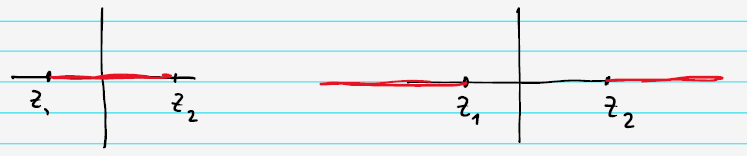
\includegraphics[width=0.75\linewidth]{fig23.png}
\end{figure}

\noindent
in both ways (there are infinite more) the branch of $f(z)$ is single-valued, because neither $z_1$ nor $z_2$ is encircled. Suppose we want to evaluate $f(z)$ along the path $C$ shown in the plot.

\begin{figure}[h]
    \centering
    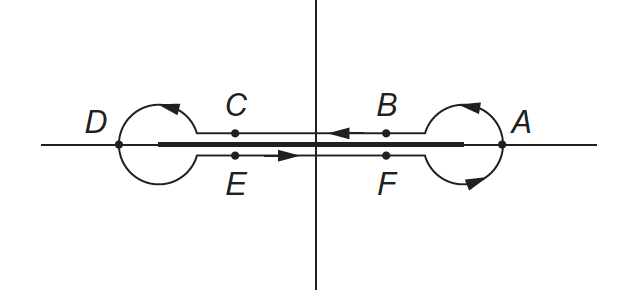
\includegraphics[width=0.35\linewidth]{fig24.png}
\end{figure}

\noindent
Across the cut the function is discontinuous. So even if the path $C$ is infinitely close to the $\Re (z)$ axis both above and below it the value of the phase will be different:

\begin{figure}[h]
    \centering
    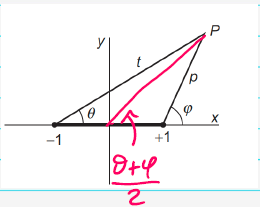
\includegraphics[width=0.35\linewidth]{fig25.png}
\end{figure}

\newpage

\noindent
We evaluate the phase with respect to the origin, so the phase of the argument is $(\theta + \psi)/2$.

\begin{figure}[h]
    \centering
    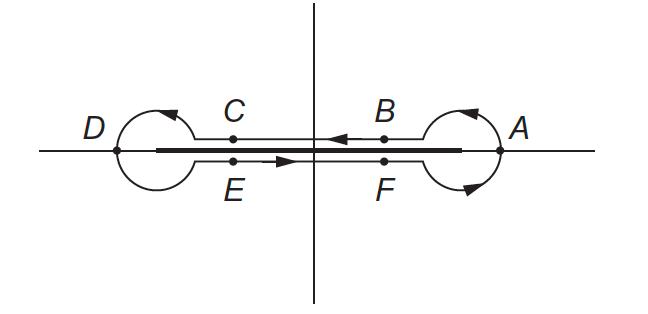
\includegraphics[width=0.4\linewidth]{fig26.png}
\end{figure}

\begin{figure}[h]
    \centering
    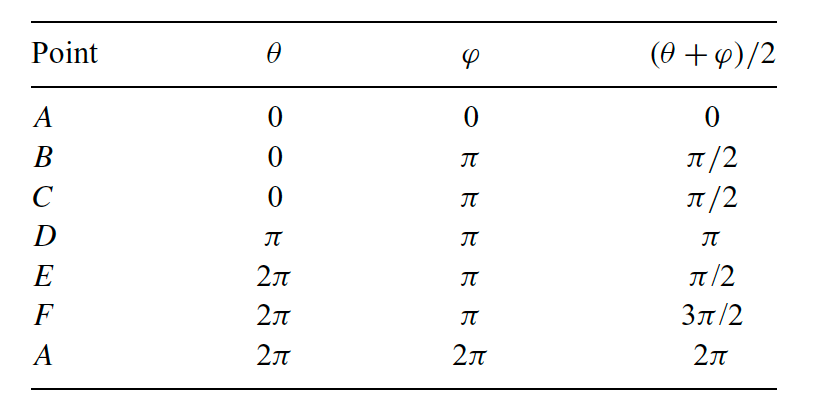
\includegraphics[width=0.5\linewidth]{fig27.png}
\end{figure}

\begin{itemize}
    \item In $B$ and $C$ (above the cut) the phase sis different than in $E$ and $F$ (below the cut)
    \item After a full revolution returns to original value
\end{itemize}

\noindent
\textbf{Analytic continuation}

\noindent
An analytic function can be uniquely expanded in a Taylor series about an interior point $z_0$ of its region of analyticity. If there is a singularity $z_s$ the radius of convergence will be the distance from $z_0$ and $z_s$ that will define a circle of convergence $A_1$.

\begin{figure}[h]
    \centering
    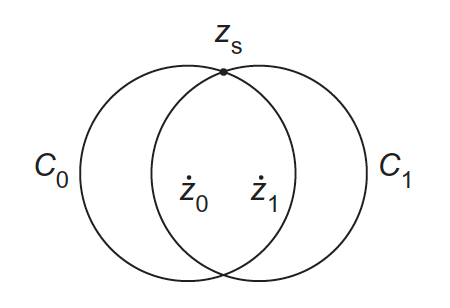
\includegraphics[width=0.4\linewidth]{fig28.png}
\end{figure}

\noindent
To extend the region of analyticity of $f(z)$, one can make an expansion around another point $z_1$ that will have another region of analyticity $A_2$. In the overlap between $A_1$ and $A_2$, the two expansions will yield same values.

\vspace{2mm}\noindent
In particular, the coefficients in the Taylor series are proportional to the derivatives of $f(z)$. An analytic function has derivatives of all orders that are independent of direction, and so the values of $f(z)$ on a single finite line segment with $z_0$ as an interior point will suffice to determine all derivatives of $f(z)$ at $z = z_0$.

\vspace{2mm}\noindent
If two analytic functions have values that coincide on a continuous range (as small as a segment), they are the same function \underline{\textbf{everywhere}}!

\newpage

\noindent
If there is only a singular point it is then possible to define the function all around it joining different Taylor expansions.

\begin{figure}[h]
    \centering
    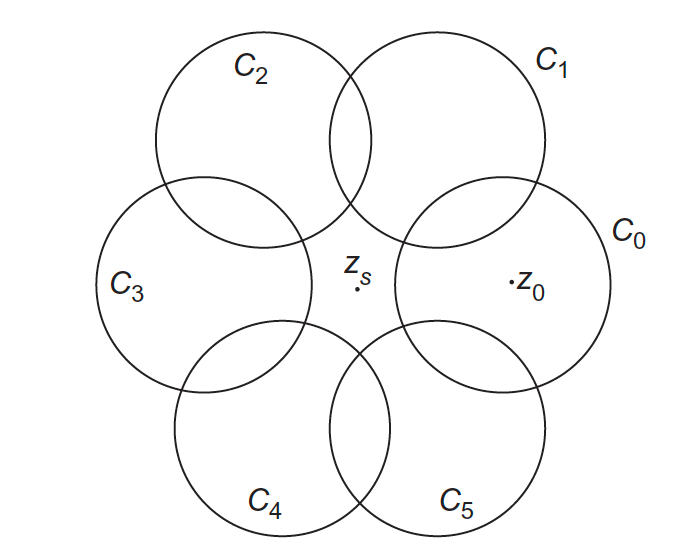
\includegraphics[width=0.4\linewidth]{fig29.png}
\end{figure}

\noindent
\textbf{Residue Theorem}

\noindent
If the Laurent expansion of a function:
\begin{equation}
    f(z) = \sum_{n = -\infty}^{+\infty} a_n (z-z_0)^n
\end{equation}
is integrated term by term on a closed contour that encircles a singular point $z_0$ (once, counterclockwise) then:
\begin{equation}
    a_n \int (z-z_0)^n dz = 0 \quad (n \neq -1)
\end{equation}
for $n=-1$:
\begin{equation}
    a_{-1} \int (z-z_0)^{-1} dz = 2\pi i a _{-1}
\end{equation}
So:
\begin{equation}
    \oint f(z)dz = 2\pi i a_{-1}
\end{equation}
Only the $n=-1$ term contributes to the integral. \color{red} The constant $a_{-1}$ is called the \textbf{residue} of $f(z)$ at $z=z_0$. \color{black}

\noindent
Consider now a path that contains multiple isolated singularities:

\begin{figure}[h]
    \centering
    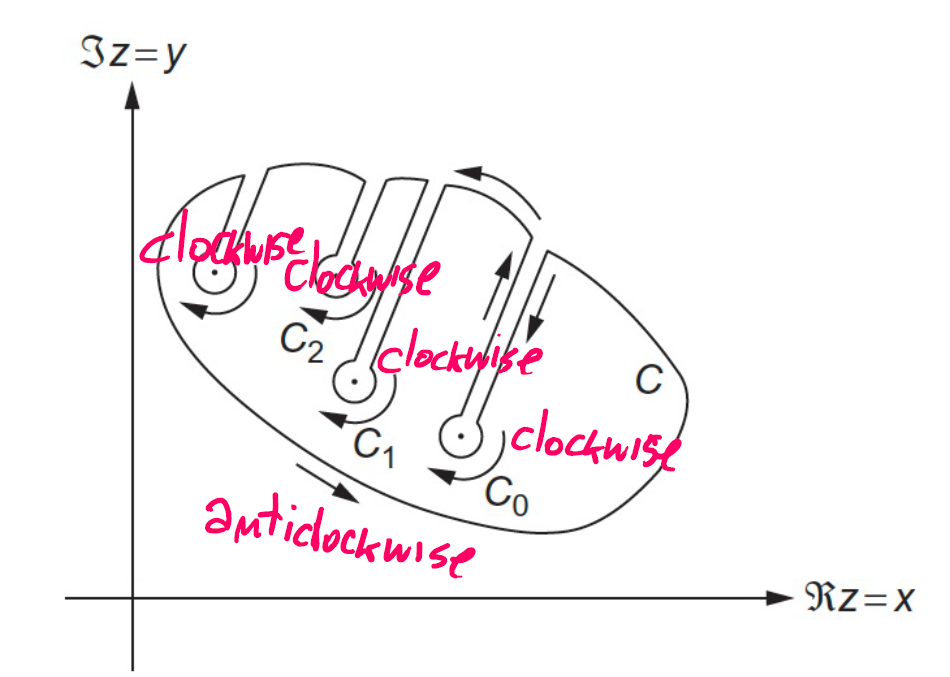
\includegraphics[width=0.5\linewidth]{fig30.png}
\end{figure}

\noindent
can deform the path encircling each of the singularities, obtaining:
\begin{equation}
    \oint_C f(z)\,dz + \oint_{C_1} f(z)\,dz + \oint_{C_2} f(z)\,dz + \cdots = 0
\end{equation}
$C$ is counterclockwise, but $C_1$, $C_2$, $\cdots$, $C_n$ are clockwise.

\newpage

\noindent
For each path $C_1$ the integral is:
\begin{equation}
    \oint_{C_i} f(z)\,dz = -2\pi i\, a_{-1,i}
\end{equation}
with $a_{-1,i}$ the residue obtained from the Laurent expansion around $z=z_i$ (negative sign because $C_i$ is clockwise). Then from:
\begin{equation}
    \oint_C f(z)\,dz + \oint_{C_1} f(z)\,dz + \oint_{C_2} f(z)\,dz + \cdots = 0 \quad \Rightarrow \quad  \oint_C f(z)\,dz = 2\pi i \left( a_{-1,1} + a_{-1,2} + \cdots \right)
\end{equation}
In other words:
\begin{equation}
    \boxed{\frac{1}{2\pi i} \oint_C f(z)\,dz = \text{(Sum of the residues inside $C$})} \quad \color{red} \text{(Residue Theorem)} \color{black}
\end{equation}

\noindent
\textbf{Explicit calculation of residues}

\noindent
Let's consider a function \( f(z) \) in the neighborhood of an isolated polar singularity \( z_0 \) of order \( n \). This means that the function \( f(z) \) can be written as:
\begin{equation}
    f(z) = \frac{g(z)}{(z - z_0)^n}
\end{equation}
with \( g(z) \) a function analytic in \( z_0 \), i.e., a function with Taylor expansion:
\begin{equation}
    g(z) = \sum_{k=0}^{\infty} \frac{1}{k!} \left. \frac{d^k g}{dz^k} \right|_{z = z_0} (z - z_0)^k = \sum_{k=0}^{\infty} g_k (z - z_0)^k
\end{equation}
The residue of \( f(z) \) is the term \( a_{-1} \) of the Laurent series of \( f(z) \):
\begin{equation}
    f(z) = \sum_{i=-n}^{\infty} a_i (z - z_0)^i 
= \frac{1}{(z - z_0)^n} \sum_{k=0}^{\infty} g_k (z - z_0)^k 
= \sum_{k=0}^{\infty} g_k (z - z_0)^{k - n}
\end{equation}
So in the sum we need to take only the coefficient \( g_k \) of the term proportional to \( (z - z_0)^{-1} \),  
i.e., we need \( k - n= -1 \Rightarrow k = n - 1 \):

\noindent
Residue:
\begin{equation}
    \left\{ \text{Res}(f(z)) \right\}_{z = z_0} 
= \frac{1}{2\pi i} \oint_C f(z)\,dz 
= g_{n-1} = 2\pi i \cdot \frac{1}{(n-1)!} \left. \frac{d^{n-1} g}{dz^{n-1}} \right|_{z = z_0}
\end{equation}
\begin{equation}
    = \frac{1}{(n-1)!} \lim_{z \to z_0} \left[ \frac{d^{n-1}}{dz^{n-1}} \left( f(z) (z - z_0)^n \right) \right]
\end{equation}


\vspace{3mm} \noindent
\textbf{Cauchy Principal Value}

\noindent
If an isolated pole is on the contour of an integration the integral diverges.

\begin{figure}[h]
    \centering
    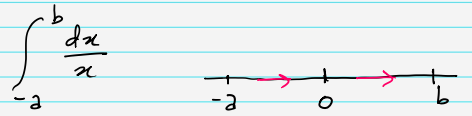
\includegraphics[width=0.5\linewidth]{fig31.png}
\end{figure}

\noindent
can remove the singularity from the path (change variable from $x$ to $–x$)
\begin{equation}
    \lim_{\delta \to 0^+} \left\{ \int_{-a}^{-\delta} \frac{dx}{x} + \int_{\delta}^{b} \frac{dx}{x} \right\} 
= \lim_{\delta \to 0^+} \left[ \int_{a}^{\delta} \frac{dx}{x} + \int_{\delta}^{b} \frac{dx}{x} \right] = \lim_{\delta \to 0^+} \left[ \cancel{\ln \delta} - \ln a + \ln b \cancel{- \ln \delta} \right] 
= \ln{\frac{b}{a}}
\end{equation}

\newpage

\noindent
Interestingly, the result of the limit is finite. However, this procedure does not make the result finite, because it depends on the way we approach the singularity. The limit we need to do is:
\begin{equation}
    \lim_{\delta_1, \, \delta_2 \to 0^+}
\left[
\int_{-a}^{-\delta_1} \frac{dx}{x}
+
\int_{\delta_2}^{b} \frac{dx}{x}
\right] \quad \text{with $\delta_1$ and $\delta_2$ independent}
\end{equation}
In the previous example, we assumed $\delta_1$=$\delta_2$ = $\delta$. However, suppose we adopt instead $\delta_1=2\delta_2$ (i.e. $\delta_1=2\delta$ and $\delta_2=\delta$). The result changes! 
\begin{equation}
    \lim_{\delta \to 0} 
\int_{-a}^{-2\delta} \frac{dx}{x}
+ 
\int_{-\delta}^{b} \frac{dx}{x}
=
\int_{a}^{2\delta} \frac{dx}{x}
+
\int_{-\delta}^{b} \frac{dx}{x}
=
\lim_{\delta \to 0}
\left[
\ln 2\delta - \ln 2 + \ln b - \ln \delta
\right]=
\ln \frac{b}{a} + \ln 2
\end{equation}
In other words, the integral is really divergent, and the limit has no definite value.

\noindent
Anyway, the limit assuming $\delta_1=\delta2= \delta$ is useful in the calculation of integrals, so it is defined as the Cauchy principal value.
\begin{equation}
    \lim_{\delta \to 0^+} \int^{x_0 - \delta} f(x)\, dx + \int_{x_0 + \delta} f(x)\, dx
\end{equation}
Cauchy principal value of the real integral of a function $f(x)$ with an isolated singularity on the integration path at the point $x_0$. Notation to indicate Cauchy’s principal value:
\begin{equation}
    P \int f(x)\, dx \quad \text{or} \quad \fint f(x)\, dx
\end{equation}
As we saw the Cauchy principal value will never be the integral that we are looking for. However, it can be one of the ingredients, provided that we complete the missing part (removed by the limiting procedure) in the complex plane.
\begin{figure}[h]
    \centering
    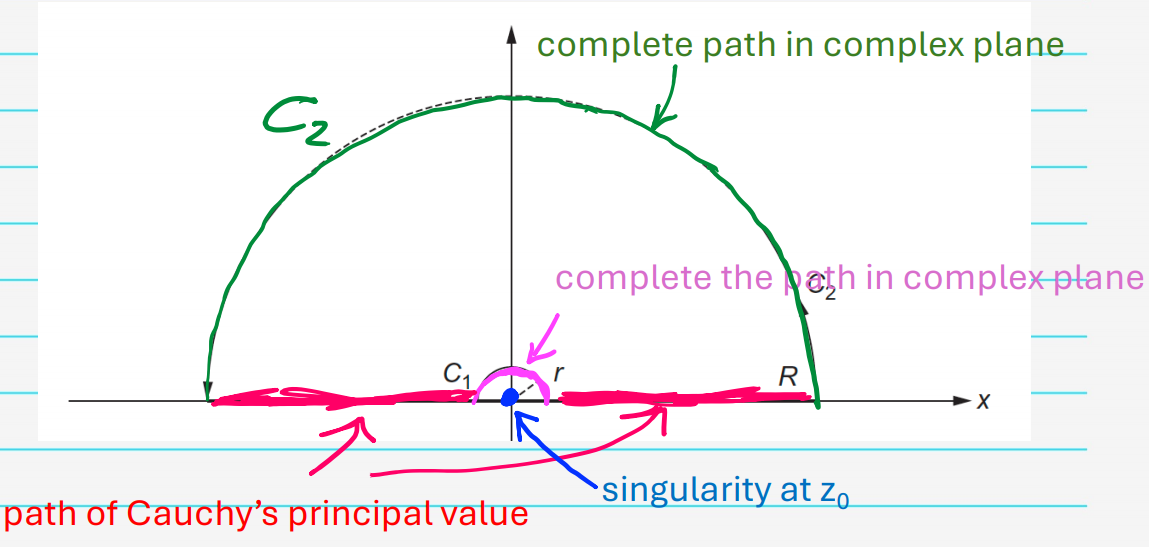
\includegraphics[width=0.6\linewidth]{fig32.png}
\end{figure}

\noindent
Can either pass above the singularity (as in the plot) or below. (small semicircle radius=$r$ large semicircle radius=$R$)

\noindent
Contour integral of the function $f(z)$ on the closed path shown above:
\begin{equation}
    \oint_C f(z)\,dz = \fint f(z)\,dz + I_{\text{over}} + \int_{C_2} f(z)\,dz = 2\pi i \sum (\text{residues except } z_0)
\end{equation}
\begin{equation}
    I_{\text{over}} \equiv \int_{C_1} f(z)\,dz
\end{equation}
With $I_{\text{over}}$ the integral over a small semicircle of radius $r$
\begin{figure}[h]
    \centering
    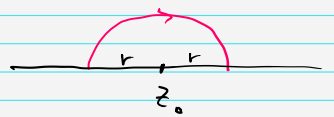
\includegraphics[width=0.35\linewidth]{fig33.png}
\end{figure}

\newpage
\noindent
Let’s assume that there is a simple pole in $z_0$. Then the function $f(z)$ has the Laurent expansion:
\begin{equation}
    f(z) = \sum_{n=-1}^{\infty} a_n (z - z_0)^n = \frac{a_{-1}}{z - z_0} + a_0 + a_1 (z - z_0) + \cdots
\end{equation}

\noindent
Let’s do the integral explicitly: when $z-z_9 = re^{i\theta}$ and $dz = ire^{i\theta} d\theta$
\begin{equation}
    I_{\text{over}} = \int_C f(z) dz = \int_\pi^0 ire^{i\theta} d\theta \left[ \frac{a_{-1}}{re^{i\theta}} + a_0 + a_1 re^{i\theta} + \cdots \right] \quad \textcolor{red}{\text{notice that the path is clockwise!}}
\end{equation}
Let's take $r = \delta$ and $\delta \rightarrow 0$
\begin{align*}
    I_{\text{over}} &= \lim_{\delta \rightarrow 0} \int_\pi^0 ire^{i\theta} d\theta \left[ \frac{a_{-1}}{re^{i\theta}} + a_0 + a_1 re^{i\theta} + \cdots \right] \\ & = \lim_{\delta \rightarrow 0} \int_\pi^0 (ia_{-1} + \cancel{i\delta e^{i\theta}a_0 } + \cdots) d\theta \quad \textcolor{red}{\text{vanishes, together with all the terms after it}}
\end{align*}
if instead, we had chosen to complete the path below the singularity:
\begin{figure}[h]
    \centering
    
\includegraphics[width=0.3\linewidth]{fig34.png}
\end{figure}
\begin{equation}
    I_{\text{under}} = \lim_{\delta \to 0} \int_{\pi}^{2\pi} d\theta\, i \delta e^{i\theta} 
\left[ \frac{a_{-1}}{\delta e^{i\theta}} + a_0 + \cdots \right] 
= \int_{\pi}^{2\pi} \left(i a_{-1} + i \delta e^{i\theta} a_0 + \cdots \right) d\theta 
= i \pi\, a_{-1}
\end{equation}
more on the use of Cauchy’s principal value later.

\vspace{2mm}\noindent
\textbf{Evaluation of definite integrals in the complex plane}

\noindent
Definite integrals of real functions can be calculated in the complex plane either by a change of variable or by extending the path of integration from the real axis to the complex plane
\begin{equation}
    I = \int_0^{2\pi} f(\sin\theta,\cos\theta)d\theta
\end{equation}
with $f$ a finite rational (i.e. single-valued) function for all values of $\theta$. Map $0<\theta<2\pi$ into the circle of radius $m_1$ in the complex plane:
\begin{figure}[h]
    \centering
    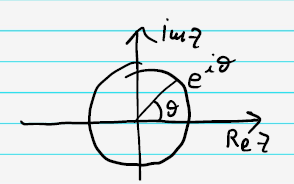
\includegraphics[width=0.3\linewidth]{fig35.png}
\end{figure}
$$z = e^{i\theta} \quad dz = ie^{i\theta} \quad \Rightarrow \quad d\theta = \frac{dz}{iz} = -i\frac{dz}{z}$$
and,
\begin{equation}
    \cos \theta = \frac{e^{i\theta} + e^{-i\theta}}{2} = \frac{z + z^{-1}}{2}, \quad
\sin \theta = \frac{e^{i\theta} - e^{-i\theta}}{2i} = \frac{z - z^{-1}}{2i}
\end{equation}
\textbf{N.B.} The original function f does not have any singularity, but the change of variable introduced a simple pole through $d\theta=-1dz/z$. So the integral over the circular path can be different from zero:
\begin{equation}
    I = -i \oint \left( \frac{z - z^{-1}}{2i} \cdot \frac{z + z^{-1}}{2} \right) \frac{dz}{z}
= -i \cdot 2\pi i \sum \text{(residues in the circle)}
\end{equation}
\textcolor{red}{\textbf{Powerful!}}

\newpage

\noindent
\textbf{Example \#1}
\begin{equation}
    I = \int_0^{2\pi} \frac{d\theta}{1 + a\cos\theta} \qquad |a| < 1
\end{equation}
change variable:
\begin{equation}
    I = -i \oint_C \frac{dz}{z \left[ 1 + \frac{a}{2}\left(z + \frac{1}{z} \right) \right]}
= -i \oint_C \frac{dz}{z + \frac{a}{2}z^2 + \frac{a}{2}}
= -\frac{2i}{a} \oint_C \frac{dz}{z^2 + \frac{2}{a}z + 1}
\end{equation}
zeros of denominator:
\begin{equation}
    az^2 + 2z + a = 0 \quad z = \frac{-1 \pm \sqrt{1-a^2}}{a}
\end{equation}
then:
\begin{equation}
    z_1 = -\frac{1 + \sqrt{1-a^2}}{a}, \quad z_2 = -\frac{1 - \sqrt{1-a^2}}{a}
\end{equation}
since $z_1 z_2 = 1$, the factor with larger absolute value $z_1$ has $|z_1|>1$ (outside unit circle) and the other has $|z_2|<1$ (inside unit circle):
\begin{figure}[h]
    \centering
    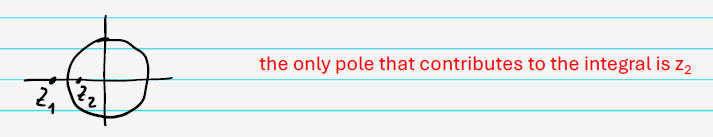
\includegraphics[width=0.75\linewidth]{fig36.png}
\end{figure}

\noindent
then:
\begin{align}
        I &= -\frac{2i}{a} \oint \frac{dz}{(z - z_1)(z - z_2)}
= -\frac{2i}{a} \cdot 2\pi i \cdot \operatorname{Res}\left( \frac{1}{(z - z_1)(z - z_2)}\right)_{z=z_2}\\
&= \frac{4\pi}{a} \lim_{z \to z_2} \frac{\cancel{(z - z_2)}}{(z - z_1)\cancel{(z - z_2)}}
= \frac{4\pi}{a(z_2 - z_1)}
\end{align}
substituting $z_1$ and $z_2$ in the result:
\begin{equation}
    I = \frac{4\pi}{a} \cdot \frac{1}{\frac{-1 - \sqrt{1 - a^2}}{2} + \frac{1 + \sqrt{1 - a^2}}{2}} 
= \frac{4\pi}{\cancel{1} + \sqrt{1 - a^2} \cancel{- 1} + \sqrt{1 - a^2}}
= \frac{2\pi}{\sqrt{1 - a^2}}
\end{equation}
\textbf{Example \#2}
\begin{equation}
    I = \int_{0}^{2\pi} \frac{\cos 2\theta \, d\theta}{5 - 4 \cos \theta}
\end{equation}
Using following formula: $\cos 2\theta = \cos ^2 \theta - \sin^2 \theta$, $\cos \theta = (z+z^{-1})/2$, $\sin \theta = (z-z^{-1})/2$. change variable: 
\begin{align*}
    I &= \oint_{|z|=1} -i\frac{ dz}{z} \cdot 
\frac{
\left[\frac{1}{2}(z + \frac{1}{z})\right]^2 - \left[\frac{1}{2i}(z - \frac{1}{z})\right]^2
}{
5 - 4 \cdot \frac{1}{2}(z + \frac{1}{z})
}
= \oint_{|z|=1} -i\frac{ dz}{z} \cdot \frac{\frac{1}{4} \left(z^2 + \frac{1}{z^2} + \cancel{2} + z^2 + \frac{1}{z^2} \cancel{- 2} \right)}{5 - 2(z + \frac{1}{z})}\\
&= \oint_{|z|=1} -i \frac{dz}{z} \cdot \frac{\frac{1}{2}(z^2 + \frac{1}{z^2})}{5 - 2(z + \frac{1}{z})}
= -\frac{i}{2} \oint_{|z|=1} \frac{dz}{z} \cdot \frac{z^4 + 1}{5z^2 - 2z^3 - 2z}
= -\frac{i}{2} \oint_{|z|=1} \frac{dz}{z^2} \cdot \frac{z^4 + 1}{5z - 2z^2 - 2}
\end{align*}
then:
\begin{equation}
    2z^2 - 5z + 2 = 0, \quad z_1 = \frac{1}{2}, \ \ z_2 = 2
\end{equation}
so:
\begin{equation}
    I = -\frac{i}{2} \int \frac{dz}{z^2} \cdot \frac{z^4 + 1}{5z - 2z^2 - 2}
= -\frac{i}{2} \int \frac{dz}{z^2} \cdot \frac{z^4 + 1}{-2(z-\tfrac{1}{2})(z-2)}
= \frac{i}{4} \oint \frac{(z^4 + 1)\,dz}{z^2(z - \tfrac{1}{2})(z - 2)}
\end{equation}

\newpage
\noindent
Only the poles at $z=0$ and at $z=1/2$ are inside the contour. The pole at $z=0$ is of order two.
\begin{align*}
    \text{Res} \left\{ \frac{i(z^4 + 1)}{4z^2(z - \frac{1}{2})(z - 2)} \right\}_{z=0}
&= \lim_{z \to 0} \frac{d}{dz} \left[ \frac{\cancel{z^2} i(z^4 + 1)}{4 \cancel{z^2} (z - \frac{1}{2})(z - 2)} \right] = \frac{i}{4} \cdot \lim_{z \to 0} \frac{d}{dz} \left[ \frac{z^4 + 1}{(z - \frac{1}{2})(z - 2)} \right]_{z = 0}\\
&=  \frac{i}{4} \left[ \cancel{\frac{4z^3}{(z - \frac{1}{2})(z - 2)} } - \frac{(z^4 + 1)}{(z - \frac{1}{2})^2(z - 2)} - \frac{(z^4 + 1)}{(z - \frac{1}{2})(z - 2)^2} \right]_{z=0}\\
&= \frac{i}{4} \left[ \frac{1}{\frac{1}{4} \cdot 2} + \frac{1}{\frac{1}{2} \cdot 4} \right]
= \frac{i}{4} \left( 2 + \frac{1}{2} \right)
= \frac{i}{4} \cdot \frac{5}{2} = \frac{5i}{8}
\end{align*}
the pole in $z=1/2$ is simple:
\begin{align*}
    \text{Res} \left\{ \frac{i(z^4 + 1)}{4z^2(z - \frac{1}{2})(z - 2)} \right\}_{z = \frac{1}{2}}
&= \frac{i}{4} \lim_{z \to \frac{1}{2}} \cancel{\left(z - \frac{1}{2}\right)}\frac{(z^4 + 1)}{z^2\cancel{(z - \frac{1}{2})}(z - 2)}\\
&= \frac{i}{4} \cdot \frac{\left(\frac{1}{2}\right)^4 + 1}{ z^2 ( z - 2 )}
= \frac{i}{4} \cdot \frac{ \frac{1}{16} + 1 }{ \frac{1}{4} \cdot (\frac{1}{2} -2) }
= \frac{i}{4} \cdot \frac{ \frac{17}{16} }{ -\frac{3}{8} } = -\frac{17i}{24}
\end{align*}
Finally:
\begin{equation}
    I = 2\pi i \left( \sum \text{Residues} \right)
= 2\pi i \cdot \frac{i}{4} \left( \frac{5}{2} - \frac{17}{6} \right)
= -\frac{\pi}{2} \cdot \frac{2}{6}
= \frac{\pi}{6}
\end{equation}

\vspace{2mm}\noindent
\textbf{Definite integrals with range $-\infty < x < +\infty$}

\noindent
We now want to calculate in the complex plane integrals of the type:
\begin{equation}
    I = \int_{-\infty}^{\infty} f(x)dx
\end{equation}
\begin{itemize}
    \item We will assume that $f(z)$ is meromorphic (it has a finite number of isolated poles) in the upper half-plane. \underline{\textbf{For the moment we will also assume no poles on the real axis.}}
    \item Moreover, in the limit $|z| \rightarrow \infty$ in the upper half plane $f(z)$ vanishes faster than $1/z$
    \item The choice of the upper-half plane is arbitrary at this stage, we could have chosen a function $f(z)$ vanishing in the lower-upper one
    \item If the assumptions above are true, then:
    \begin{equation}
        I = \int_{-\infty}^{\infty} f(x)dx = \oint_C f(z)dz \quad \textcolor{red}{\text{on the path $C$ for $R \rightarrow \infty$}}
    \end{equation}
\end{itemize}
\begin{figure}[h]
    \centering
    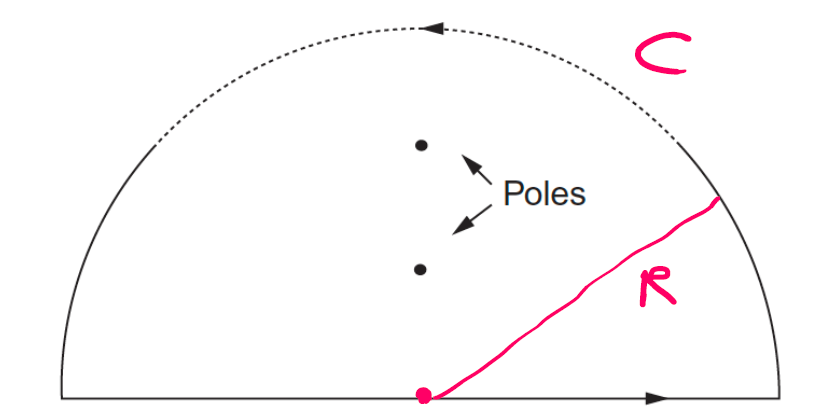
\includegraphics[width=0.5\linewidth]{fig37.png}
\end{figure}

\newpage

\noindent
\textbf{Contribution to the integral from the arc of semi circumference when $R \rightarrow \infty$}

\noindent
Setting $z = Re^{i \theta}$ on the path $C$:
\begin{align*}
    \lim_{R \to \infty} \left| \int_{C} f(z) \, dz \right|
&\leq \int_{\theta_1}^{\theta_2} \lim_{R \to \infty} \left| f\left( R e^{i\theta} \right) i R e^{i\theta} \right| d\theta\\
&\leq \int_{\theta_1}^{\theta_2} \lim_{R \to \infty} \left| f\left( R e^{i\theta} \right) \right| R \, d\theta
\leq \lim_{R \to \infty} \left| f\left( R e^{i\theta} \right) \right| R \int_{\theta_1}^{\theta_2} d\theta\\
&= (\theta_2 - \theta_1) \lim_{R \to \infty} \left| f(z) \cdot z \right| \to 0
\end{align*}
if $f(z)$ vanish faster than $1/z$ when $|z| \rightarrow \infty$. then:
\begin{equation}
    \oint f(z) \, dz = \lim_{R \to \infty} \int_{-R}^{R} f(x) \, dx + \lim_{R \to \infty} \int_{C} f(z) \, dz = 2\pi i \sum \text{residues (upper half-plane)}
\end{equation}

\noindent
\textbf{Example \#1}
\begin{equation}
    I = \int_0^{\infty} \frac{dx}{1 + x^2} 
= \frac{1}{2} \int_{-\infty}^{+\infty} \frac{dx}{1 + x^2}
\end{equation}
to apply the procedure we need to extend the path to $-\infty<x<+\infty$. Recall the figure of semicircle with poles. Since:
\begin{equation}
    \lim_{|z| \to \infty} z f(z) = \lim_{|z| \to \infty} \frac12 \frac{1}{z (1 + z^2)} = 0
\end{equation}
and is meromorphic with finite poles:
\begin{equation}
    I = \frac{1}{2} \int_{-\infty}^{+\infty} \frac{dx}{1 + x^2}
= \frac{1}{2}(2\pi i) \sum \text{residues of } \frac{1}{1 + z^2}
= \frac{1}{(z+i)(z-i)}
\end{equation}
two poles in $z_1=+i$ and $z_2=-i$, and only $z_1$ is inside the contour. Then:
\begin{equation}
    I = \frac{1}{2} \cdot 2\pi i \cdot \operatorname{Res} \left( \frac{1}{(z+i)(z-i)} \right)_{z=i}
= \frac{1}{2} \cdot 2\pi i \cdot \frac{1}{2i} = \frac{\pi}{2}
\end{equation}
Indeed, we already know that:
\begin{equation}
    \int_0^\infty \frac{dx}{1+x^2} = [\tan^{-1}x]^{\infty}_0 = \frac{\pi}{2}
\end{equation}
\noindent
\textbf{Example \#2}

\noindent
A complex exponential vanishes faster than $1/z$ in one of the two semi-planes. In particular for $a>0$ the integral:
\begin{equation}
    I =\int_{-\infty}^{\infty} f(x) e^{iax}
 dx, \quad \text{can be done extending the path in the Im$(z)>0$ complex plane}
\end{equation}
In particular, the contribution to the integral from the semicircle of radius $R$ is:
\begin{equation}
    I_R = \int_{C(R)} f(z) e^{iaz} \, dz
= \int_{0}^{\pi} f\left(R e^{i \theta} \right) e^{iaR \cos \theta} \cdot e^{-a R \sin \theta} \cdot i R e^{i \theta} \, d\theta
\end{equation}
and
\begin{equation}
    z = Re^{i\theta} \Rightarrow e^{iaz} = e^{iaRe^{i\theta}} = e^{iaR(\cos\theta + i\sin\theta)} = e^{iaR \cos \theta} \cdot e^{-a R \sin \theta}, \quad dz = Re^{i\theta}id\theta
\end{equation}
When $R$ is large enough $|f(z)|<\varepsilon$ and :
\begin{equation}
    |I_R| \leq \varepsilon R \int_{0}^{\pi} e^{-aR \sin \theta} \, d\theta
= 2 \varepsilon R \int_{0}^{\frac{\pi}{2}} e^{-aR \sin \theta} \, d\theta
\end{equation}

\newpage

\noindent
In the interval $0 \leq \theta \leq \pi/2$: $\sin\theta \geq \frac{2}{\pi}\theta$.

\begin{figure}[h]
    \centering
    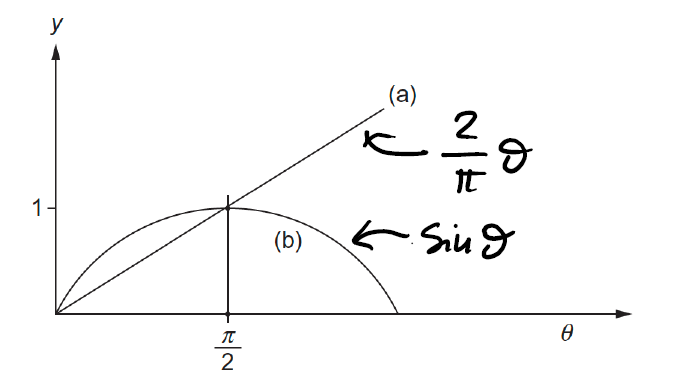
\includegraphics[width=0.5\linewidth]{fig38.png}
\end{figure}

\noindent
then:
\begin{equation}
    |I_R| \leq 2\varepsilon R \int_0^{\pi/2} e^{-2aR\theta/\pi} \, d\theta
= \frac{2\varepsilon R}{-2aR/\pi} \left( e^{-aR} - 1 \right)
= \frac{\varepsilon \pi}{a} \left(1 - e^{-aR}\right)
\leq \frac{\pi}{a} \varepsilon
\end{equation}
so that:
\begin{equation}
    \lim_{R\rightarrow\infty} I_R = 0
\end{equation}

\vspace{2mm}\noindent
\textbf{Jordan’s lemma}
\begin{lemma}[Jordan’s lemma]
    If $\lim_{R\rightarrow\infty} f(z) = 0$ for all $z = Re^{i\theta}$ in the range $0 \leq \theta \leq \pi$, then
    \begin{equation}
        \lim_{R\rightarrow\infty} \int_C e^{iaz} f(z)dz = 0
    \end{equation}
    where $a>0$ and $C$ is a semicircle of radius $R$ in the upper half-plane with center at the origin.
\end{lemma}

\noindent
\textbf{N.B.} The choice of the upper or lower half of the plane depend on the sign of the exponent! Finally:
\begin{equation}
    \int_{-\infty}^{\infty} f(x) e^{iax} \, dx
= 2\pi i \sum \text{residues of } e^{iaz} f(z) \text{ (upper half-plane)} \quad \boxed{a>0}
\end{equation}
\textbf{Example}
\begin{align*}
    I &= \int_0^\infty \frac{\cos x}{x^2 + 1} \, dx
= \int_0^\infty \frac{e^{ix} + e^{-ix}}{2} \frac{dx}{x^2 + 1}\\
&= \frac{1}{2} \int_0^\infty \frac{e^{ix}}{x^2 + 1} \, dx
+ \frac{1}{2} \int_0^\infty \frac{e^{-ix}}{x^2 + 1} \, dx
= \frac{1}{2} \int_0^\infty \frac{e^{ix}}{x^2 + 1} \, dx
+ \frac{1}{2} \int_0^\infty \frac{e^{ix}}{(-x)^2 + 1} \, d(-x)\\
&= \frac{1}{2} \int_{-\infty}^{+\infty} \frac{e^{ix}}{x^2 + 1} \, dx
= \frac{1}{2} \cdot 2\pi i \cdot \operatorname{Res} \left( \frac{e^{ix}}{x^2 + 1}, x = i \right) = \frac12 \cdot 2\pi i \frac{e^{-1}}{2i} = \frac{\pi}{2e}
\end{align*}

\vspace{2mm}\noindent
\textbf{Singularity on the contour of integration}
\begin{align*}
    I &= \int_0^\infty \frac{\sin x}{x} \, dx
= \int_0^\infty \frac{e^{ix} - e^{-ix}}{2i x} \, dx\\
&= \frac{1}{2i} \int_0^\infty \frac{e^{ix}}{x} \, dx
- \frac{1}{2i} \int_0^\infty \frac{e^{-ix}}{x} \, dx
= \frac{1}{2i} \int_0^\infty \frac{e^{ix}}{x} \, dx
- \frac{1}{2i} \int_0^{-\infty} \frac{e^{-i(-x)}}{(-x)} \, d(-x)\\
&= \frac{1}{2i} \int_{-\infty}^{\infty} \frac{e^{ix}}{x}dx
\end{align*}
\textcolor{red}{Diverges in $x=0$! need to calculate the Cauchy principal value:}
\begin{equation}
    I \rightarrow \fint_{-\infty}^{\infty} \frac{e^{ix}}{x}dx
\end{equation}

\newpage
\noindent
We must draw a contour that avoids the singularity in $z=0$. On such contour the identity holds:
\begin{equation}
    \oint \frac{e^{iz}}{2i z} \, dz
= \fint_{-\infty}^{+\infty} \frac{e^{ix}}{2i x} \, dx
+ \lim_{r \to 0} \int_{C_r} \frac{e^{iz}}{2i z} \, dz
+ \lim_{R \to \infty} \int_{C_R} \frac{e^{iz}}{2i z} \, dz
= I + I(C_r) + I(C_R)
\end{equation}

\begin{figure}[h]
    \centering
    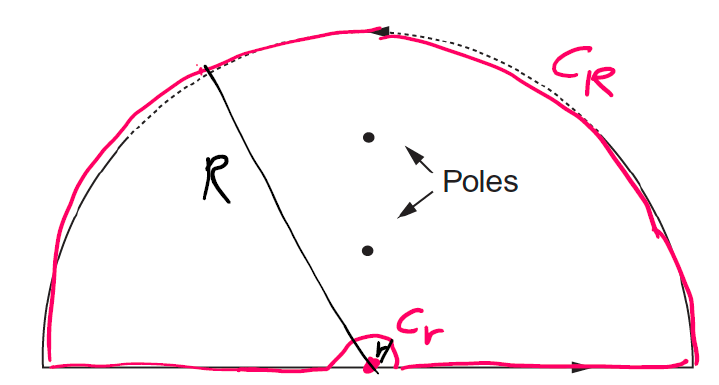
\includegraphics[width=0.5\linewidth]{fig39.png}
\end{figure}

\noindent
By Jordan’s lemma, $I(C_R) \rightarrow 0$ for $R \rightarrow \infty$, while:
\begin{equation}
    I(C_r) = 2\pi i \times \underbrace{\left( -\frac12 \right)}_{(\text{cf})} \text{Res} \left\{ \frac{e^{iz}}{2iz} \right\}_{z=0} = \frac{-2\pi i }{2 \times 2i} = -\frac{\pi}{2}
\end{equation} 
(cf): contributes 1/2 of the residue, minus sign because clockwise. Since the path contains no singularities the integral along to total contour is zero. So:
\begin{equation}
    \oint \frac{e^{iz}}{2i z} \, dz = 0 
= \fint \frac{e^{ix}}{2i x} \, dx 
- \frac{\pi}{2}
\quad \Rightarrow \quad 
\int_0^{\infty} \frac{\sin x}{x} \, dx = \frac{\pi}{2}
\end{equation}

\section{Handout 06}

\noindent
\large\textbf{Branch points}

\normalsize
\noindent
\textbf{Example \#1}
\begin{equation}
    I = \int_0^{\infty} \frac{z^p}{z^2 + 1} \, dz \quad \text{with} \quad 0 < p < 1
\end{equation}
if $p$ is real $z=0$ is a branch point, i.e. the function $x^p$ has infinite values. Need to put a branch cut, and to consider a branch of $x^p$ where it is single valued.

\begin{figure}[h]
    \centering
    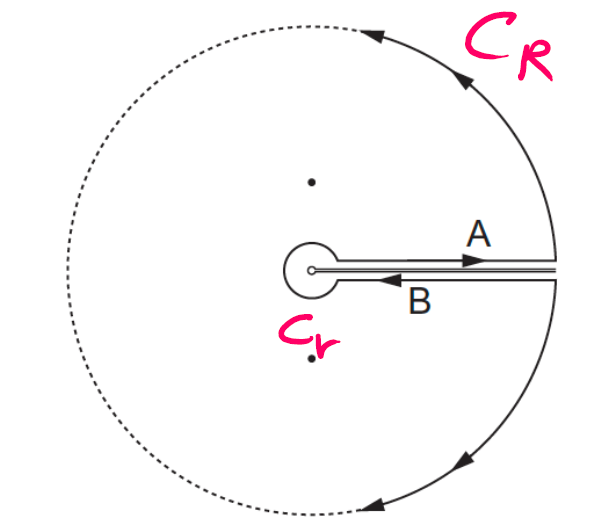
\includegraphics[width=0.35\linewidth]{fig40.png}
\end{figure}

\noindent
\textbf{N.B.} In this branch, when writing $z=re^{i\theta}$ the argument $\theta$ must be in the interval $0<\theta<2\pi$. In other words, it will be \textbf{FORBIDDEN} to extend $\theta$ outside that range. For instance, for periodic functions we are familiar to think that $\theta =-\pi/2$ and $\theta =3\pi/2$ are interchangeable, but now it is no longer true.

\newpage

\begin{equation}
    \oint \frac{z^p dz}{z^2 + 1} = I(C_R) + I(C_r) + I_A + I_B
\end{equation}
for $R\rightarrow \infty$ and for $r \rightarrow 0$ both $I(C_R)$ and $I(C_r)$ vanish. Then:
\begin{equation}
    \oint \frac{z^p dz}{z^2 + 1} = I_A + I_B = (1-e^{2p \pi i})I = 2\pi i \sum_{z_i = \pm i} \text{Res} \left\{ \frac{z^p}{(z+i)(z-i)} \right\}
\end{equation}
with:
\begin{equation}
    I_A = I = \int_0^\infty \frac{x^p dx }{x^2 + 1} \quad \text{(in the limit $r \rightarrow 0$)}
\end{equation}
on the other hand, on path $B$ we have to write: $z = re^{2\pi i }$
\begin{figure}[h]
    \centering
    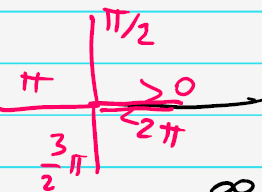
\includegraphics[width=0.25\linewidth]{fig41.png}
\end{figure}
\begin{equation}
    I_B = \int_\infty^0 \frac{(re^{i2\pi})^p e^{i2\pi}dr}{r^2 + 1} = -e^{2p\pi i }\int_0^\infty \frac{r^p dr}{r^2 + 1 } = -e^{2p\pi i}I
\end{equation}
Finally:
\begin{align*}
    \oint \frac{z^p}{z^2 + 1} \, dz 
&= 2\pi i \left[ 
\lim_{z \to e^{i\frac{\pi}{2}}} \cancel{(z-i)}\frac{z^p}{(z+i)\cancel{(z-i)}}
+ \lim_{z \to e^{\frac{3}{2}i\pi}} \cancel{(z+i)} \frac{z^p}{(z-i)\cancel{(z+i)}}
\right]\\
&= 2\pi \cancel{i} \left[ \frac{e^{i\frac{\pi}{2}p}}{2\cancel{i}} + \frac{e^{i\frac{3\pi}{2}p}}{-2\cancel{i}} \right] 
= \left(1 - e^{2\pi pi} \right) I
\end{align*}
from this relation we can solve for $I$!
\begin{equation}
    I = \pi \cdot \frac{e^{i\pi p} \left(e^{-i\frac{\pi p}{2}} - e^{i\frac{\pi p}{2}} \right) / 2i}
{e^{i\pi p} \left(e^{-i\pi p} - e^{i\pi p} \right) / 2i}
= \pi \cdot \frac{\sin\left( \frac{\pi p}{2} \right)}{\sin(\pi p)} = \frac{\pi \cancel{\sin\frac{\pi}{2}p}}{2 \cancel{\sin\frac{\pi}{2}p} \cos\frac{\pi}{2}p }
= \frac{\pi}{2 \cos\left( \frac{\pi p}{2} \right)}
\end{equation}

\noindent
\textbf{Example \#2}
\begin{equation}
    I = \int_0^\infty \frac{dx}{x^3 + 1 } 
\end{equation}
the function is not even, cannot extend the integral to $-\infty < x < +\infty$. How to close the contour path?
\begin{figure}[h]
    \centering
    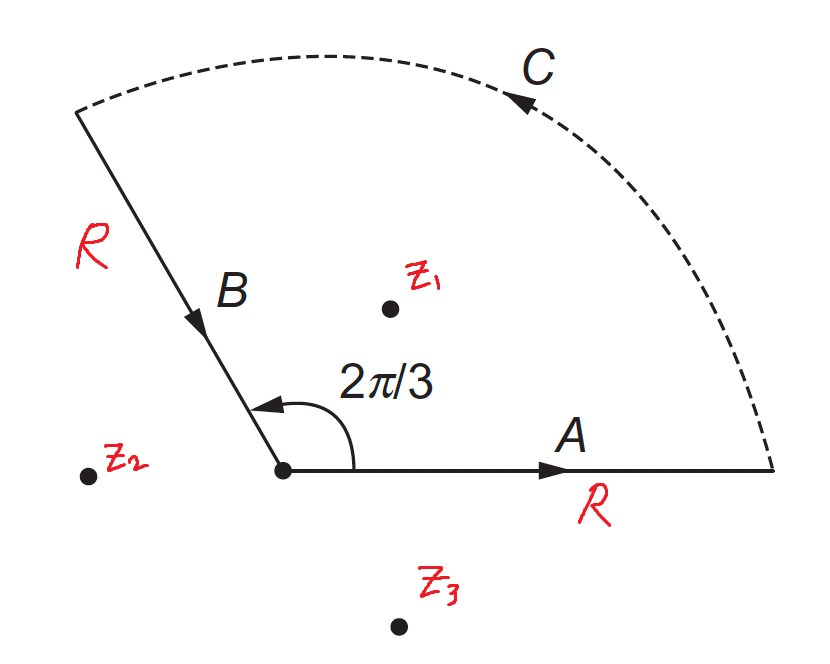
\includegraphics[width=0.4\linewidth]{fig42.png}
\end{figure}

\newpage
\noindent
Exploit the fact that $(e^{2\pi i /3})^3 = 1$ and close the path along segment $B$, where $z=re^{2\pi i /3}$. In particular:
\begin{equation}
    I_a = \int_A \frac{dz}{z^3 +1 } = I, \quad I_B = \int_B \frac{d(e^{2\pi i /3})}{(re^{2\pi i /3})^3 + 1} = e^{2\pi i /3} \int_\infty^0 \frac{dr}{r^3+1} = e^{2\pi i /3}I
\end{equation}
so $I_B$ is not exactly equal to $I$ but proportional to it. Then can set up the contour integral, that will depend on $I$:
\begin{equation}
    \oint_C \frac{dz}{z^3 + 1} = I_A + I_B + I_C
\end{equation}
with:
\begin{equation}
    I_A = \lim_{R \rightarrow \infty} I_A(R)=I
\end{equation}
\begin{equation}
    I_B = \lim_{R \rightarrow \infty} I_B(R)=-e^{2\pi i /3} I
\end{equation}
\begin{equation}
    I_C = \lim_{R \rightarrow \infty} I_C(R)=0
\end{equation}
$1/(z^3 + 1)$ goes to zero faster than $1/z$ for $|z| \rightarrow \infty$. Then:
\begin{equation}
    (1-e^{2\pi i /3})I = 2\pi i \sum_{z_i} \text{Res} \left\{ \frac{1}{z^3 +1} \right\}_{z_i} \quad (\text{inside $C$)}
\end{equation}
the function $1/(z^3 + 1)$ has three simple poles in $z_1 = e^{i\pi /3}$, $z_2 = -1 = e^{i\pi}$, $z_3 = e^{5i\pi/3}$. Only $z$, is inside the contour, so:
\begin{align*}
    \left(1 - e^{-2\pi i / 3} \right) I
&= 2\pi i \cdot \text{Res}\left( \frac{1}{z^3 + 1} \right)_{z_1} = 2\pi i \cdot \lim_{z \to z_1} \frac{z - z_1}{z^3 - 1} \rightarrow \frac{0}{0} \ \ \text{(Use L' Hospital)}\\
&= 2\pi i \lim_{z \rightarrow z_1} \frac{\frac{d}{dz} (z-z_1)}{\frac{d}{dz} (z^3 - 1)} = 2\pi i \lim_{z \rightarrow z_1} \frac{1}{3z^2} = \frac{2\pi i}{3z_1 ^2} = 2\pi i \left( \frac{1}{3 e^{2\pi i /3}} \right)
\end{align*}
So:
\begin{equation}
    \left(1 - e^{2\pi i/3}\right) I = 2\pi i \left( \frac{1}{3 e^{2\pi i/3}} \right) \Rightarrow \left(e^{\pi i/3} - e^{-\pi i/3}\right) I = 2\pi i \cdot \left( -\frac{1}{3} \right)
\end{equation}
hence:
\begin{equation}
    I = \frac{\pi}{3\sin{(\pi/3)}} = \frac{2\pi}{3\sqrt{3}}
\end{equation}
\noindent
\textbf{Example \#3}
\begin{equation}
    I = \int_0^\infty \frac{\ln{x}}{x^3 + 1} dx
\end{equation}
need to avoid the branch point $z=0$ with a small circular detour as in the plot. The integrand as again three poles in $z_1 = e^{i\pi/3}$, $z_2 = -1=  e^{i\pi}$, $z_3 = e^{-i\pi/3}$ with only $z_1$ inside the contour. (keep the branch cut of the logarithm out of the way choosing a direction outside the contour) Then:
\begin{equation}
    \oint \frac{\ln{z}}{z^3 + 1}dz = I_A + I_B + I_C, \quad I_{A,B,C} = \lim_{R \rightarrow \infty} I_{A,B,C} (R), \quad I_A = I, \ \ I_C = 0
\end{equation}

\begin{figure}[h]
    \centering
    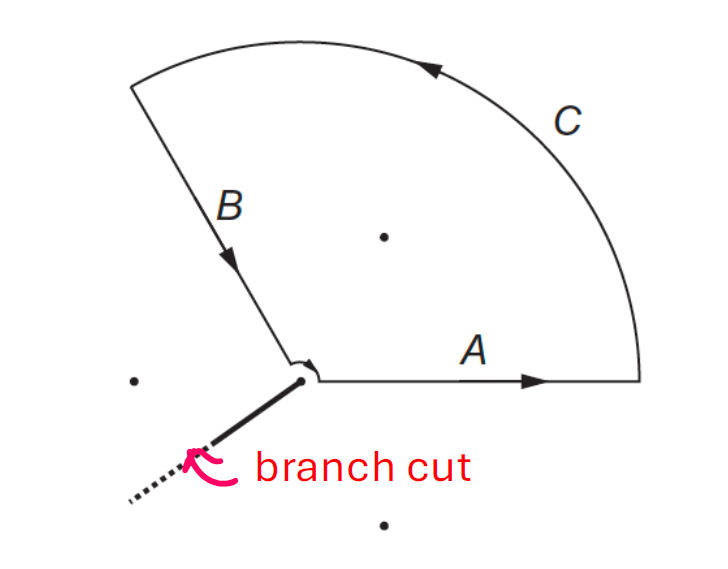
\includegraphics[width=0.35\linewidth]{fig43.png}
\end{figure}

\newpage

\begin{align*}    
    I_B &= \int_B \frac{\ln z \, dz}{z^3 + 1}
= \int_{\infty}^{0} \frac{\ln\left(r e^{2\pi i / 3}\right)}{\left(r e^{2\pi i / 3}\right)^3 + 1} \, d\left(r e^{2\pi i / 3}\right) \quad \text{(on path $B$ one has $z = re^{2\pi i / 3}$)}\\
& = \int_{\infty}^{0} \frac{\ln r + \frac{2\pi i}{3}}{r^3 + 1} \cdot e^{2\pi i / 3} \, dr
= -e^{2\pi i / 3} I -\frac{2\pi i }{3} e^{2\pi i / 3} \underbrace{\int_0^\infty \frac{dr}{r^3 + 1}}_{\text{we will calculate it}}
\end{align*}
value of the last integral:
\begin{equation}
    \int_0^\infty \frac{dr}{r^3 + 1} = \frac{2\pi}{3\sqrt{3}}
\end{equation}
so:
\begin{equation}
    I_B = - e^{2\pi i / 3} I - \frac{2\pi i }{3} e^{2\pi i / 3} \cdot \frac{2\pi}{3\sqrt{3}}
\end{equation}
\textbf{Path $C$}: along path $C$ one has $z = re^{i\theta}$ with $0<\theta<2\pi/3$

\begin{figure}[h]
    \centering
    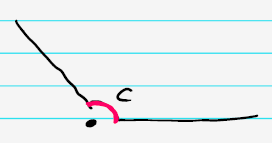
\includegraphics[width=0.25\linewidth]{fig44.png}
\end{figure}
\begin{equation}
    I_C = \lim_{r \to 0} \int_{0}^{\frac{2}{3}\pi} \frac{\ln\left(r e^{i \theta}\right)}{1 + r^3 e^{3i \theta}} \cdot i r e^{i \theta} \, d\theta \to 0
\end{equation}
because: $\lim_{r\rightarrow0} r\ln{r} = 0$, summarizing:
\begin{equation}
    \oint_C \frac{\ln z \, dz}{z^3 + 1}
= I_A + I_B + I_C
= \left(1 - e^{\frac{2\pi i}{3}}\right) I
- \frac{2\pi i}{3} e^{\frac{2\pi i}{3}} \left( \frac{2\pi}{3\sqrt{3}} \right)
= 2\pi i \, \text{Res} \left\{ \frac{\ln z}{z^3 + 1} \right\}_{z = z_1}
\end{equation}
The last ingredient is the calculation of the residue:
\begin{equation}
    \operatorname{Res} \left\{ \frac{\ln z}{z^3 + 1} \right\}_{z_1 = e^{i \pi / 3}} 
= \lim_{z \to z_1} \frac{(z - z_1) \ln z}{z^3 + 1}
= \left. \frac{\ln z}{3z^2} \right|_{z = e^{i \pi / 3}} = \frac{i \pi / 3}{3 e^{i 2\pi / 3}} = \left( \frac{\pi i}{9} \right) e^{-i \frac{2\pi}{3}}
\end{equation}
so, finally:
\begin{equation}
    \left(1 - e^{\frac{2\pi i}{3}}\right) I 
- \frac{2\pi i}{3} e^{\frac{2\pi i}{3}} \left( \frac{2\pi}{3\sqrt{3}} \right) 
= 2\pi i \left( \frac{\pi i}{9} \right) e^{-i \frac{2\pi}{3}}
\end{equation}
to simplify use:
\begin{equation}
    e^{\pm \frac{2\pi i}{3}} = \cos\left(\frac{2\pi}{3}\right) \pm i \sin\left(\frac{2\pi}{3}\right)
= -\frac{1}{2} \pm i \frac{\sqrt{3}}{2}
\end{equation}
hence:
\begin{equation}
   \left(1 - e^{\frac{2\pi i}{3}}\right) I - \frac{2\pi i}{3} e^{\frac{2\pi i}{3}} \left( \frac{2\pi}{3\sqrt{3}} \right) = \left(2\pi i\right) \left(\frac{\pi i}{9}\right) e^{-i\frac{2\pi}{3}}
\end{equation}
\begin{align}
    \left[ 1 - \left( -\frac{1}{2} + i\frac{\sqrt{3}}{2} \right) \right] I - \frac{\cancel{2}\pi i}{3} \left( -\frac{1}{\cancel{2}} + i\frac{\sqrt{3}}{\cancel{2}} \right) \left( \frac{2\pi}{3\sqrt{3}} \right)
= \cancel{2}\pi i \left( \frac{\pi i}{9} \right) \left( -\frac{1}{\cancel{2}} - i\frac{\sqrt{3}}{\cancel{2}} \right)
\end{align}
\begin{equation}
    \left( \frac{3}{2} - i\frac{\sqrt{3}}{2} \right) I
= \frac{\pi^2}{9} \left( 1 + i\sqrt{3} \right)
+ \frac{2\pi^2 i}{9\sqrt{3}} \left( -1 + i\sqrt{3} \right)
= \frac{\sqrt{3}}{2} (\sqrt{3} - i) I
\end{equation}
\begin{equation}
    I = \left[ \frac{\pi^2}{9} (1 + i\sqrt{3}) + \frac{2\pi^2 i}{9\sqrt{3}} (-1 + i\sqrt{3}) \right] /  \frac{\sqrt{3}}{2}(\sqrt{3}-i) = \frac{\pi^2}{9}
\left[
\frac{1 + i\sqrt{3} + \frac{2 i}{\sqrt{3}} (-1 + i\sqrt{3})}
{\frac{\sqrt{3}}{2} (\sqrt{3} - i)}
\right]
\end{equation}
\newpage
\begin{align}
        I &= \frac{\pi^2}{9} \cdot \frac{1 + i\sqrt{3} - \frac{2}{\sqrt{3}} i - 2}{\frac{\sqrt{3}}{2} (\sqrt{3} - i)}
= \frac{\pi^2}{9} \cdot \frac{-1 + \left(\sqrt{3} - \frac{2}{\sqrt{3}} \right) i}{\frac{\sqrt{3}}{2} (\sqrt{3} - i)}\\
&= \frac{\pi^2}{9} \frac{-1 + \frac{1}{\sqrt{3}}i}{\frac{\sqrt{3}}{2}(\sqrt{3} - i)} = \frac{\pi^2}{9} \frac{1}{\sqrt{3}} \frac{-\sqrt{3}+i}{\frac{\sqrt{3}}{2} (\sqrt{3} - i)} = \frac{\pi^2}{9} \cdot \frac23 (-1) = -\frac{2\pi^2}{27}
\end{align}
\begin{equation}
    I = \int_0^\infty \frac{\ln{x}}{x^3 + 1}dx = -\frac{2\pi^2}{27}
\end{equation}
\underline{Sometimes branch cuts are so useful that it can be a good idea to add one!}

\noindent
Let's calculate again:
\begin{equation}
    I = \int_0^\infty \frac{dx}{x^3 + 1}
\end{equation}
let’s set up a similar integral, where we add a function with a branch cut:
\begin{equation}
    \oint_C \frac{\ln z \, dz}{z^3 + 1} = I_A + I_B + \cancel{I_C}
\end{equation}
on the path $C$ in the plot
\begin{equation}
    I_A = \int_A \frac{\ln{z}dz}{z^3 + 1} = \int_0^\infty \frac{\ln{x}dx}{x^3+1}
\end{equation}
\begin{figure}[h]
    \centering
    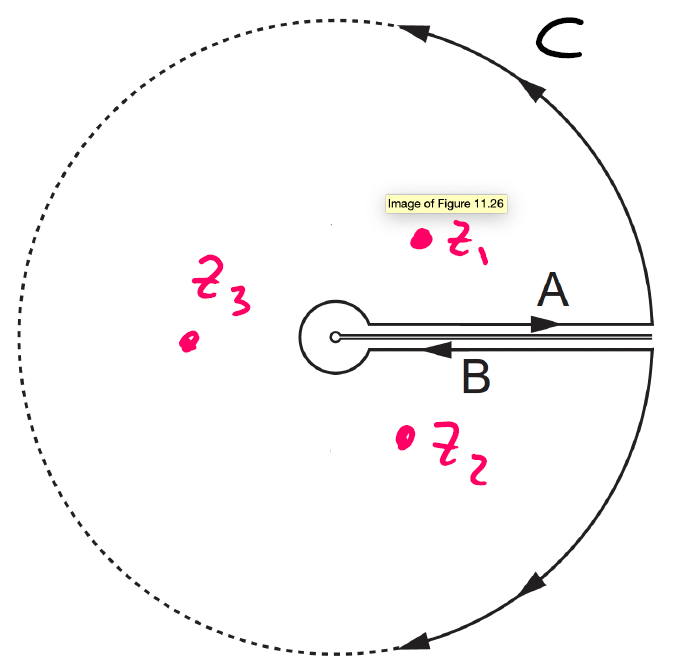
\includegraphics[width=0.35\linewidth]{fig45.png}
\end{figure}

\noindent
due to the cut $0<\theta<2\pi$ on $B$ one has $z = re^{2\pi i }$ so:
\begin{equation}
    I_B = \int_{B} \frac{\ln z \, dz}{z^3 + 1}
= \int_{\infty}^{0} \frac{\ln(re^{2\pi i}) \, e^{2\pi i} \, dr}{(re^{2\pi i})^3 + 1}
= \int_{\infty}^{0} \frac{(\ln x + 2\pi i) \, dx}{x^3 + 1}
\end{equation}
combining the two the logarithmic terms cancel
\begin{align*}
    &\oint_C \frac{\ln z \, dz}{z^3 + 1}
= I_A + I_B
= \cancel{\int_0^\infty \frac{\ln x \, dx}{x^3 + 1}}
+ \cancel{\int_\infty^0 \frac{\ln x \, dx}{x^3 + 1}}
+ 2\pi i \int_\infty^0 \frac{dx}{x^3 + 1}\\
&\Rightarrow \oint_C \frac{\ln z \, dz}{z^3 + 1}
= -2\pi i I
= 2\pi i \sum_{z_i = \text{poles}} \operatorname{Res} \left( \frac{\ln z}{z^3 + 1} \right)_{z_i}
\end{align*}
now all poles $z_1 = e^{i\pi/3}$, $z_2 = e^{i\pi}$, $z_3 = e^{5\pi i/3}$ are inside $C$. (\textbf{N.B.} $z_3$ is NOT $e^{-i\pi/3}$ due to the cut)

\newpage

\[
\operatorname{Res} \left( \frac{\ln z}{z^3 + 1}  \right)_{z = z_1}
= \ln z_1 \cdot \frac{1}{3 z_1^2}
= \ln \left( e^{i\pi/3} \right) \cdot \frac{1}{3 e^{2i\pi/3}}
= \frac{i\pi}{3} \cdot \frac{1}{3 e^{2i\pi/3}} \equiv R_1
\]

\[
\operatorname{Res} \left( \frac{\ln z}{z^3 + 1}  \right)_{z = e^{i\pi}}
= i\pi \cdot \frac{1}{3 e^{6\pi i / 3}} \equiv R_2
\]

\[
\operatorname{Res} \left( \frac{\ln z}{z^3 + 1}  \right)_{z = e^{5\pi i / 3}}
= \frac{5\pi i}{3} \cdot \frac{1}{3 e^{10\pi i / 3}} \equiv R_3
\]

\begin{equation}
    \Rightarrow -(2\pi i) I = 2\pi i \left( R_1 + R_2 + R_3 \right)
\end{equation}

\begin{equation}
    \Rightarrow I = -\left( R_1 + R_2 + R_3 \right)
= -\frac{\pi i}{9} \left( e^{-2\pi i / 3} + 3 + 5e^{2\pi i / 3} \right) 
\quad \left( -\frac{10\pi}{3} = \frac{2\pi}{3} - 4\pi \right)
\end{equation}

\begin{equation}
    e^{-2\pi i / 3} = \cos\left(- \frac{2\pi}{3} \right) + i \sin\left(- \frac{2\pi}{3} \right)
= -\frac{1}{2} - \frac{\sqrt{3}}{2} i \ ; \quad e^{2\pi i / 3} = -\frac{1}{2} + \frac{\sqrt{3}}{2} i
\end{equation}

\begin{equation}
    I = -\frac{\pi i }{9} \left( \cancel{-\frac12} - \frac{\sqrt{3}}{2}i + \cancel{3} -\cancel{\frac52} + \frac52 \sqrt{3}i \right) = -\frac{\pi i}{9} (2\sqrt{3}i) = \frac{2\pi}{3\sqrt{3}}
\end{equation}
\textbf{Exploit periodicity:}
\begin{equation}
    I = \int_0^\infty \frac{xdx}{\sinh{x}}
\end{equation}
calculate:
\begin{equation}
    \oint_C \frac{zdz}{\sinh{z}} \quad \text{on the contour $C$ in the plot (taking as usual $R \rightarrow \infty$)}
\end{equation}
\textbf{N.B.} On the imaginary axis the hyperbolic sin $\sinh(z)$ is proportional to the trigonometric sine, $\sinh(ix)=i \sin(x)$, i.e. it is periodic.

\begin{figure}[h]
    \centering
    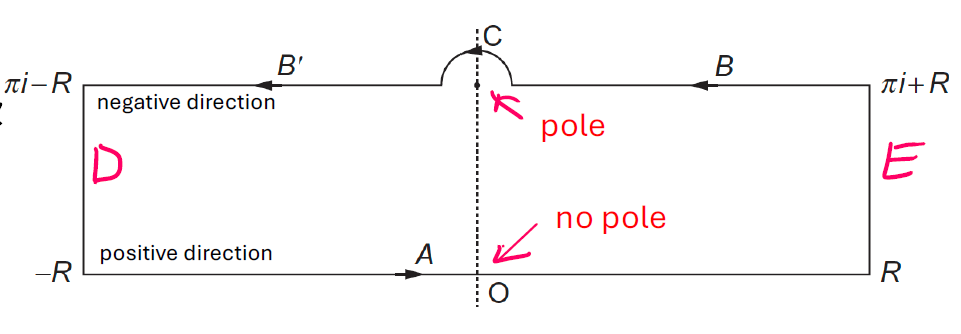
\includegraphics[width=0.65\linewidth]{fig46.png}
\end{figure}

\begin{equation}
    \sinh(x + iy) = \sinh x \cosh(iy) + \cosh x \sinh(iy) + \sinh x \cos y + i \cosh x \sin y \quad \cosh x > 0 \quad \forall x \in \mathbb{R}
\end{equation}
The poles of $z/\sinh{z}$ are in the zeros of $\sinh{z}$, $z=n\pi i$ ($n \in \mathbb{Z}$) with the exception of $z=n=0$, where:
\begin{equation}
    \lim_{z \rightarrow 0} \frac{z}{\sinh{z}}=1, \quad I_A = \int_A \frac{zdz}{\sinh{z}} = 2I, \quad \text{(the integrand is an even function)}
\end{equation}
using:
\begin{equation}
    \sinh(x + i\pi) = \sinh x \cosh(i\pi) + \cosh x \sinh(i\pi) = \sinh x \cos \pi + \cancel{ i \cosh x \sin \pi} = - \sinh x D
\end{equation}
\begin{equation}
    I_{B'} = \int_{-\infty}^{0-\varepsilon} \frac{(x + i\pi)dx}{\sinh{(x+i\pi)}} = \int_{0+\varepsilon}^{\infty} \frac{(x+i\pi)dx}{\sinh{x}}
\end{equation}

\newpage

\noindent
so:
\begin{equation}
    \int_{B+B'} \frac{zdz}{\sinh{z}} = \fint_{-\infty}^\infty \frac{x + i\pi}{\sinh{x}}dx \quad \text{principal value, cut out contour around
singularity}
\end{equation}
Notice that $x/\sinh(x)$ is even but $i\pi/\sinh(x)$ (the second term in the integral) is odd, so it does not contribute. Then:
\begin{equation}
    \fint_{-\infty}^\infty \frac{x dx}{\sinh{x}} = 2I
\end{equation}
and applying the residue theorem:
\begin{align}
    \int_{A+B+B'+C+E} \frac{zdz}{\sinh{z}} &= I_A + I_{B+B'} + I_C + \cancel{I_D} + \cancel{I_E} = 2\pi i \ \text{Res} \left\{ \frac{z}{\sinh{z}} \right\}_{z = \pi i }\\
    &\Rightarrow 2I + 2I + \int_C \frac{zdz}{\sinh{z}} =\text{Res} \left\{ \frac{z}{\sinh{z}} \right\}_{z = \pi i }
\end{align}

\begin{equation}
    \text{Res} \left\{ \frac{z}{\sinh{z}} \right\}_{z = \pi i } = \lim_{z \rightarrow \pi i } (z - i\pi) \frac{z}{\sinh{z}} = \lim_{z \rightarrow \pi i } - \frac{\cancel{\sinh{z} }z}{\cancel{\sinh{z}}} = -i\pi
\end{equation}
since:
\begin{align*}
    \lim_{z \rightarrow \pi i } \frac{z-i\pi}{\sinh{(z-i\pi)}} = 1 &\Rightarrow \lim_{z \rightarrow \pi i }(z-i\pi) = \sinh{(z-i\pi)}\\
    &= \sinh{(i\pi)} \cosh{(-i\pi)} + \cosh (i\pi) \sinh(-i\pi)= \sinh (i\pi)   \cos (i\pi) -i \cosh (\pi) \sin (\pi) = -\sinh z
\end{align*}

\begin{figure}[h]
    \centering
    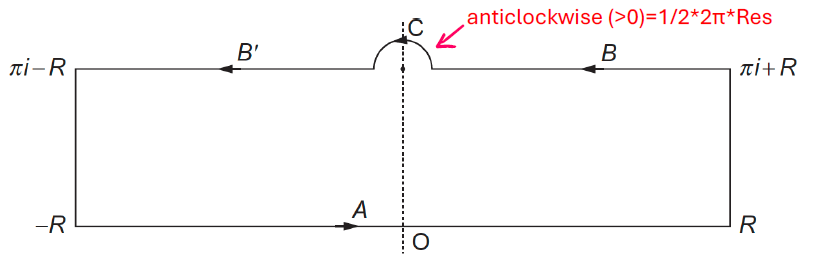
\includegraphics[width=0.7\linewidth]{fig47.png}
\end{figure}

\noindent
Moreover:
\begin{equation}
    I_C = \frac{1}{2} \cdot 2\pi i \cdot \operatorname{Res} \left( \frac{z}{\sinh z} \right)_{ z = i\pi}
= \frac{1}{2} \cdot 2\pi i \cdot (-i\pi) = \pi^2
\end{equation}
And, finally:
\begin{equation}
    \oint_C \frac{z\,dz}{\sinh z} = 4I + \pi^2 = 2\pi i (-i\pi)
\ \ \Rightarrow \ \  I = \frac{2\pi^2 - \pi^2}{4} = \frac{\pi^2}{4}
\end{equation}

\vspace{2mm}\noindent
\textbf{Evaluation of sums of series using residues}

\noindent
The value of a contour integral in the complex plane is given by a sum of residues. If inside the integration path a function has an infinite number of equally spaced residues at $x=n$ ($n$=integer on the real axis) the result of the integral is a series. Indeed, trigonometric functions can be used for this.

\noindent
Consider:
\begin{equation}
    \cot{z} = \frac{\cos z}{\sin z}
\end{equation}
it has poles where $\sin(z)=0$, i.e. $z=n\pi$ with $n$=integer. So: $\cot (\pi z)$. Has poles at $\pi z=n\pi \rightarrow z = z_0 = n$. The residue at $z_n$ is:
\begin{equation}
    \operatorname{Res} \left\{ \cot(\pi z) \right\}_{z = z_n}
= \lim_{z \to z_n} (z - z_n) \cot(\pi z)
= \lim_{z \to z_n} \frac{z - z_n}{\tan(\pi z)}
= \lim_{z \to z_n} \frac{d}{dz}(z - z_n) \cdot \frac{1}{\frac{d}{dz} \tan(\pi z)}
\end{equation}
\begin{equation}
    \operatorname{Res} \left\{ \cot(\pi z) \right\}_{z = z_n} = \lim_{z \to z_n} \frac{1}{(1+\tan^2 \pi z )\pi} = \frac{1}{\pi}
\end{equation}

\newpage

\noindent
In other words:
\begin{equation}
    \operatorname{Res} \left\{\pi  \cot(\pi z) \right\}_{z = z_n} = 1
\end{equation}
This can be directly used to obtain the integral:
\begin{equation}
    I_{\mathcal{N}} = \oint_{C_{\mathcal{N}}(R)} f(z)\, \pi \cot(\pi z)\, dz
\end{equation}
on path $C_{N(R)}$ containing the poles from $–N$ to $+N$.
\begin{figure}[h]
    \centering
    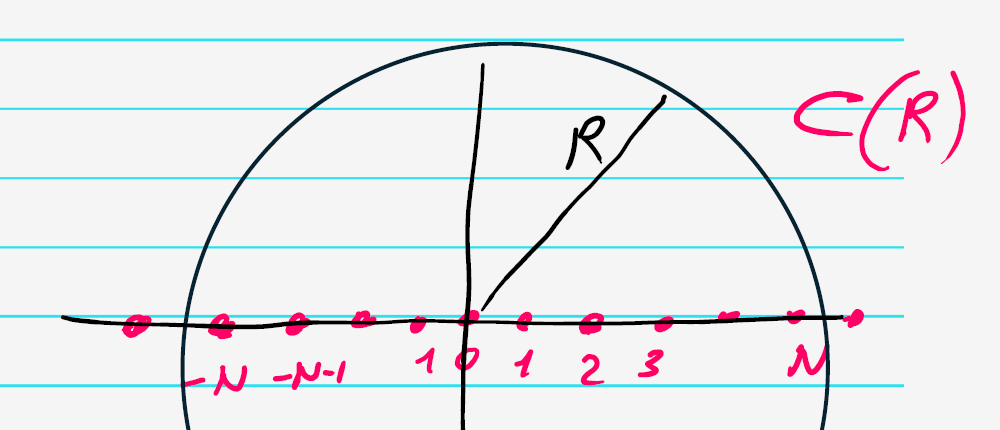
\includegraphics[width=0.5\linewidth]{fig48.png}
\end{figure}

\noindent
Assuming that $f(z)$ is meromorphic and has only isolated poles $z_i$ \underline{\textbf{other than integers}}:
\begin{equation}
    I_{N} = 2\pi i \sum_{M=-N}^{N} f(n) + 2\pi i \sum_{i} \operatorname{Res} \left\{ f(z)\, \pi \cot(\pi z) \right\}_{z = z_i}
\end{equation}
If we allow the radius of $C$ to go to infinity and assume that $zf(z) \rightarrow 0$ for $|z| \rightarrow \infty$:
\begin{equation}
    I_N = \lim_{R\rightarrow \infty} \oint_{C(R)} f(z) \pi  \cot (\pi z) dz = 0
\end{equation}
and:
\begin{align}
    &0 = 2\pi i \sum_{n=-\infty}^{\infty} f(n) + 2\pi i \sum_i \text{Res} \{ f(z) \pi \cot (\pi z) \}_{z=z_i}\\
    & \ \  \Rightarrow \sum_{n = -\infty}^{\infty} = -2 \pi i  \sum_i \text{Res} \{ f(z) \pi \cot (\pi z) \} _{z=z_i}
\end{align}
\textbf{N.B.} The crucial point is that in the right-hand side the sum is over a finite (in general a few) poles, not on an infinite list!

\vspace{3mm}\noindent
\textbf{Example:}
\begin{equation}
    S = \sum_{n=1}^\infty \frac{1}{n^2 + a^2} \quad a\neq \text{integer}
\end{equation}
note also that
\begin{equation}
    S  = \sum_{n = -\infty}^{-1} \frac{1}{n^2 + a^2}
\end{equation}
so:
\begin{equation}
    \sum_{n = -\infty}^{\infty} \frac{1}{n^2 + a^2} = 2S + \frac{1}{a^2}\ \quad (\text{term corresponding to the missing $n=0$})
\end{equation}
Now:
\begin{equation}
    f(z) = \frac{1}{z^2 + a^2} \quad \text{with poles at $z = \pm ia$}
\end{equation}

\newpage

\noindent
So:
\begin{align*}
    \sum_{z_i = \pm i a} \operatorname{Res} \left\{ f(z)\, \pi \cot(\pi z) \right\}_{z = z_i} &= \pi \cot(\pi i a) \lim_{z \to i a} \frac{\cancel{z - i a}}{(z + i a)\cancel{(z - i a)}} 
+ \pi \cot(-\pi i a) \lim_{z \to -i a} \frac{\cancel{z + i a}}{\cancel{(z + i a)}(z - i a)}\\
&=\pi \cot(\pi i a) \frac{1}{2 i a} + \pi \cot(-\pi i a) \frac{1}{-2 i a} 
= \pi \left( \frac{-\cancel{i} \coth(\pi a)}{2 \cancel{i} a} + \frac{\cancel{i} \coth(\pi a)}{-2 \cancel{i} a} \right)
\end{align*}

\begin{equation}
    \cot(\pi i a) = \frac{\cos(i \pi a)}{\sin(i \pi a)} 
= \frac{\cosh(\pi a)}{-\sinh(\pi a)/i} 
= -i \coth(\pi a)
\end{equation}
and,
\begin{equation}
    \cot (-i\pi a) = i \coth (\pi a)
\end{equation}
then:
\begin{equation}
    \sum_{z_i = \pm i a} \operatorname{Res} \left( f(z) \, \pi \cot(\pi z) \right)_{z=z_i} 
= -\frac{\pi}{2a} \coth(\pi a) - \frac{\pi}{2a} \coth(\pi a) 
= -\frac{\pi}{a} \coth(\pi a)
\end{equation}
and finally:
\begin{equation}
    2S + \frac{1}{a^2} = \sum_{n=-\infty}^{+\infty} \frac{1}{n^2 + a^2} 
= - \sum_{z_i = \pm i a} \operatorname{Res} \left( f(z) \, \pi \cot(\pi z) \right)_{z=z_i} 
= \frac{\pi}{a} \coth(\pi a)
\end{equation}
\begin{equation}
    S = \frac{1}{2} \left[ \frac{\pi}{a} \coth(\pi a) - \frac{1}{a^2} \right]
\end{equation}

\vspace{3mm}\noindent
Additional types of summations can be performed if we replace $\cot(\pi z)$ by functions with other regularly repeating patterns of residues. For example, $\pi \csc(\pi z)$ has residues for integer $z$ that alternate in sign between -1 and +1; $\pi \tan(\pi z)$ has residues that are all +1, but occur at the points $n+1/2$. And $\pi \sec(\pi z)$ has residues $\pm1$ at the half-integers with a sign alternation.

\begin{figure}[h]
    \centering
    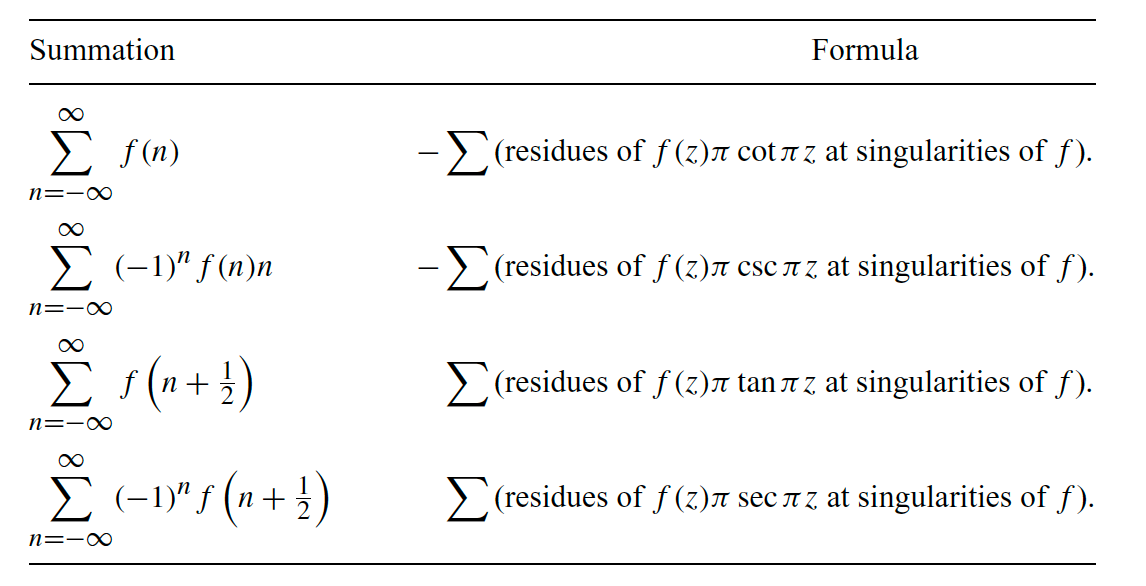
\includegraphics[width=0.85\linewidth]{fig49.png}
\end{figure}

%휴 중간고사 범위까지 끝났다 tlqkf...

\newpage

\section{Handout 07}

\large
\begin{center}
    \textbf{Partial differential equations (PDEs)}
\end{center}

\normalsize
\noindent
PDEs involve derivatives with respect to more than one independent variable. So the dependent variable will contain partial derivatives.

\vspace{2mm}\noindent
Example: 2 variable PDE
\begin{itemize}
    \item Independent variables: $x, y$
    \item Dependent variable: $\varphi(x, y)$
    \item The PDE will contain:
    $$\frac{\partial \varphi}{\partial x} = \text{derivative of $\varphi$ with respect to $x$ keeping $y$ fixed (i.e. treating it as a constant)}$$
    $$\frac{\partial \varphi}{\partial y} = \text{derivative of $\varphi$ with respect to $y$ keeping $x$ fixed (i.e. treating it as a constant)}$$
    \item Plus higher derivatives, including mixed derivatives:
    $$\frac{\partial^2 \varphi}{\partial x^2} \equiv \frac{\partial}{\partial x} \left( \frac{\partial \varphi}{\partial x} \right), \quad
\frac{\partial^2 \varphi}{\partial y^2}, \quad
\frac{\partial^2 \varphi}{\partial x \partial y} \equiv \frac{\partial}{\partial x} \left( \frac{\partial \varphi}{\partial y} \right) =
\frac{\partial^2 \varphi}{\partial y \partial x}, \quad
\frac{\partial^3 \varphi}{\partial y^3}, \quad
\frac{\partial^3 \varphi}{\partial^2 y \partial x}, \ \ \text{etc..}$$
\end{itemize}

\noindent
Important: like ordinary derivatives, also partial derivatives are linear
$$\frac{\partial}{\partial x} \left[ a\, \varphi(x, y) + b\, \gamma(x, y) \right]
= a \frac{\partial \varphi(x, y)}{\partial x} + b \frac{\partial \gamma(x, y)}{\partial x}$$

\noindent
“the derivative of the linear combination is the linear combination of the derivative”. Then we can see ODEs as the action of a linear operator $\mathcal{L}$ on the function $\phi$:
\begin{equation*}
    \mathcal{L} = \frac{\partial^2}{\partial x^2} -xy^2 \frac{\partial}{\partial y}, \quad F=  xy \ \ \Rightarrow \ \ \boxed{\mathcal{L} \varphi = F \longleftrightarrow \frac{\partial^2 \varphi}{\partial x^2} -xy^2\frac{\partial \varphi}{\partial y} = xy}
\end{equation*}
source term: if it is zero the PDE is homogeneous, otherwise it is inhomogeneous

\noindent
Since the dynamics of many physical systems involve just two derivatives differential equations of second order occur most frequently in physics (in classical mechanics Newton’s law involves acceleration -second derivative with respect to time-, in quantum mechanics the momentum operator is $\hat{p} = -i \vec{\nabla}$ so the the kinetic energy operator $p^2 / 2m$ appearing in the Hamiltonian is $K = - (\nabla^2 / 2m)$ etc...

\vspace{2mm} \noindent
\textbf{Plan:}

\begin{itemize}
    \item Will mainly concentrate on \textbf{homogeneous PDE}s (extension to inhomogeneous PDEs with a nonvanishing source term postponed to the lectures on Green’s functions)
    \item Begin considering \textbf{first-order PDE}s to introduce some of the most important principles
    \item Move-on to classify the properties of \textbf{second-order PDE}s
    \item Powerful method to solve homogeneous PDE’s: \textbf{separation of variables}
\end{itemize}

\newpage
\noindent
First-order homogeneous equations (simplest case, but provide useful insights that apply also to higher-order problems)
\begin{equation}
    \mathcal{L} \varphi(x, y) = a \frac{\partial \varphi(x, y)}{\partial x}
+ b \frac{\partial \varphi(x, y)}{\partial y} = 0
\end{equation}
introduce new coordinates s and t with a linear transformation of the type:
\begin{equation}
    \begin{pmatrix}
s \\
t
\end{pmatrix}
=
M
\begin{pmatrix}
x \\
y
\end{pmatrix}
=
\begin{pmatrix}
\alpha & \beta \\
\gamma & \delta
\end{pmatrix}
\begin{pmatrix}
x \\
y
\end{pmatrix}
\Rightarrow
\begin{cases}
s = \alpha x + \beta y \\
t = \gamma x + \delta y
\end{cases}
\end{equation}
choosing the terms a,b,c,d is such a way that one only one of them (for instance, s) appears in the PDE, while the PDE does not contain derivatives in t (which can then be treated as an external parameter):
\begin{equation}
    \hat{\varphi}(s, t) \equiv \varphi\left[ x(s, t),\, y(s, t) \right]
\end{equation}
Then:
\begin{align}
    \frac{\partial \varphi}{\partial x}
&= \left( \frac{\partial \varphi}{\partial x} \right)_y
= \left( \frac{\partial \varphi}{\partial s} \right)_t \frac{\partial s}{\partial x}
+ \left( \frac{\partial \varphi}{\partial t} \right)_s \frac{\partial t}{\partial x}
= \alpha \left( \frac{\partial \varphi}{\partial s} \right)_t
+ \gamma \left( \frac{\partial \varphi}{\partial t} \right)_s\\
\frac{\partial \varphi}{\partial y}
&= \left( \frac{\partial \varphi}{\partial y} \right)_x
= \left( \frac{\partial \varphi}{\partial s} \right)_t \frac{\partial s}{\partial y}
+ \left( \frac{\partial \varphi}{\partial t} \right)_s \frac{\partial t}{\partial y}
= \beta \left( \frac{\partial \varphi}{\partial s} \right)_t
+ \delta \left( \frac{\partial \varphi}{\partial t} \right)_s
\end{align}
substitute in the equation:
\begin{align}
    a \left[ \alpha \left( \frac{\partial \varphi}{\partial s} \right)_t + \gamma \left( \frac{\partial \varphi}{\partial t} \right)_s \right]
+ b \left[ \beta \left( \frac{\partial \varphi}{\partial s} \right)_t + \delta \left( \frac{\partial \varphi}{\partial t} \right)_s \right]= (a\alpha + b\beta) \frac{\partial \varphi}{\partial s}
+ (a\gamma + b\delta) \frac{\partial \varphi}{\partial t}
= 0
\end{align}
when require $(a\alpha+b\delta = 0)$.

\vspace{2mm}\noindent
Simplest choice: take vector $(\alpha, \beta) = (a, b)$ parallel to $(a,b)$ and vector $(\gamma, \delta) = (-b, a)$ perpendicular to it, so that the coefficient that multiplies $\partial \varphi/ \partial x$ vanishes: when $s = ax + by$, $t = bx - ay$.
\begin{equation}
    \left( a\alpha + b\gamma \right) \frac{\partial \hat{\varphi}}{\partial s}
+ \left( a\gamma + b\delta \right) \frac{\partial \hat{\varphi}}{\partial t} = 0 \quad / \quad (a^2 + b^2 ) \frac{\partial \hat{\varphi}}{\partial s} = 0
\end{equation}
the solution is trivial (any function $f(t)$ that does not depend on s!)
\begin{equation}
    \hat{\varphi} (s,t) = f(t)
\end{equation}
so, using $t = bx-ay$ this means that:
\begin{equation}
\varphi(x, y) = f(bx-ay)
\end{equation}
What the ODE is telling is a that $\varphi$ is any function that depends on $x$ and $y$ only through the combination $bx-ay$. The solution $\varphi$ depends on $t = bx-ay$, which represents line in the $x$, $y$ plane. Soon on that line $\varphi$ is constant:

\begin{figure}[h]
    \centering
    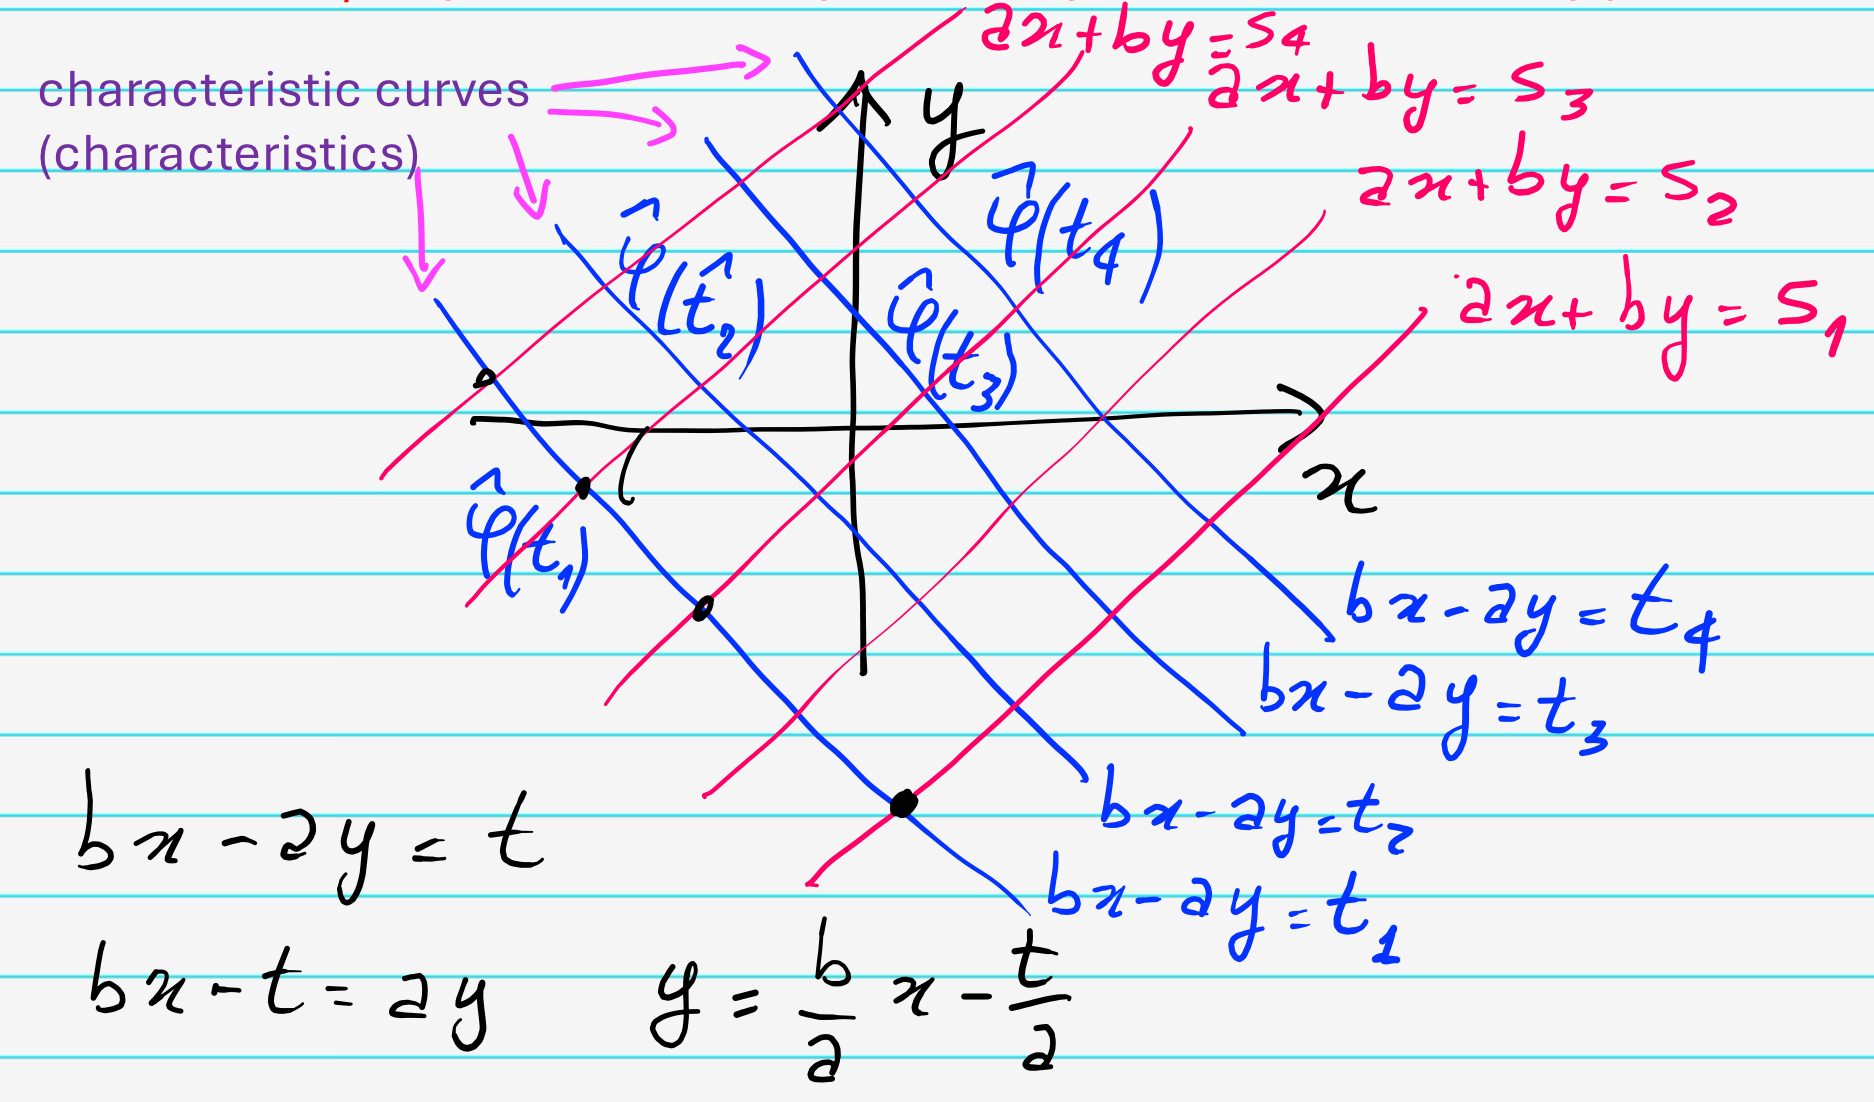
\includegraphics[width=0.5\linewidth]{fig51.jpeg}
\end{figure}

\newpage

\noindent
Remember that we chose the two vector $(a, b)$, and $(-b,a)$ orthogonal, i.e. in the $xy$ plane the lines of constant $s=ax+by$ are orthogonal. The curves at constant $t$ are called \textbf{characteristic curves} or simply \textbf{characteristic}. They are the stream lines of $s$, in the sense that along a given characteristic $t$ is constant and $s$ is changing. 

\noindent
This is a general approach, valid also for more general PDEs: the solutions propagate along characteristic lines, in the sense that on each characteristic line the solution is “in phase” (this is what happens in wave solutions): 

\begin{figure}[h]
    \centering
    \includegraphics[width=0.4\linewidth]{fig52.png}
\end{figure}

\begin{equation}
    \varphi(x,y) = f(t = bx-ay)
\end{equation}

\noindent
\textbf{Boundary condition}

\noindent
Ordinarily, the function $\varphi$ is fixed to some value on a curve (boundary conditions). Suppose we want to solve the PDE assuming that $\varphi = \varphi_0 = 0$ on a certain line.

\begin{figure}[h]
    \centering
    \includegraphics[width=0.4\linewidth]{fig53.png}
\end{figure}

\noindent
On each characteristic that crosses the line $\varphi = \varphi_0$,  but if this is true on a point of the characteristic it is true everywhere. So the only solution is $\varphi(x,y) = \varphi_0 = \text{constant}$.

\noindent
Suppose instead that we parameterize the curve of the boundary condition as $x(l)$ and $y(l)$ and we fix $\varphi_0 [x(l, y(l)]=  \varphi_0(l)$, with $\varphi_0(l)$ a given function (so we know $\varphi_0 (l)$ on the curve $[x_0 (l), y_0 (l)]$.

\begin{figure}[h]
    \centering
    \includegraphics[width=0.6\linewidth]{fig54.png}
\end{figure}

\newpage

\noindent
This in principle allows to know the value of $\varphi(x,y)$ in any point $(x,y)$: it is sufficient to find the value of $l$ that corresponds to the intersection between the characteristic passing through $(x,y)$ and the boundary condition curve $[x(l), y(l)]$. This will determine a value of the parameter $l$. Then $\varphi(x,y) = \varphi_0(l)$.

\vspace{2mm}\noindent
However, suppose that the boundary condition is fixed on a characteristic curve (it will have to be a constant to be consistent, $\varphi_0(l) = K$). Then it will be impossible to determine the value of $\varphi(x,y)$ in a point outside $x_0(l), y_0(l)$.

\vspace{2mm}\noindent
If we know $\varphi(x_0, y_0)$ in a point ($x_0, y_0$) of the boundary condition curve we can determine $\varphi(x,y)$ In a close point outside the boundary condition curve by writing the expansion:

\begin{equation}
    \varphi(x, y) = \varphi(x_0, y_0) + \left. \frac{\partial \varphi}{\partial x} \right|_{x_0, y_0} (x - x_0) + \left. \frac{\partial \varphi}{\partial y} \right|_{x_0, y_0} (y - y_0) + \cdots
\end{equation}
So we need $\partial \varphi / \partial x$ and $\partial \varphi / \partial y$ in $x_0, y_0$.

\noindent
In particular, if we know $\varphi_0(l)$ on the curve $[x(l), y(l)]$ we also know $d\varphi_0/dl$ and $dx/dl$ and $dy/dl$. Then, combining with the PDF we obtain two linear relation for $\partial \varphi / \partial x$ and $\partial \varphi / \partial y$:
\begin{equation}
    \left\{
\begin{aligned}
\frac{d \varphi_0}{d l} &= \frac{\partial \varphi}{\partial x} \frac{d x}{d l} + \frac{\partial \varphi}{\partial y} \frac{d y}{d l} \\
0 &= a \frac{\partial \varphi}{\partial x} + b \frac{\partial \varphi}{\partial y}
\end{aligned}
\right.
\Rightarrow
\begin{pmatrix}
\frac{d x}{d l} & \frac{d y}{d l} \\
a & b
\end{pmatrix}
\begin{pmatrix}
\frac{\partial \varphi}{\partial x} \\
\frac{\partial \varphi}{\partial y}
\end{pmatrix}
=
\begin{pmatrix}
\frac{d \varphi_0}{d l} \\
0
\end{pmatrix}
\end{equation}
The linear system has a solution if the determinant of the matrix does not vanish. However, if $x(l),y(l)$ corresponds to a characteristic:
\begin{equation}
    bx(l) - ay(l) = t_0 \ \ \Rightarrow \ \ b\frac{dx}{dl}-a\frac{dy}{dl} = 0 \ \ \Rightarrow \ \ \frac{dy}{dl} = \frac{b}{a} \frac{dx}{dl}
\end{equation}
and the determinant is:
\begin{equation}
    \left| 
\begin{array}{cc}
\frac{dx}{dl} & \frac{dy}{dl} \\
a & b
\end{array}
\right|
=
\left|
\begin{array}{cc}
\frac{dx}{dl} & \frac{b}{a} \frac{dx}{dl} \\
a & b
\end{array}
\right|
=
\left|
\begin{array}{cc}
\frac{1}{a} \frac{dx}{dl} \cdot a & \frac{1}{a} \frac{dx}{dl} \cdot b \\
a & b
\end{array}
\right|
= 0
\end{equation}
So, as already pointed out, if the boundary condition is set on a characteristic it is not possible to determine the solution outside it.

\vspace{2mm}\noindent
Also, if the boundary condition is set on a curve that intersects the same characteristics more than once (for example twice) this usually leads to an inconsistency unless in both intersections $\varphi_0 (l_1)$ and $\varphi_0 (l_2)$ are equal:

\begin{figure}[h]
    \centering
    \includegraphics[width=0.4\linewidth]{fig55.png}
\end{figure}

\newpage
\noindent
\textbf{Summarizing:}
\begin{enumerate}
    \item If the dependent variable of the PDE is specified along a curve this fixes the value of $\varphi$ at a point of each characteristic that intersects the boundary curve, and hence at all points of each such characteristic;
    \item If the boundary curve is along a characteristic, the boundary condition on it will ordinarily lead to inconsistency, and therefore, unless the boundary condition is redundant (i.e., coincidentally equal everywhere to the solution constructed from the value of at any one point on the characteristic), the PDE will not have a solution;
    \item If the boundary curve has more than one intersection with the same characteristic, this will usually lead to an inconsistency, as the PDE may not have a solution that is simultaneously consistent with the values of $\varphi$ at both intersections; 
    \item Only if the boundary curve is not a characteristic can a boundary condition fix the value of $\varphi$ at points not on the curve. Values of $\varphi$ specified only on a characteristic of the PDE provide no information as to the value of $\varphi$ at points not on that characteristic.
\end{enumerate}

\noindent
\textbf{More general PDE’s}
\begin{equation}
    \mathcal{L} \varphi = a \frac{\partial \varphi}{\partial x} + b \frac{\partial \varphi}{\partial y} + Q(x, y) = F(x, y)
\end{equation}
more complicated than before. But we can use the same change of variable:
\begin{equation}
    \begin{cases}
        s = ax + by \\ t = bx-ay
    \end{cases} \ \ \Rightarrow \ \ x = \frac{as + bt}{a^2 + b^2}, \ \ \frac{bs-at}{a^2 + b^2}
\end{equation}
in terms of $s$ and $t$:
\begin{equation}
    \left( a^2 + b^2 \right) \left( \frac{\partial \varphi}{\partial s} \right)
+ \hat{Q}(s, t) = \hat{F}(s, t)
\end{equation}
with:
\begin{equation}
    \hat{Q}(s, t) = Q\left[ x(s, t),\, y(s, t) \right]
\quad ; \quad
\hat{F}(s, t) = F\left[ x(s, t),\, y(s, t) \right]
\end{equation}

\vspace{2mm}\noindent
\textbf{Example:}
\begin{equation}
    \frac{\partial \varphi}{\partial x} + \frac{\partial \vp}{\partial y} + (x+y) \vp = 0
\end{equation}
\begin{equation}
    \begin{cases}
        s = x+y \\ t = x-y
    \end{cases} \ \ \Rightarrow \ \ \begin{cases}
        2x = s+t\\ 2y = s-t
    \end{cases} \ \ \Rightarrow \ \ \begin{cases}
        x +y = s
    \end{cases}
\end{equation}
\begin{equation}
    \frac{\partial \varphi}{\partial s} \frac{\partial s}{\partial x}
+ \frac{\partial \varphi}{\partial t} \frac{\partial t}{\partial x}
+ \frac{\partial \varphi}{\partial s} \frac{\partial s}{\partial y}
+ \frac{\partial \varphi}{\partial t} \frac{\partial t}{\partial y}
+ s \varphi = 0
\end{equation}
\begin{equation}
    \frac{\partial \varphi}{\partial s}
\cancel{+ \frac{\partial \varphi}{\partial t}}
+ \frac{\partial \varphi}{\partial s}
\cancel{- \frac{\partial \varphi}{\partial t}}
+ s \varphi = 0
\end{equation}
\begin{equation}
    2 \frac{\partial \vp}{\partial s} + s\vp = 0 \quad \textcolor{red}{\text{can be seen as an ODE in a single variable $s$, with $t$ as an external parameter}}
\end{equation}
separable:
\begin{equation}
    \frac{d \vp}{\vp} = -\frac12 sds \ \ \Rightarrow \ \ \ln{\vp} =- \frac{s^2}{4} + C \ \ \Rightarrow \ \ \vp = f(t) e^{-s^2/4}
\end{equation}
in terms of $x$ and $y$:
\begin{equation}
    \vp(x,y) = f(x-y) e^{-\frac14 (x^2 + 2xy + y^2)} = \underbrace{f(x-y) e^{-(x-y)^2 / 4}}_{(*)} \cdot e^{-xy/2} = f(x-y) e^{-xy/2}
\end{equation}
(*) can absorb the exponential in the generic function $f$ of $t=x-t$, $f$ is arbitrary function.

\newpage

\noindent
\textbf{More than two independent variables}

\vspace{3mm}\noindent
Consider 3, as in 3-dim space 
\begin{equation}
 a \frac{\partial \vp}{\partial x} + b \frac{\partial \vp}{\partial y} + c \frac{\partial \vp}{\partial z} = 0
\end{equation}
generalization to 3-dim of the change of variable that we used before. Can always divide by a constant so
that:
\begin{equation}
    a^2 + b^2 + c^2 =1
\end{equation}
then the ODE is just:
\begin{equation}
    \Braket{\hat{u}|\vec{\nabla}\vp} = 0 , \quad \hat{u} = \begin{pmatrix}
        a\\b\\c
    \end{pmatrix}, \quad \braket{\hat{u}} = 1
\end{equation}
Find rotation $U$ that brings $\hat{u}$ in the direction $(1,0,0)$:
\begin{equation}
    U\ket{\hat{u}} = (1, 0, 0), \ \ U \ket{\vec{\nabla} \vp} = \ket{\vec{\nabla} \vp}, \quad \vec{\nabla_w} = \left(\frac{\partial}{\partial s},\frac{\partial}{\partial t},\frac{\partial}{\partial u}\right)
\end{equation}
then:
\begin{equation}
    \Braket{\hat{u}|\vec{\nabla}\vp} = \Braket{\hat{U} U^\dagger U \vec{\nabla} \vp} = \begin{pmatrix}
        1&0&0
    \end{pmatrix} \begin{pmatrix}
        \frac{\partial}{\partial s}\\\frac{\partial}{\partial t}\\\frac{\partial}{\partial u}
    \end{pmatrix} = \frac{\partial \vp}{\partial s}
\end{equation}
in particular $U$ is given by:
\begin{equation}
    U = \left( \frac{\partial \vec{w}}{\partial \vec{r}} \right)^{\dagger}
= 
\begin{pmatrix}
\frac{\partial s}{\partial x} & \frac{\partial s}{\partial y} & \frac{\partial s}{\partial z} \\
\frac{\partial t}{\partial x} & \frac{\partial t}{\partial y} & \frac{\partial t}{\partial z} \\
\frac{\partial u}{\partial x} & \frac{\partial u}{\partial y} & \frac{\partial u}{\partial z}
\end{pmatrix}^{\dagger}
=
\begin{pmatrix}
a & b & c \\
\alpha_1 & \alpha_2 & \alpha_3 \\
\beta_1 & \beta_2 & \beta_3
\end{pmatrix}
\end{equation}
which is equivalent to the change of variable:
\begin{equation}
    \begin{cases}
        s = ax + by + cz \\ t = \alpha_1 x + \alpha_2 y + \alpha_3 z \\ u = \beta_1 x + \beta_2 y + \beta_3 z
    \end{cases}
\end{equation}
with the three \underline{orthogonal} vectors $(a,b,c), (\alpha_1, \alpha_2, \alpha_3), (\beta_1, \beta_2, \beta_3)$. In the new coordinates the ODE becomes:
\begin{equation}
    \frac{\partial \vp}{\partial s} = 0 \quad \Rightarrow \quad \vp(x,y,z) = f(s), \quad (f \text{ arbitrary})
\end{equation}
Now the solution $\vp$ propagates along the characteristics given by the stream lines of $s$ with $t$ and $u$ constant

\noindent
\textbf{N.B.} The ODE is simply telling us that the gradient of $\vp$ is perpendicular to the direction of the vector $(a,b,c)$!

\vspace{2mm}\noindent
To solve the ODE we need to fix the boundary conditions for $\vp$ on a surface. If the characteristic through a point on the surface lies all in the surface:
\begin{itemize}
    \item We know that the solution must be constant along the characteristic, so the boundary condition may be inconsistent with that.
    \item There is not enough info to reconstruct $\vp$ outside the characteristic.
\end{itemize}

\newpage

\noindent
\textbf{Summarizing:}

\noindent
A boundary condition is effective in determining a unique solution to a first-order PDE only if the boundary does not include a characteristic, and inconsistencies may arise if a characteristic intersects a boundary more than once.

\begin{figure}[h]
    \centering
    \includegraphics[width=0.5\linewidth]{fig56.png}
\end{figure}

\noindent
\textbf{Second-order equations}

\noindent
Consider:
\begin{equation}
    a^2 \frac{\partial^2 \varphi(x, y)}{\partial x^2}
- c^2 \frac{\partial^2 \varphi(x, y)}{\partial y^2}
= 0 \quad \text{(Hyperbolic)}
\end{equation}
can rewrite it as:
\begin{equation}
    \left[ a \frac{\partial}{\partial x} + c \frac{\partial}{\partial y} \right]
\left[ a \frac{\partial}{\partial x} - c \frac{\partial}{\partial y} \right] \varphi
=
\left[ a \frac{\partial}{\partial x} - c \frac{\partial}{\partial y} \right]
\left[ a \frac{\partial}{\partial x} + c \frac{\partial}{\partial y} \right] \varphi
= 0
\end{equation}
since the two operators commute ! is a solution to either:
\begin{equation}
    a \frac{\partial \vp}{\partial x} + c \frac{\partial \vp}{\partial y} = 0 \quad \text{or} \quad a \frac{\partial \vp}{\partial x} - c \frac{\partial \vp}{\partial y} = 0
\end{equation}
with solutions:
\begin{equation}
    \vp_1 (x,y) = f(cx-ay) \quad \text{and} \quad \vp_2 (x,y) =g(cx+ay)
\end{equation}
with $f$ and $g$ arbitrary and unrelated functions. Notice that:
\begin{equation}
    a^2 \frac{\partial^2 \varphi(x, y)}{\partial x^2}
+ c^2 \frac{\partial^2 \varphi(x, y)}{\partial y^2}
= 0 \quad \text{(elliptic)}
\end{equation}
is instead decomposed as:
\begin{equation}
    \left[ a \frac{\partial}{\partial x} + i c \frac{\partial}{\partial y} \right]
\left[ a \frac{\partial}{\partial x} - i c \frac{\partial}{\partial y} \right] \varphi
=
\left[ a \frac{\partial}{\partial x} - i c \frac{\partial}{\partial y} \right]
\left[ a \frac{\partial}{\partial x} + i c \frac{\partial}{\partial y} \right] \varphi
= 0
\end{equation}
with solutions:
\begin{equation}
    \varphi_1(x, y) = f(i a x - c y)
\quad \text{and} \quad 
\varphi_2(x, y) = g(i c + a y)
\end{equation}
i.e. with complex characteristics of little practical use (we are looking for real solutions!)

\noindent
In principle, the ODE can also contain a mixed derivative, which is not a big nuisance:
\begin{equation}
    \mathcal{L} \varphi = 0
\qquad
\mathcal{L} = a \frac{\partial^2}{\partial x^2}
+ 2b \frac{\partial^2}{\partial x \partial y}
+ c \frac{\partial^2}{\partial y^2}
=
\left( \frac{b + \sqrt{b^2 - a c}}{\sqrt{c}} \frac{\partial}{\partial x}
+ \sqrt{c} \frac{\partial}{\partial y} \right)
\left( \frac{b - \sqrt{b^2 - a c}}{\sqrt{c}} \frac{\partial}{\partial x}
+ \sqrt{c} \frac{\partial}{\partial y} \right) \varphi = 0
\end{equation}
In this case the ODE has real characteristics if:
\begin{equation}
    \Delta \equiv b^2 - ac \geq 0 \quad \text{(discriminant of $ax^2 + 2bx + c =0$)}
\end{equation}
\textcolor{red}{$\Delta >0 \ \Rightarrow \ $hyperbolic ODE, $\Delta < 0 \ \Rightarrow \ $elliptic ODE}

\newpage

\noindent
Moreover:
\begin{equation}
    \Delta = 0 \quad \Rightarrow \quad \text{parabolic ODE} \quad \Rightarrow \quad \mathcal{L}\vp = \left( \frac{b}{\sqrt{c}} \frac{\partial}{\partial x} + \sqrt{c} \frac{\partial}{\partial y} \right)^2 \vp = 0
\end{equation}
which, setting:
\begin{equation}
    \xi = \sqrt{c} x -\frac{b}{\sqrt{c}}y, \quad \eta = \frac{1}{\sqrt{c}}y
\end{equation}
is equivalent to:
\begin{equation}
    \frac{\partial}{\partial x}
= \frac{\partial \xi}{\partial x} \frac{\partial}{\partial \xi}
+ \frac{\partial }{\partial \eta} \frac{\partial\eta}{\partial x}
= \sqrt{c} \frac{\partial}{\partial \xi}
\end{equation}
\begin{equation}
    \frac{\partial}{\partial y}
= \frac{\partial}{\partial \xi} \frac{\partial \xi}{\partial y} 
+ \frac{\partial}{\partial \eta} \frac{\partial \eta}{\partial y} 
= -\frac{b}{\sqrt{c}} \frac{\partial}{\partial \xi}
+ \frac{1}{\sqrt{c}} \frac{\partial}{\partial \eta}
\end{equation}
\begin{equation}
    \Rightarrow \left[
\frac{b}{\sqrt{c}} \sqrt{c} \frac{\partial}{\partial \xi}
+ \sqrt{c} \left(
-\frac{b}{\sqrt{c}} \frac{\partial}{\partial \xi}
+ \frac{1}{\sqrt{c}} \frac{\partial}{\partial \eta}
\right)
\right]^2 \varphi
= \left[
\cancel{b\frac{\partial}{\partial \xi}}
\cancel{- b \frac{\partial}{\partial \xi}}
+ \frac{\partial}{\partial \eta}
\right]^2 \varphi
= \frac{\partial^2 \varphi}{\partial \eta^2} = 0
\end{equation}
in such case the ODE is just a differential equation in $\eta$, with $\xi$ just a parameter. For this reason the parabolic form of the ODE is written in the more general form:
\begin{equation}
    a \frac{\partial \vp}{\partial \eta} 
= \frac{\partial^2 \varphi}{\partial y^2}
\qquad (\xi, \eta \to x, y)
\end{equation}
note that the stream lines of the characteristics have slope:
\begin{equation}
    \left( \frac{b+\sqrt{b^2 -ac}}{\sqrt{c}} \frac{\partial}{\partial x} + \sqrt{c} \frac{\partial}{\partial y}
\right)
\left(
\frac{b - \sqrt{b^2 - a c}}{\sqrt{c}} \frac{\partial}{\partial x}
+ \sqrt{c} \frac{\partial}{\partial y}
\right) \varphi = 0 \ \ \Rightarrow \ \ \frac{dy}{dx} = \frac{c}{b \pm \sqrt{b^2 -ac}}
\end{equation}
The classification among hyperbolic, elliptic and parabolic ODE is also valid in more dimensions:

\begin{figure}[h]
    \centering
    \includegraphics[width=0.6\linewidth]{fig57.png}
\end{figure}

\noindent
\textbf{N.B.} Of course it is also possible to have ODEs where the coefficients are functions of the coordinates. In such case the classification is local, and can change from point to point.

\vspace{3mm}\noindent
\textbf{Types of boundary conditions}

\begin{figure}[h]
    \centering
    \includegraphics[width=0.85\linewidth]{fig58.png}
\end{figure}

\noindent
The consistency between the boundary conditions and the set of characteristics of each class of ODE is not trivial!

\newpage

\begin{figure}[h]
    \centering
    \includegraphics[width=0.9\linewidth]{fig59.png}
\end{figure}

\noindent
\textbf{Non-linear equations}

\begin{equation}
    \frac{\partial \psi}{\partial t} + c(\psi) \frac{\partial \psi}{\partial x} = 0 \quad \textcolor{red}{\text{the coefficient $c(\psi$) is not constant!}}
\end{equation}
This type of non-linear equation is called \textbf{dispersive} if it has solution:
\begin{equation}
    \psi (x,t) = A\cos (kx-\omega t)
\end{equation}
with $\omega$ a function of $k$:
\begin{equation}
    \omega (k) , \ \ \frac{d^2 \omega}{d k^2} \neq 0
\end{equation}
Korteweg-devries dispersive equation:
\begin{equation}
    \frac{\partial \psi}{\partial t} + \psi \frac{\partial \psi}{\partial x} + \frac{\partial^3 \psi}{\partial x^3} = 0 \quad \textcolor{red}{\text{famous for soliton } \textbf{solutions}}
\end{equation}
A soliton is a traveling wave with the property of persisting through an interaction with another soliton: After they pass through each other, they emerge in the same shape and with the same velocity and acquire no more than a phase shift.

\begin{figure}[h]
    \centering
    \includegraphics[width=0.25\linewidth]{fig60.png}
\end{figure}

\newpage

\noindent
The solution is a function $\psi (\xi = x - ct)$ that propagates with speed $c$. Substituting:
\begin{equation}
    (\psi - c) \frac{d \psi}{d \xi} + \frac{d^3 \psi}{d \xi^3} = 0
\end{equation}
integrate in $\xi$ requiring that:
\begin{equation}
    \frac{d^2 \psi}{d \xi^2} \to 0, \quad \psi \to 0 \quad \text{for } |\xi| \to \infty \quad \Rightarrow \quad \frac{d^2 \psi}{d \xi^2} = c \psi - \frac{\psi^2}{2}
\end{equation}
take root and integrate again:
\begin{equation}
    \frac{d \psi}{d \xi} = \sqrt{c \psi^2 - \frac{\psi^3}{3}} \quad \text{(separable)}
\end{equation}
\begin{equation}
    \frac{d\psi}{\sqrt{c \psi^2 - \psi^3/3}} = d\xi
\quad \Rightarrow \quad
\psi\left( \xi = x - ct \right) =
\frac{3c}{\cosh^2\left( \frac{1}{2} \sqrt{c} (x - ct) \right)}
\end{equation}

\vspace{3mm}\noindent
\textbf{Method of separation of variables}

\noindent
Look for solution as the product of single-variable functions, each solution of an individual ODE. Also the boundary conditions can be split into conditions that apply to the separate ODEs.

\vspace{4mm}\noindent
\textbf{Example \#1}

\begin{equation}
    \frac{\partial^2 \psi}{\partial x^2}
+ \frac{\partial^2 \psi}{\partial y^2}
+ \frac{\partial^2 \psi}{\partial z^2}
+ k^2 \psi = 0
\end{equation}
look for a solution of the type:
\begin{equation}
    \psi(x,y,z) = X(x) Y(y)Z(z)
\end{equation}
substitute:
\begin{equation}
    YZ \frac{d^2 X}{d x^2}
+ XZ \frac{d^2 Y}{d y^2}
+ XY \frac{d^2 Z}{d z^2}
+ k^2 XYZ = 0
\end{equation}
divide by $XYZ$:
\begin{align}
    & \ \ \ \ \frac{1}{X} \frac{d^2 X}{d x^2}
+ \frac{1}{Y} \frac{d^2 Y}{d y^2}
+ \frac{1}{Z} \frac{d^2 Z}{d z^2}
+ k^2 = 0\\
&\Rightarrow \quad
\frac{1}{X} \frac{d^2 X}{d x^2}
+ \frac{1}{Y} \frac{d^2 Y}{d y^2}
+ \frac{1}{Z} \frac{d^2 Z}{d z^2}
= -k^2
\end{align}
The only way that the sum of a function that depends only on $x$ + a function that depends only on $y$ + a function that depends only on $z$ yields a constant is that they are separately constant!
\begin{equation}
    \Rightarrow \quad
\frac{1}{X} \frac{d^2 X}{d x^2} = -l^2, \qquad
\frac{1}{Y} \frac{d^2 Y}{d y^2} = -m^2, \qquad
\frac{1}{Z} \frac{d^2 Z}{d z^2} = -n^2
\end{equation}
with: $l^2 + m^2 + n^2 = k^2$. each solution will be labeled by the choice of the value for the constants $l, m, n$:
\begin{equation}
    \psi_{lmn} (x,y,z) = X_l (x) Y_m (y) Z_n (z)
\end{equation}
since the problem is linear, the most general solution is obtained by taking a linear combination of the solutions $\psi_{lmn}$ with constants fixed by the boundary conditions:
\begin{equation}
    \psi = \sum_{l, m} a_{l, m} \, \psi_{l, m, n}
\qquad \left( l^2 + m^2 + n^2 = k^2 \right)
\end{equation}
The same procedure also applies to the case:
\begin{equation}
    k^2 \rightarrow f(x) +g(y) + h(z)
\end{equation}

\newpage

\noindent
for instance, when: (3-dim quantum oscillator)
\begin{equation}
    k^2 = c(x^2 + y^2 + z^2) 
     \ \ \Rightarrow \ \ \frac{1}{X} \frac{d^2 X}{dx^2} = -cx^2 \ \ \Rightarrow \ \ \left( \frac{d^2}{dx^2} + cx^2 \right)X = 0 \ \ \text{etc}
\end{equation}
\textbf{Laplace equation in a box}
\begin{equation}
    \Delta \psi = \frac{\partial^2 \psi}{\partial x^2}
+ \frac{\partial^2 \psi}{\partial y^2}
+ \frac{\partial^2 \psi}{\partial z^2} = 0
\end{equation}

\begin{figure}[h]
    \centering
    \includegraphics[width=0.6\linewidth]{fig61.png}
\end{figure}

\noindent
Dirichlet boundary conditions (non isotropic)
\begin{equation}
    \psi(x=0) = \psi(x=c) = \psi(y=0) = \psi(y=c) = \psi(z=0) = 0, \quad \psi(z=L) = V
\end{equation}
\begin{equation}
    \psi(x,y,z) = \sum_{l,m} a_{lm} \, \psi_{lm n}(x,y,z)
\end{equation}
\begin{equation}
    \psi_{lm n}(x,y,z) = X_l(x)\, Y_m(y)\, Z_n(z)
\end{equation}
\begin{equation}
    \begin{cases}
X'' + l^2 X = 0 \\
Y'' + m^2 Y = 0
\end{cases}
\quad \Rightarrow \quad
\begin{cases}
X = A \sin l x + B \cos l x \\
Y = A' \sin m y + B' \cos m y
\end{cases}
\end{equation}
The boundary conditions imply:
\begin{equation}
    X(x=0) = B = 0, \ \ X(x=c) = A \sin(l c) = 0 
\quad \Rightarrow \quad l c = \lambda \pi 
\quad \Rightarrow \quad l = \frac{\lambda \pi}{c}, 
\quad \lambda \in \mathbb{Z} \ (\text{integer})
\end{equation}
\textbf{N.B.} Since $\sin (-2x/c)=-\sin(2x/c)$ can assume $\lambda>0$ (negative $\lambda$’s are taken care of by the coefficients $a_{lm}$). For the same reason we can take $A=1$ (an appropriate scale factor can be fixed for $Z(z)$). same for $Y(y)$, so:
\begin{equation}
    X_\lambda(x) = \sin\left( \frac{\lambda \pi x}{c} \right),
\qquad
Y_\lambda(x) = \sin\left( \frac{\mu \pi x}{c} \right)
\quad \text{with } \lambda, \mu \in \mathbb{Z}, \quad \lambda, \mu > 0
\end{equation}
using:
\begin{equation}
    l^2 + m^2 + n^2 = 0 \quad \text{with} \ \ l = \frac{\lambda \pi}{c}, \ \ m = \frac{\mu \pi}{c}
\end{equation}
\begin{equation}
    \Rightarrow n ^2 = -l^2 - m^2 = -\left( \frac{\pi}{c} \right) ^2 (\lambda^2 + \mu^2 ) \quad \text{($n$ is imaginary)}
\end{equation}
ODE for $Z(z)$:
\begin{equation}
    Z'' + n^2 Z = 0 
\quad \Rightarrow \quad 
Z'' - \frac{\pi^2}{c^2}(\lambda^2 + \mu^2) Z = 0
\end{equation}
\begin{equation}
    Z_{\lambda\mu}(z) = A e^{\rho_{\lambda\mu} z} + B e^{-\rho_{\lambda\mu} z}
\quad \text{where} \ \  \rho_{\lambda\mu} = \frac{\pi}{c} \sqrt{\lambda^2 + \mu^2}
\end{equation}

\newpage

\noindent
Fix the normalization of $Z$ in such a way that $Z(z=L)=V$ (but notice that the boundary condition is $\psi(x,y,L)=V$)
\begin{equation}
    Z(z=0) = A + B = 0 \quad \Rightarrow \quad B = -A
\end{equation}
\begin{equation}
    Z(z=L) = A e^{\rho_{\lambda\mu} L} + B e^{-\rho_{\lambda\mu} L}
= V= A \left( e^{\rho_{\lambda\mu} L} - e^{-\rho_{\lambda\mu} L} \right)
\end{equation}
\begin{equation}
    \Rightarrow \quad
A = \frac{V}{e^{\rho_{\lambda\mu} L} - e^{-\rho_{\lambda\mu} L}}
\quad \Rightarrow \quad
Z_{\lambda\mu} = V\frac{\left( e^{\rho_{\lambda\mu} z} - e^{-\rho_{\lambda\mu} z} \right)}{e^{\rho_{\lambda\mu} L} - e^{-\rho_{\lambda\mu} L}} = V \frac{\sinh\left( \rho_{\lambda\mu} z \right)}{\sinh\left( \rho_{\lambda\mu} L \right)}
\end{equation}
Then:
\begin{equation}
    \psi(x, y, L)
= \sum_{\lambda, \mu} a_{\lambda \mu} \, X_\lambda(x) Y_\mu(y) Z_{\lambda \mu}(L)
= \sum_{\lambda, \mu} a_{\lambda \mu} \, \sin\left( \frac{\lambda \pi x}{c} \right)
\sin\left( \frac{\mu \pi x}{c} \right) \cdot V = V
\end{equation}
\begin{equation}
    \Rightarrow \quad
\frac{1}{V} \psi(x, y, L)
= \sum_{\lambda, \mu} a_{\lambda \mu} \, \sin\left( \frac{\lambda \pi x}{c} \right)
\sin\left( \frac{\mu \pi x}{c} \right)
= 1
\end{equation}
This expression is symmetric in $\lambda, \mu$ so can take $a_{\lambda \mu} b_\lambda b_\mu $ and normalize $b_\lambda$ using:
\begin{equation}
    \sum_{\lambda, \mu} a_{\lambda \mu}
\sin\left( \frac{\lambda \pi x}{c} \right)
\sin\left( \frac{\mu \pi x}{c} \right)
=
\left( \sum_{\lambda} b_\lambda \sin\left( \frac{\lambda \pi x}{c} \right) \right)
\left( \sum_{\mu} b_\mu \sin\left( \frac{\mu \pi x}{c} \right) \right)
= 1
\end{equation}
\begin{equation}
    \Rightarrow \quad
\sum_{\lambda} b_\lambda \sin\left( \frac{\lambda \pi x}{c} \right) = 1
\end{equation}
The functions $\sin\left( \frac{\lambda \pi x}{c} \right)$ form an orthogonal set in the interval $(0, c)$, because they are the eigenfunctions of a Hermitian operator. The equation above can be seen as the projection of the function $f(x) = 1$ in the base of the $\langle x, \lambda \rangle = N_\lambda \sin\left( \frac{\lambda \pi x}{c} \right)$ functions: $\langle x | 1 \rangle = \langle x | \sum_\lambda | \lambda \rangle \langle \lambda | 1 \rangle = \sum_\lambda \langle x | \lambda \rangle \langle \lambda | 1 \rangle = \sum_\lambda b_\lambda N_\lambda \sin\left( \frac{\lambda \pi x}{c} \right)$ and $N_\lambda$ the normalization:
\begin{equation}
    \ket{1} = \sum_\mu b_\mu \ket{\mu}
\end{equation}
\begin{equation}
    \langle \lambda | 1 \rangle
= \langle \lambda | \sum_\mu b_\mu | \mu \rangle
= \sum_\mu b_\mu \langle \lambda | \mu \rangle
= \sum_\mu b_\mu \delta_{\lambda \mu} \langle \lambda | \lambda \rangle
= b_\lambda \langle \lambda | \lambda \rangle
\end{equation}
$\ket{\lambda}$ is not normalized to 1.
\begin{equation}
    \Rightarrow \quad
b_\lambda = \frac{\langle \lambda | 1 \rangle}{\langle \lambda | \lambda \rangle}
= \frac{\int_0^c dx\, \Braket{\lambda|x} \Braket{x|1}}
       {\int_0^c dx\, \Braket{\lambda|x} \Braket{x|\lambda}}
= \frac{\int_0^c \sin\left( \frac{\lambda \pi x}{c} \right) dx}
        {\int_0^c \sin^2\left( \frac{\lambda \pi x}{c} \right) dx}
\end{equation}
with:
\begin{equation}
    \langle \lambda | x \rangle = \sin\left( \frac{\lambda \pi x}{c} \right) = \langle x | \lambda \rangle,
\qquad
\langle x | 1 \rangle = 1 \quad \left(f(x) = 1 \right)
\end{equation}
explicitly:
\begin{equation}
    \int_0^c \sin\left( \frac{\lambda \pi x}{c} \right) dx
= \frac{c}{\lambda \pi} \int_0^{\lambda \pi} \sin t\, dt
= \frac{c}{\lambda \pi} \left[ -\cos t \right]_0^{\lambda \pi}
= \frac{c}{\lambda \pi} \left[ 1 - \cos(\lambda \pi) \right]
\end{equation}
\begin{equation}
    = \frac{c}{\lambda \pi}\begin{cases}
        (1-1)=0 & (\lambda \ \text{ even})\\ (1+1) = \frac{2c}{\lambda \pi} & (\lambda\ \text{ odd})        
    \end{cases}
\end{equation}
\begin{align}
        \int_0^c \sin^2\left( \frac{\lambda \pi x}{c} \right) dx
= \frac{c}{\lambda \pi} \int_0^{\lambda \pi} \sin^2 t \, dt
= \frac{c}{\lambda \pi} \cdot \frac{\lambda \pi}{2}
= \frac{c}{2}\\
\Rightarrow \quad
b_\lambda = \frac{ \int_0^c \sin\left( \frac{\lambda \pi x}{c} \right) dx }
                 { \int_0^c \sin^2\left( \frac{\lambda \pi x}{c} \right) dx }
= \frac{2 \cancel{c}}{\lambda \pi} \frac{2}{\cancel{c}}
= \frac{4}{\lambda \pi}
\qquad (\lambda \text{ odd})
\end{align}
\newpage

\noindent
and finally:
\begin{align}
    \psi(x, y, z)
&= V \sum_{\lambda, \mu} b_\lambda b_\mu \sin\left( \frac{\lambda \pi x}{c} \right)
\sin\left( \frac{\mu \pi y}{c} \right)
\frac{ \sinh\left( \rho_{\lambda \mu} z \right) }{ \sinh\left( \rho_{\lambda \mu} L \right) }\\
&= \frac{4V}{\lambda \pi} \sum_{\substack{\lambda, \mu \\ \text{odd}}}\sin\left( \frac{\lambda \pi x}{c} \right)
\sin\left( \frac{\mu \pi y}{c} \right)
\frac{ \sinh\left( \rho_{\lambda \mu} z \right) }
{ \sinh\left( \rho_{\lambda \mu} L \right) }
\end{align}

\section{Handout 08}


\end{document}